\pdfoutput=1
%\documentclass[letterpaper, conference]{IEEEtran}
\documentclass[9.5pt,journal,compsoc]{IEEEtran}
%\usepackage[a4paper, total={7.875in, 10.75in}]{geometry}
%\usepackage[letterpaper, left=0.625in, right=0.625in, bottom=0.7in, top=0.7in]{geometry}
\IEEEoverridecommandlockouts

\usepackage[utf8]{inputenc}
\DeclareUnicodeCharacter{03B2}{\ensuremath{\beta}}

\usepackage{amsmath}
\usepackage{amsthm}
\usepackage{amssymb}
% \usepackage{epstopdf}%for adding the epstopdf file
\usepackage{comment}
\usepackage{graphicx}
%\usepackage{subfigure}
\usepackage{gensymb}
\usepackage{textcomp}
%\usepackage{subcaption}
%\usepackage{subfigure}
%\captionsetup{compatibility=false}
\usepackage{caption}
\usepackage{algorithm}
\usepackage{algpseudocode}
\usepackage{csvsimple}
\usepackage{array}
\usepackage{flushend}
\usepackage{balance}
\usepackage{multirow}
\usepackage{mathtools}
\usepackage{bm}
\usepackage{xcolor}
\usepackage{soul}
\usepackage{diagbox}
\usepackage{tablefootnote}

\usepackage[caption=false, font=footnotesize]{subfig}
\captionsetup*[table]{position=top}
\captionsetup*[subtable]{position=top}
\captionsetup*[figure]{position=bottom}
\captionsetup*[subfigure]{position=bottom}

\usepackage[bookmarks=false]{hyperref}
\hypersetup{
    colorlinks = true,
    citecolor  = blue,
    linkcolor  = blue,
    urlcolor   = blue,
}

\DeclarePairedDelimiter\ceil{\lceil}{\rceil}
\DeclarePairedDelimiter\floor{\lfloor}{\rfloor}
\DeclarePairedDelimiter\abs{\lvert}{\rvert}
%\newcommand{\degree}{\ensuremath{^\circ}}
\newcommand{\Expect}{{\rm I\kern-.3em E}}
%\newcommand{\argmin}{\operatornamewithlimits{argmin}}
\newcommand{\Enc}{\operatornamewithlimits{Enc}}
\newcommand{\Var}{\operatornamewithlimits{Var}}
\newcommand{\rank}{\operatornamewithlimits{rank}}
\newcommand{\HW}{\operatornamewithlimits{HW}}
\newcommand{\HD}{\operatornamewithlimits{HD}}
\newcommand{\diag}{\operatornamewithlimits{diag}}
\newcommand{\card}{\operatornamewithlimits{card}}
\newcommand{\dist}{\operatornamewithlimits{dist}}
\newcommand{\nnz}{\operatornamewithlimits{nnz}}
\newcommand{\LFSR}{\operatornamewithlimits{LFSR}}
\newcommand{\trun}{\operatornamewithlimits{trun}}
\newcommand{\Gen}{\operatornamewithlimits{Gen}}
\newcommand{\Dec}{\operatornamewithlimits{Dec}}
\newcommand{\BER}{\operatornamewithlimits{BER}}
\newcommand{\PubK}{\operatornamewithlimits{PubK}}
\newcommand{\negl}{\operatornamewithlimits{negl}}
\newcommand{\sign}{\operatornamewithlimits{sign}}
\providecommand{\norm}[1]{\lVert#1\rVert}
\providecommand{\innerprod}[1]{\langle#1\rangle}

\DeclareMathOperator{\di}{d\!}
\DeclareMathOperator*{\argmin}{arg\,min}
\DeclareMathOperator*{\argmax}{arg\,max}
\DeclareMathOperator{\sgn}{sgn}
\newcommand{\dprime}{{\prime\prime}}
\newtheorem{theorem}{Theorem}
\newtheorem{definition}{Definition}
\newtheorem{lemma}{Lemma}

\begin{document}
\setstcolor{red}

%\vspace{11.5pt}

\title{A Provably Secure Strong PUF based on LWE: Construction and Implementation}

\author{Xiaodan Xi\textsuperscript{*}, Ge Li\textsuperscript{*}, Ye Wang, and Michael Orshansky

\IEEEcompsocitemizethanks{\IEEEcompsocthanksitem The authors are with the Department of Electrical and Computer Engineering, The University of Texas at Austin, Austin, TX, 78712, USA.\protect\\
E-mail: paul.xiaodan@utexas.edu; lige@utexas.edu; lhywang@utexas.edu; orshansky@utexas.edu
\IEEEcompsocthanksitem *Xiaodan Xi and Ge Li are co-first authors.
}
\thanks {© 2022 IEEE.  Personal use of this material is permitted.  Permission from IEEE must be obtained for all other uses, in any current or future media, including reprinting/republishing this material for advertising or promotional purposes, creating new collective works, for resale or redistribution to servers or lists, or reuse of any copyrighted component of this work in other works.}}

\IEEEtitleabstractindextext{%
%\begin{abstract}
%Machine learning (ML) modeling attacks are a known threat to strong physical unclonable functions (PUFs). We construct a strong PUF with provable security against ML attacks conducted by both classical and quantum computers. Security is guaranteed by cryptographic hardness of learning decryption functions of public-key cryptosystems. Our construction is based on the hardness of the learning-with-errors (LWE) problem defined on integer lattices. Due to the fundamental connection of LWE to lattice problems, we call our construction the lattice PUF.

%We construct lattice PUF with a physically obfuscated key (POK), an LWE decryption function block, and a linear-feedback shift register (LFSR). The POK provides the secret key of the LWE decryption function, and the LFSR produces the full length challenge from a small challenge seed. A lightweight reverse fuzzy extractor (RFE) is adopted to ensure stability of POK bits. To allow deployments in many scenarios, we demonstrate designs with different latency-area trade-offs. A compact design uses a highly serialized LFSR and LWE decryption function, while a latency-optimized design uses an unrolled  LFSR and a parallel datapath.

%Our results show that the mean (std) of uniformity of the lattice PUF to be $49.98\%$ ($1.58\%$), of uniqueness to be $50.00\%$ ($1.58\%$), and of reliability to be $1.26\%$ ($2.88\%$). In addition to theoretical security guarantee, we evaluate empirical resistance to various leading ML techniques: the prediction error remains above $49.76\%$ after $1$ million training challenge-response pairs (CRPs). We prototyped lattice PUF designs with $2^{136}$ CRPs on a Spartan 6 FPGA. The resource-efficient design requires only $45$ slices for PUF logic proper, and $28$ slices for RFE. The latency-optimized design achieves a $148X$ reduction in latency, at a $10X$ increase in PUF hardware utilization.

%\end{abstract}

%\begin{abstract}
%Machine learning (ML) modeling attacks are a known threat to strong physical unclonable functions (PUFs). We construct a strong PUF with provable security against ML attacks conducted by both classical and quantum computers. Security is guaranteed by cryptographic hardness of learning decryption functions of public-key cryptosystems. Our construction is based on the hardness of the learning-with-errors (LWE) problem defined on integer lattices. Due to the fundamental connection of LWE to lattice problems, we call our construction the lattice PUF.

%Our results show that the mean (std) of uniformity of the lattice PUF to be $49.98\%$ ($1.58\%$), of uniqueness to be $50.00\%$ ($1.58\%$), and of reliability to be $1.26\%$ ($2.88\%$). Evaluation of empirical resistance to various leading ML techniques shows that the prediction error remains above $49.76\%$ after $1$ million training challenge-response pairs (CRPs). To allow deployments in many scenarios, we demonstrate designs with different latency-area trade-offs, adopting a lightweight reverse fuzzy extractor (RFE). We prototyped the designs with $2^{136}$ CRPs on a Spartan 6 FPGA. The resource-efficient design requires only $45$ slices for PUF logic proper, and $28$ slices for RFE. The latency-optimized design achieves a $148X$ reduction in latency, at a $10X$ increase in PUF hardware utilization.

%\end{abstract}

\begin{abstract}
We construct a strong PUF with provable security against ML attacks on both classical and quantum computers. The security is guaranteed by the cryptographic hardness of learning decryption functions of public-key cryptosystems, and the hardness of the learning-with-errors (LWE) problem defined on integer lattices. We call our construction the lattice PUF.


We construct lattice PUF with a physically obfuscated key and an LWE decryption function block. To allow deployments in different scenarios, we demonstrate designs with different latency-area trade-offs. A compact design uses a highly serialized LFSR and LWE decryption function, while a latency-optimized design uses an unrolled LFSR and a parallel datapath.


We prototype lattice PUF designs with $2^{136}$ challenge-response pairs (CRPs) on a Spartan 6 FPGA. In addition to theoretical security guarantee, we evaluate empirical resistance to the various leading ML techniques: the prediction error remains above $49.76\%$ after $1$ million training CRPs. The resource-efficient design requires only $45$ slices for PUF logic proper, and $351$ slices for FE. The latency-optimized design achieves a $148X$ reduction in latency, at a $10X$ increase in PUF hardware utilization. The mean uniformity of PUF responses is $49.97\%$, the mean uniqueness is $50.00\%$, and the mean reliability is $1.26\%$.

\end{abstract}

% Note that keywords are not normally used for peerreview papers.
\begin{IEEEkeywords}
Strong PUF, PAC Learning, Lattice Cryptography, ML Resistance, Design Space Exploration.
\end{IEEEkeywords}}

%\IEEEauthorblockA{\textit{Department of Electrical and Computer Engineering} \\
%\textit{The University of Texas at Austin}\\
% Austin, TX, USA \\
%\{paul.xiaodan, lige, lhywang, orshansky\}@utexas.edu}


%\thanks {© 2021 IEEE.  Personal use of this material is permitted.  Permission from IEEE must be obtained for all other uses, in any current or future media, including reprinting/republishing this material for advertising or promotional purposes, creating new collective works, for resale or redistribution to servers or lists, or reuse of any copyrighted component of this work in other works.}


%\title{A Strong Physical Unclonable Function Provably Secure against Machine Learning Attacks}

\maketitle


%\begingroup\renewcommand\thefootnote{}
%\footnotetext{The authors are with the Department of Electrical and Computer Engineering, The University of Texas at Austin, Austin, TX, 78712, USA (e-mail: paul.xiaodan@utexas.edu; lige@utexas.edu; lhywang@utexas.edu; orshansky@utexas.edu).}
%\renewcommand\thefootnote{*}
%\footnotetext{Xiaodan Xi and Ge Li are co-first authors.}


% use optional argument because the \LaTeX command breaks the PDF keywords
\IEEEraisesectionheading{\section{Introduction}
\label{sec:intro}}
\IEEEPARstart{S}{ilicon} physical unclonable functions (PUFs) are security primitives commonly adopted for device identification, authentication, and cryptographic key generation \cite{suh2007physical}.
A PUF exploits the inherent randomness of CMOS technology to generate an output response for a given input challenge. Weak PUFs, which are also called physically obfuscated keys (POKs) \cite{herder2017trapdoor}, have a limited challenge-response pair (CRP) space. In contrast, strong PUFs supply an exponentially large number of CRPs.

The security of a strong PUF requires the associated CRPs to be unpredictable: given a certain set of known CRPs, it should be hard to predict the unobserved CRPs, even with the most powerful machine learning (ML) based modeling attacks. Engineering an ML resistant strong PUF with low hardware cost has been challenging. %\cite{vijayakumar2016machine}.

%An SVM was used to model a $64$-bit arbiter PUF (APUF) successfully in \cite{lim2005extracting}.
%\st{An SVM was used to model a $64$-bit arbiter PUF (APUF) successfully in [26].}
Variants of the original arbiter PUF (APUF) with stronger modeling attack resilience, including bistable ring PUF and feed-forward APUF, %and lightweight secure PUF (LSPUF) \cite{majzoobi2008lightweight}, 
have also been broken via  ML attacks \cite{schuster2014evaluation, ruhrmair2010modeling}. %\cite{becker2015gap, ruhrmair2010modeling, schuster2014evaluation, ganji2016strong}.
%\cite{ruhrmair2010modeling, schuster2014evaluation}.
The recent interpose PUF (IPUF) \cite{nguyen2019interpose} proposal is claimed to have provable ML resistance. Its security is rigorously reduced to the assumption that XOR APUFs are hard to model. Unfortunately, \cite{DBLP:journals/iacr/SantikellurBC19} demonstrates that both XOR APUFs and IPUFs are actually vulnerable to deep-learning-based modeling attacks.
%There are often complex reasons why claims and rigorous proofs of security fail in practice. 
%The most fundamental one is that their claims rely on recent conjectures made from empirical findings. 
%In contrast, the security proof of lattice PUF is based on the hardness of several basic lattice problems, which are seen as foundational results in math and computer science, and are widely believed true.

By exploiting transistor-level intrinsic nonlinearity, some strong PUFs \cite{kumar2014design, zhuang2019strong} exhibit empirically-demonstrated resistance to multiple ML algorithms. 
Empirical demonstrations of ML resistance are not fully satisfactory since they can never rule out the possibility of other more effective ML algorithms. 

The controlled PUF \cite{gassend2008controlled} uses cryptographic primitives, such as hash functions, to ensure ML resistance. However, hardware implementation of hash functions usually requires a large area.
Strong PUF constructions using established cryptographic ciphers, such as AES \cite{bhargava2014efficient}, obtain ML resistance from the security of the ciphers, but have similar area overheads. \cite{fuller2013computational} has utilized lattice-based problems, including learning-parity-with-noise (LPN) and learning-with-errors (LWE), to realize computationally-secure fuzzy extractors (CFEs).
\footnote{A CFE guarantees absence of information leakage from publicly shared helper data via computational hardness in contrast to conventional FEs that need to limit their information-theoretic entropy leakage.} %Here, CRP generation relies on key generation. Multiple private keys (corresponding to PUF responses) are produced by multiple public keys (corresponding to PUF challenges). 
As a byproduct, the CFE-based strong PUF is constructed in \cite{herder2017trapdoor,jin2017fpga}.
However, as we discuss later, and pointed out in \cite{herder2017trapdoor,jin2017fpga}, a direct strong PUF implementation using CFE in \cite{fuller2013computational} may be vulnerable to attacks that compromise the hardness of LPN or LWE problems. 
\cite{herder2017trapdoor} and \cite{jin2017fpga} introduce a cryptographic hash function to hide the original CRPs to fix the vulnerability and achieve ML resistance, but this increases hardware cost.


\emph{In this paper, we propose a strong PUF that is secure against ML attacks with both classical and quantum computers.} \cite{wang2020lattice} 
As a formal framework to define ML resistance, we adopt the probably approximately correct (PAC) theory of learning \cite{mohri2012foundations}. 
Specifically, the PAC non-learnability of a decryption function implies that with a polynomial number of samples, with high probability, \emph{it is not possible to learn the function accurately in a polynomial time by any means.}
The main insight, which allows us to build such a novel strong PUF, is our reliance on the earlier proof that PAC-learning a decryption function of a semantically secure public-key cryptosystem entails breaking that cryptosystem %\cite{kearns1994cryptographic, kharitonov1993cryptographic, klivans2006cryptographic}.
\cite{kearns1994cryptographic, klivans2006cryptographic}.
We develop a PUF for which the task of modeling is equivalent to PAC-learning the decryption function of a LWE public-key cryptosystem.
The security of LWE cryptosystems relies on the hardness of LWE problem that ultimately is reduced to the hardness of several problems on lattices \cite{regev2009lattices}. 
%\st{The input-output mapping between the PUF and the underlying LWE cryptosystem can be briefly summarized as follows: challenge $\Longleftrightarrow$ ciphertext and response $\Longleftrightarrow$ decrypted plaintext.} 
Notably, LWE is believed to be secure against both classical and quantum computers.
Due to the intrinsic connection between the proposed PUF and the lattice cryptography we call our construction the \textbf{lattice PUF}.

%\st{The} \textcolor{red}{A basic resource-efficient} lattice PUF is constructed using a POK, an LWE decryption function block, a linear-feedback shift register (LFSR), a self-incrementing counter, and a control block.
%The entire implementation is lightweight and fully digital.

%A lattice PUF is realized by two major components: a POK and an LWE decryption function.
A lattice PUF is realized by two major components: a POK and an LWE decryption function. The POK is needed for silicon-intrinsic key generation, with all the well-known security benefits of PUF-based key generation. (An NVM-based key storage mechanism in place of the POK is an alternative approach but with reduced security against physical key-extraction attacks.)

The core module of the lattice PUF is the LWE decryption function. It generates a response (plaintext) for each submitted challenge (ciphertext). By itself, this block represents a keyed LWE-based hash function with restricted inputs (which follow the ciphertext distribution). The restriction on inputs permits a more compact design compared to other known LWE-based pseudorandom functions, e.g. \cite{brenner2014fpga}. 
%which can even guarantee ML resistance without input restrictions. In fact, its hardware implementation requires more logic slices. 
%The choice of design parameters for the LWE decryption function considers the trade-offs between the implementation costs, statistical performance, and the concrete hardness of ML resistance.
The design is carefully crafted considering trade-offs between various aspects.
We use the total number of operations needed to learn a model of the PUF, as a measure of ML security \cite{lindner2011better, micciancio2009lattice, albrecht2015concrete}. %Such concrete hardness is established by the analysis of state-of-the-art attacks on the LWE cryptosystem  \cite{lindner2011better, micciancio2009lattice} and evaluated by the estimator developed by Albrecht et al. \cite{albrecht2015concrete}.
Using this estimator \cite{albrecht2015concrete}, we say that a PUF has $k$-bit ML resistance if a successful ML attack requires $2^k$ operations. 
Our implementation of the LWE decryption function is configured to achieve a $128$-bit ML resistance.

Our reliance on LWE to formally guarantee resistance to ML attacks is novel. 
We highlight a critical difference between our work and recent work  \cite{herder2017trapdoor,jin2017fpga}.
%\cite{fuller2013computational,herder2017trapdoor,jin2017fpga} have also utilized lattice-based problems, including learning-parity-with-noise (LPN) and LWE, to realize computationally-secure fuzzy extractors (FEs) and, as a byproduct, to construct strong PUFs.\footnote{A computational FE guarantees absence of information leakage from publicly shared helper data via computational hardness in contrast to conventional FEs that need to limit their information-theoretic entropy leakage.} 
%Here, CRP generation is based on generating multiple private keys (playing the role of PUF responses) and multiple public keys (playing the role of PUF challenges). 
In short, the input-output mapping between the PUF of \cite{herder2017trapdoor,jin2017fpga} and the underlying LPN or LWE cryptosystem can be briefly summarized as follows: 
 challenges $\Longleftrightarrow$ public keys and responses $\Longleftrightarrow$  private keys. In contrast, the mapping of our construction is: challenges $\Longleftrightarrow$ ciphertexts and responses $\Longleftrightarrow$ decrypted plaintexts.

Although both constructions utilize lattice-based cryptosystems, they differ fundamentally in the root of their security guarantees.
The fundamental security property that \cite{fuller2013computational} rely upon is the \emph{computational hardness of recovering a private key from a public key in a public-key cryptosystem}. 
It turns out that, when building strong PUFs using public keys as challenges and private keys as responses, this security is insufficient. The vulnerability is due to the fact that the challenges are by definition publicly known \cite{fuller2013computational,herder2017trapdoor,jin2017fpga}, and an attacker can use multiple challenges (public keys) to recover the private key. This is only possible because multiple public keys are derived using a fixed (same) source of secret POK bits, embedded in the error term of LPN or LWE. As was shown in \cite{apon2017efficient}, the fact that multiple CRPs have shared error terms can be easily exploited, which allows a computationally-inexpensive algorithm for solving an LPN or LWE instance. %thus compromising the hardness of LPN or LWE problems. Thus, by itself \cite{fuller2013computational,herder2017trapdoor,jin2017fpga}, \emph{the resulting PUF does not have resistance against ML modeling attacks}. This vulnerability is fixed in \cite{herder2017trapdoor,jin2017fpga} by introducing a cryptographic hash function to hide the original CRPs. 

\emph{In stark contrast, the proposed lattice PUF derives its security by directly exploiting a distinctly different property of public-key cryptosystems: the theoretically-proven guarantee that their decryption functions are not PAC learnable}. 
(As is shown later, this property stems from the semantic security of a cryptosystem coupled with the ease of generating multiple ciphertexts.) 
Lattice PUF does not have the vulnerability mentioned above since the publicly known challenges are ciphertexts and the security of the public-key cryptosystem guarantees that the fixed private key (the POK, in our case) cannot be recovered from ciphertexts.

Further, the construction of  \cite{herder2017trapdoor,jin2017fpga} is expensive since (1) recovering secrets from helper data requires solving a system of linear equations, and (2) implementing a hash function is costly.  
In contrast, our PUF is lightweight since it implements only the LWE decryption function rather than the expensive encryption function.

Since a PUF may be deployed in very different applications, it is critical to convert a theoretically sound construction into an efficient physical implementation. To allow practical deployments of our construction under different requirements, we investigate a series of lattice PUF designs targeting different scenarios. We first investigate a resource-efficient design, which is suitable for extremely resource-constrained environments, such as embedded/edge devices. Directly constructing a strong PUF from an LWE decryption function is not efficient since it requires $1288$ input challenge bits to produce $1$ response bit.
We develop an efficient design considering resource-constrained environments which significantly (by about 100X) reduces the communication cost associated with PUF response generation.
This is achieved by \emph{exploiting distributional relaxations allowed by recent work in space-efficient LWEs} \cite{galbraith2013space}.
This allows introducing a low-cost pseudo-random number generator (PRNG) implemented with a linear-feedback shift register (LFSR) requiring transmission of only a small external seed. 
Finally, while the primary goal of the paper is to construct a PUF that is secure against passive attacks, we also eliminate the risk of an active attack by using the technique in \cite{yu2016lockdown}: we embed the counter value from a self-incrementing counter into the challenge seed.
This eliminates the vulnerability to the active attack as the counter restricts the attacker's ability to fully control input challenges fed to the LWE decryption function.

We then investigate a latency-optimized design for performance-critical applications. Its target deployment platform has sufficient hardware resources and aims to guarantee fast response time. An example is a server in an industrial control environment in which authentication requests have a stringent latency budget. The resource-efficient design has a large response generation latency due to its highly serialized compute. We reduce latency by using parallelism. %\textcolor{red}{The LFSR is kept in the latency-optimized design to reduce communication cost.} 
We propose two strategies: (1) parallelizing the LFSR and the LWE decryption function data-path (which produces a single response bit serially), and (2) parallelizing the LWE decryption function (which performs a single multiply-and-accumulate (MAC) sequentially). The first strategy is achieved via multiple instantiations of LFSR and LWE decryption blocks. The second strategy is achieved via multiple MAC units in the LWE decryption block, accompanied by an unrolled LFSR. %We show that both strategies are effective; their combination achieves a significant latency reduction. 
The second strategy demonstrates better hardware efficiency, but its maximum parallelism is limited by the specific bit-serial LFSR implementation. The LFSR generator polynomial limits the maximum unrolling factor. We show that the optimal strategy is to initially use parallelization of the LWE decryption function, and then parallelize the LSFR and the LWE decryption datapath to achieve further latency improvement.

Our lattice PUF construction achieves a CRP space size of $2^{136}$.
Statistical simulation shows the proposed lattice PUF has excellent uniformity, uniqueness, and reliability.
The mean (standard deviation) of uniformity is $49.98\%$ ($1.58\%$), and of inter-class Hamming distance (HD) is $50.00\%$ ($1.58\%$).
The mean BER (intra-class HD) is $1.26\%$.
%We also validate the empirical ML resistance of the constructed lattice PUF with support vector machines (SVM), logistic regression (LR), and neural networks (NN). 
%Even with a deep neural network (DNN), which is considered to be one of the most powerful and successful ML attacks today, the prediction error remains above $49.76\%$ even with 1 million training samples. 
Although we establish the security of lattice PUF theoretically, we perform empirical validation as a way to explore the possible attacks of distributional relaxations used, and as a way to give added overall confidence in the design. We test empirical ML resistance of lattice PUF with both conventional ML algorithms and more powerful deep neural networks (DNNs). The prediction error remains close to $50\%$ even after 1M training CRPs.
A $1280$-bit secret key is required by the proposed lattice PUF.
To reconstruct the stable POK bits efficiently, the construction uses a concatenated-code-based reverse fuzzy extractor (RFE). 
We also provide an end-to-end authentication scheme with the lattice PUF and RFE.
%Assuming the average bit error rate (BER) of raw SRAM cells is $5\%$, a total of $6.5K$ raw SRAM bits are needed, in order to guarantee the key reconstruction failure rate to be $10^{-6}$. 
With a $5\%$ bit error rate (BER) in SRAM cells, $6.36K$ cells are required to achieve a $10^{-6}$ failure rate in key reconstruction.
The TRNG in the RFE needs $3.7K$ additional SRAM cells. 
We implement the entire lattice PUF (except for raw SRAM cells) on a Spartan 6 FPGA.
%For the resource-efficient design, the PUF logic, including an LWE decryption function, a $256$-tap LFSR, and a $128$-bit self-incrementing counter, requires only $45$ slices. 
The resource-efficient design consumes only $45$ slices. The concatenation-code-based RFE takes $27$ slices. %Compared to several known strong PUFs, the design is significantly more resource-efficient. 
The latency-optimized design achieves a 148X latency reduction (to about 10 cycles per response bit generation), at the cost of a 10X increase in hardware utilization and 2.4X increase in communication.
\section{ML Resistance of LWE Decryption Functions  (Lattice PUF)}
\label{sec:lwe}
%\textcolor{red}{This section formally defines ML resistance of strong PUFs via the notion of PAC learning and shows why LWE decryption functions are attractive for constructing post-quantum ML-resistant PUFs. In this section, we focus on passive attacks in which the attacker can observe the challenges sent to the verifier but is unable to generate challenges of his or her choice.}

\subsection{ML Resistance as Hardness of PAC Learning}
A strong PUF can be modeled as a function $f:\mathcal{C}\rightarrow \mathcal{R}$ mapping from the challenge space $\mathcal{C}$ (usually $\{0,1\}^n$) to the response space $\mathcal{R}$ (usually $\{0,1\}$).
We call $f$ the true model of a strong PUF since it captures the exact challenge-response behavior. 

ML attacks are usually performed by relying on a functional class of candidate models, collecting CRPs as the training data, and running a learning algorithm to obtain a model from the candidate class which best approximates the true model. %In addition to the approximation quality, the criteria of evaluating the effectiveness and efficiency of the learning algorithm also include the sample and time complexity. 
To claim that a strong PUF is easy to learn, one can propose a learning algorithm which finds a CRP model with good approximation quality using a small number of sample CRPs and terminates in a short time.
The converse is difficult: 
to claim that a PUF is hard to learn, one must show that all possible learning algorithms fail to provide models with good approximation quality, or they require a large number of CRPs or a long running time.

 PAC learning is a known and widely adopted framework for seeking a provable notion of ML resistance with a formal analysis of approximation quality, sample size, and time complexity\footnote{We note that other tools, in addition to PAC theory, for studying ML resistance exist, for example, statistical learning framework \cite{mohri2012foundations}.} \cite{mohri2012foundations}.
We now formalize the passive modeling attack scenario in the context of PAC learning.
A PAC-term for a true model $f$ of a strong PUF is a concept.
Denote as $\mathcal{F}$ the set of all possible PUF-realized functions (every instance of a PUF creates its unique functional mapping $f$).
The set of candidate models used in the learning algorithm is the hypothesis set $\mathcal{H}$. The goal of a learning algorithm is to select a candidate model that matches the true model well. 
Importantly, as shown later, the proof of PAC-hardness guarantees that $\mathcal{H}$ does not have to be restricted to be the same as $\mathcal{F}$ of true models.
This generalization permits a stronger \emph{representation-independent} PAC-hardness proof. While not always possible, representation-independent hardness can be proven for PAC-learning of decryption functions ensuring that no matter how powerful and expressive the chosen $\mathcal{H}$ is, PAC learning decryption function requires exponential time. 

Within the PAC model, CRPs in a training set are assumed to be independent and identically distributed (i.i.d.) under a certain distribution $\mathcal{D}$.

We say a set $\mathcal{F}$ of strong PUFs is PAC-learnable using $\mathcal{H}$, if there exists a polynomial-time algorithm $\mathcal{A}$ such that $\forall \epsilon > 0$, $\forall \delta >0$, for any fixed CRP distribution $\mathcal{D}$, and $\forall f\in\mathcal{F}$, given a training set of size $m$, $\mathcal{A}$ produces a candidate model $h\in\mathcal{H}$ with probability of, at least, $1-\delta$ such that
\begin{equation*}
\Pr_{(\mathbf{c},r)\sim\mathcal{D}}[f(\mathbf{c})\neq h(\mathbf{c})] < \epsilon.
\end{equation*}

In conclusion, our strategy is to say that a strong PUF is ML-resistant if it is not PAC-learnable (i.e., that it is PAC-hard). 
PAC-hardness implies that any successful ML attack requires at least an exponential running time. (We note that PAC theory was used in prior work on PUFs. In \cite{pac_learn_interpose_puf, tamper_proof_sunar, strong_ml_attack_ganji}, the PAC theory was used to show that some PUFs are learnable under the PAC framework. In contrast, we use the PAC framework to establish security guarantees against modeling attacks on a PUF.)

\subsection{Decryption Functions Are not PAC Learnable}
%What is critically important is that there exist functions that are known to be not PAC-learnable. 
%Specifically, a class of decryption functions of secure public-key cryptosystems is not PAC-learnable, as established by \cite{kearns1994cryptographic,klivans2006cryptographic}. 
%We outline their proof below.

A class of decryption functions of secure public-key cryptosystems has been shown to be not PAC-learnable \cite{kearns1994cryptographic,klivans2006cryptographic}. The proof is outlined below.

A public-key cryptosystem is a triple of probabilistic polynomial-time algorithms $(\Gen,\Enc,\Dec)$ such that:
(1) $\Gen$ takes $n$ as a security parameter and outputs a pair of keys $(pk,sk)$, the public and private keys respectively;
(2) $\Enc$ takes as input the public key $pk$ and encrypts a message (plaintext) $r$ to return a ciphertext $\mathbf{c} = \Enc(pk,r)$;
(3) $\Dec$ takes as input the private key $sk$ and a ciphertext $\mathbf{c}$ to decrypt a message $r = \Dec(sk,\mathbf{c})$.
We only need to discuss public-key cryptosystems encrypting $1$-bit messages ($0$ and $1$).

One of the security requirements of a public-key cryptosystem is that it is computationally infeasible for an adversary, knowing the public key $pk$ and a ciphertext $\mathbf{c}$, to recover the original message, $r$. 
This requirement can also be interpreted as the need for indistinguishability under the chosen plaintext attack (also often referred to as semantic security requirement). %\cite{katz2014introduction}. 
Given the encryption function $\Enc$ and the public key $pk$, the goal of an attacker is to devise a \emph{distinguisher} $\mathcal{A}$ to distinguish between encryption $\Enc(pk,r)$ of $r=0$ and $r=1$ with non-negligible probability:
\begin{equation*}
\abs{\Pr[\mathcal{A}(pk,\Enc(pk,0))=1] - \Pr[\mathcal{A}(pk,\Enc(pk,1))=1]}\geq \epsilon.
\end{equation*}
A cryptosystem is semantically secure if no polynomial-time attacker can correctly predict the message bit with non-negligible probability.

The connection between the above-stated security of a public-key cryptosystem and the hardness of learning a concept class associated with its decryption function was established in \cite{kearns1994cryptographic,klivans2006cryptographic}. 
The insight of \cite{kearns1994cryptographic,klivans2006cryptographic} is that PAC-learning is a natural result of the ease of encrypting messages with a  public key. 
Since the encryption function $\Enc$ and the public-key $pk$ is known, the distinguishing algorithm can sample independent training examples in the following way: (1) picking a plaintext bit $r$ uniformly randomly from $\{0,1\}$, (2) encrypting $r$ to get the ciphertext $\mathbf{c}=\Enc(pk,r)$. (We later refer to the resulting distribution of ciphertext as the "ciphertext distribution".)
Next, the distinguishing algorithm passes the set of training examples ($(\mathbf{c},r)$'s) into an algorithm for learning the decryption function $\Dec(sk,\cdot)$.
The PAC learning algorithm returns a model $h(\cdot)$ that aims to approximate $\Dec(sk,\cdot)$. 
Using $h(\cdot)$, one could distinguish between ciphertexts stemming from $r=0$ and $r=1$ with non-negligible probability. 
This would entail violating the semantic security of the cryptosystem. 
Technically, this can be summarized as follows \cite{kearns1994cryptographic,klivans2006cryptographic}.
\begin{theorem}
\label{thm:crypto_hardness}
If a public-key cryptosystem is secure against chosen plaintext attacks, then its decryption functions are not PAC-learnable (under the ciphertext input distribution).
\end{theorem}


\subsection{LWE Is Post-Quantum Secure}
\label{sec:lwe_crypto}
According to the cryptographic hardness above, decryption functions of any secure public-key cryptosystem, such as Rivest–Shamir–Adleman (RSA) and elliptic-curve cryptography, can be used to construct ML-resistant PUFs. 
However, integer-factoring-based cryptosystems, including RSA and elliptic-curve cryptography above, become insecure with the development of quantum computers. 
Among all post-quantum schemes, %\cite{bernstein2009introduction} 
the LWE cryptosystem based on hard lattice problems appears to be most promising due to its implementation efficiency and stubborn intractability since 1980s. 

A lattice $\mathcal{L}(\mathbf{V})$ in $n$ dimensions is the set of all integral linear combinations of a given basis $\mathbf{V}=\{\mathbf{v}_1,\mathbf{v}_2,\ldots, \mathbf{v}_n\}$ with $\mathbf{v}_i \in \mathbb{R}^n$:
\begin{equation*}
\mathcal{L}(\mathbf{V}) = \{a_1\mathbf{v}_1 + a_2\mathbf{v}_2+\ldots a_n\mathbf{v}_n: \: \forall a_i \in \mathbb{Z}\}.
\end{equation*}

The LWE problem is defined on the integer lattice $\mathcal{L}(\mathbf{V}) = \{(\mathbf{a},\innerprod{\mathbf{a},\mathbf{s}})\}$ with a basis $\mathbf{V}=(\mathbf{I};\mathbf{s})$, in which $\mathbf{I}$ is an $n$-dimensional identity matrix and $\mathbf{s}$ is a fixed row vector (also called the secret) in $\mathbb{Z}_q^n$.
Throughout this paper, vectors and matrices are denoted with bold symbols with dimension on superscript, which can be dropped for convenience in case of no confusion.
Unless otherwise specified, all arithmetic operations in the following discussion including additions and multiplications are performed in $\mathbb{Z}_q$, i.e. by modulo $q$.


For the lattice $\mathcal{L}(\mathbf{V})= \{(\mathbf{a},\innerprod{\mathbf{a},\mathbf{s}})\}$ with dimension $n$, integer modulus $q$ and a discrete Gaussian distribution $\bar{\Psi}_\alpha$ for noise, the LWE problem is defined as follows.
The secret vector $\mathbf{s}$ is fixed by choosing its coordinates uniformly randomly from $\mathbb{Z}_q$. 
Next $\mathbf{a}_i$'s are generated uniformly from $\mathbb{Z}_q^n$.
Together with the error terms $e_i$, we can compute $b_i = \innerprod{\mathbf{a},\mathbf{s}} + e_i$. 
Distribution of $(\mathbf{a}_i,b_i)$'s over $\mathbb{Z}_q^n\times\mathbb{Z}_q$ is called the LWE distribution $A_{\mathbf{s},\bar{\Psi}_\alpha}$.
The most important property of $A_{\mathbf{s},\bar{\Psi}_\alpha}$ is captured in the following lemma:
\begin{lemma}
\label{lem:LWE_dist}
Based on hardness assumptions of several lattice problems, the LWE distribution $A_{\mathbf{s},\bar{\Psi}_\alpha}$ of $(\mathbf{a},b)$'s is indistinguishable from a uniform distribution in $\mathbb{Z}_q^n\times\mathbb{Z}_q$.
\end{lemma}


Solving the decision version of LWE problem is to distinguish with a non-negligible advantage between samples from $A_{\mathbf{s},\bar{\Psi}_\alpha}$ and those generated uniformly from $\mathbb{Z}_q^n\times\mathbb{Z}_q$. 
This LWE problem is shown to be intractable to solve, without knowing the secret $\mathbf{s}$, based on the worst-case hardness of several lattice problems \cite{regev2009lattices}.
Errors $e$ are generated from a discrete Gaussian distribution $\bar{\Psi}_\alpha$ on $\mathbb{Z}_q$ parameterized by $\alpha >0$: sampling a continuous Gaussian random variable with mean $0$ and standard deviation $\alpha q/\sqrt{2\pi}$ and rounding it to the nearest integer in modulo $q$.  
Notice that error terms are also essential for guaranteeing the indistinguishability: without noise $(\mathbf{a},b)$ becomes deterministic and the secret $\mathbf{s}$ can be solved efficiently via Gaussian elimination methods.


We now describe a public-key cryptosystem based on the LWE problem above in \cite{brakerski2013classical}:
\begin{definition}{(LWE cryptosystem)}
\label{def:LWE_crypto}
\begin{itemize}
\item \textbf{Private key:} $\mathbf{s}$ is uniformly random in $\mathbb{Z}_q^n$ .
\item \textbf{Public key:}  $\mathbf{A}\in \mathbb{Z}_q^{m\times n}$ is uniformly random, and $\mathbf{e}\in \mathbb{Z}_q^m$ with each entry from $\bar{\Psi}_\alpha$. Public key is $(\mathbf{A},\mathbf{b}=\mathbf{A}\mathbf{s}+\mathbf{e})$.
\item \textbf{Encryption:}  $\mathbf{x}\in\{0,1\}^m$ is uniformly random. To encrypt a one-bit plaintext $r$, output ciphertext $\mathbf{c}=(\mathbf{a},b) = (\mathbf{A}^T\mathbf{x},\mathbf{b}^T\mathbf{x}+ r\floor{q/2})$.
\item \textbf{Decryption:} Decrypt the ciphertext $(\mathbf{a},b)$ to $0$ if $b-\innerprod{\mathbf{a},\mathbf{s}}$ is closer to $0$ than to $\floor{q/2}$ modulo $q$, and to $1$ otherwise. 
\end{itemize}
\end{definition}
Notice that each row in the public-key $(\mathbf{A},\mathbf{b})$ is an instance from the LWE distribution $A_{\mathbf{s},\bar{\Psi}_\alpha}$.

Correctness of the LWE cryptosystem can be easily verified: without the error terms, $b-\innerprod{\mathbf{a},\mathbf{s}}$ is either $0$ or $\floor{q/2}$, depending on the encrypted bit. 
Semantic security of the LWE cryptosystem follows directly from the indistinguishability of the LWE distribution from the uniform distribution in $\mathbb{Z}_q^n\times\mathbb{Z}_q$. 
Ciphertexts $(\mathbf{a},b)$ are either linear combinations or shifted linear combination of LWE samples, both of which are indistinguishable from the uniform distribution. 
This is true because shifting by any fixed length preserves the shape of a distribution.
Therefore, an efficient algorithm that can correctly guess the encrypted bit would be able to distinguish LWE samples from uniformly distributed samples. 
This allows \cite{regev2009lattices} to prove that:
\begin{theorem}
\label{thm:LWE_hardness}
Based on the hardness assumptions of several lattice problems, the LWE cryptosystem is secure against the chosen-plaintext attacks using both classical and quantum computers.
\end{theorem}

When the error terms $e_i$'s are introduced:
\begin{align*}
b-\innerprod{\mathbf{a},\mathbf{s}} = &\sum_{i\in S}b_i + \floor{\frac{q}{2}}r - \innerprod{\sum_{i\in S}\mathbf{a}_i,\mathbf{s}}\\
= &\sum_{i\in S}(\innerprod{\mathbf{a}_i,\mathbf{s}}+e_i) - \floor{\frac{q}{2}}r - \innerprod{\sum_{i\in S}\mathbf{a}_i,\mathbf{s}}\\
= &\floor{\frac{q}{2}}r - \sum_{i\in S}e_i,
\end{align*}
in which $S$ is the set of non-zero coordinates in $\mathbf{x}$.
For a decryption error to occur, the accumulated error $\sum_{i\in S}e_i$ must be greater than the decision threshold $\floor{q/4}$. 
The probability of the error is given by \cite{micciancio2009lattice}: 
\begin{align*}
\text{Err}_{\text{LWE}} &\approx 2(1-\Phi(\frac{q/4}{\alpha q \sqrt{m/2}/\sqrt{2\pi}})) \\
&= 2(1-\Phi(\frac{\sqrt{\pi}}{2\alpha\sqrt{m}})),
\end{align*}
in which $\Phi(\cdot)$ is the cumulative distribution function of the standard Gaussian variable. 
We later use this expression to find the practical parameters for the lattice PUF.

%\textcolor{red}{With the above, we proved ML resistance of the LWE decryption functions. As we will show in Section \ref{sec:design}, the lattice PUF directly builds upon a LWE decryption function. The above and the construction specifics in Section \ref{sec:lwe_dec} and Section \ref{sec:lfsr} together proves the ML resistance of lattice PUF.}
\section{Design of Lattice PUF}
\label{sec:design}
\begin{figure}[t!]
    \centering
    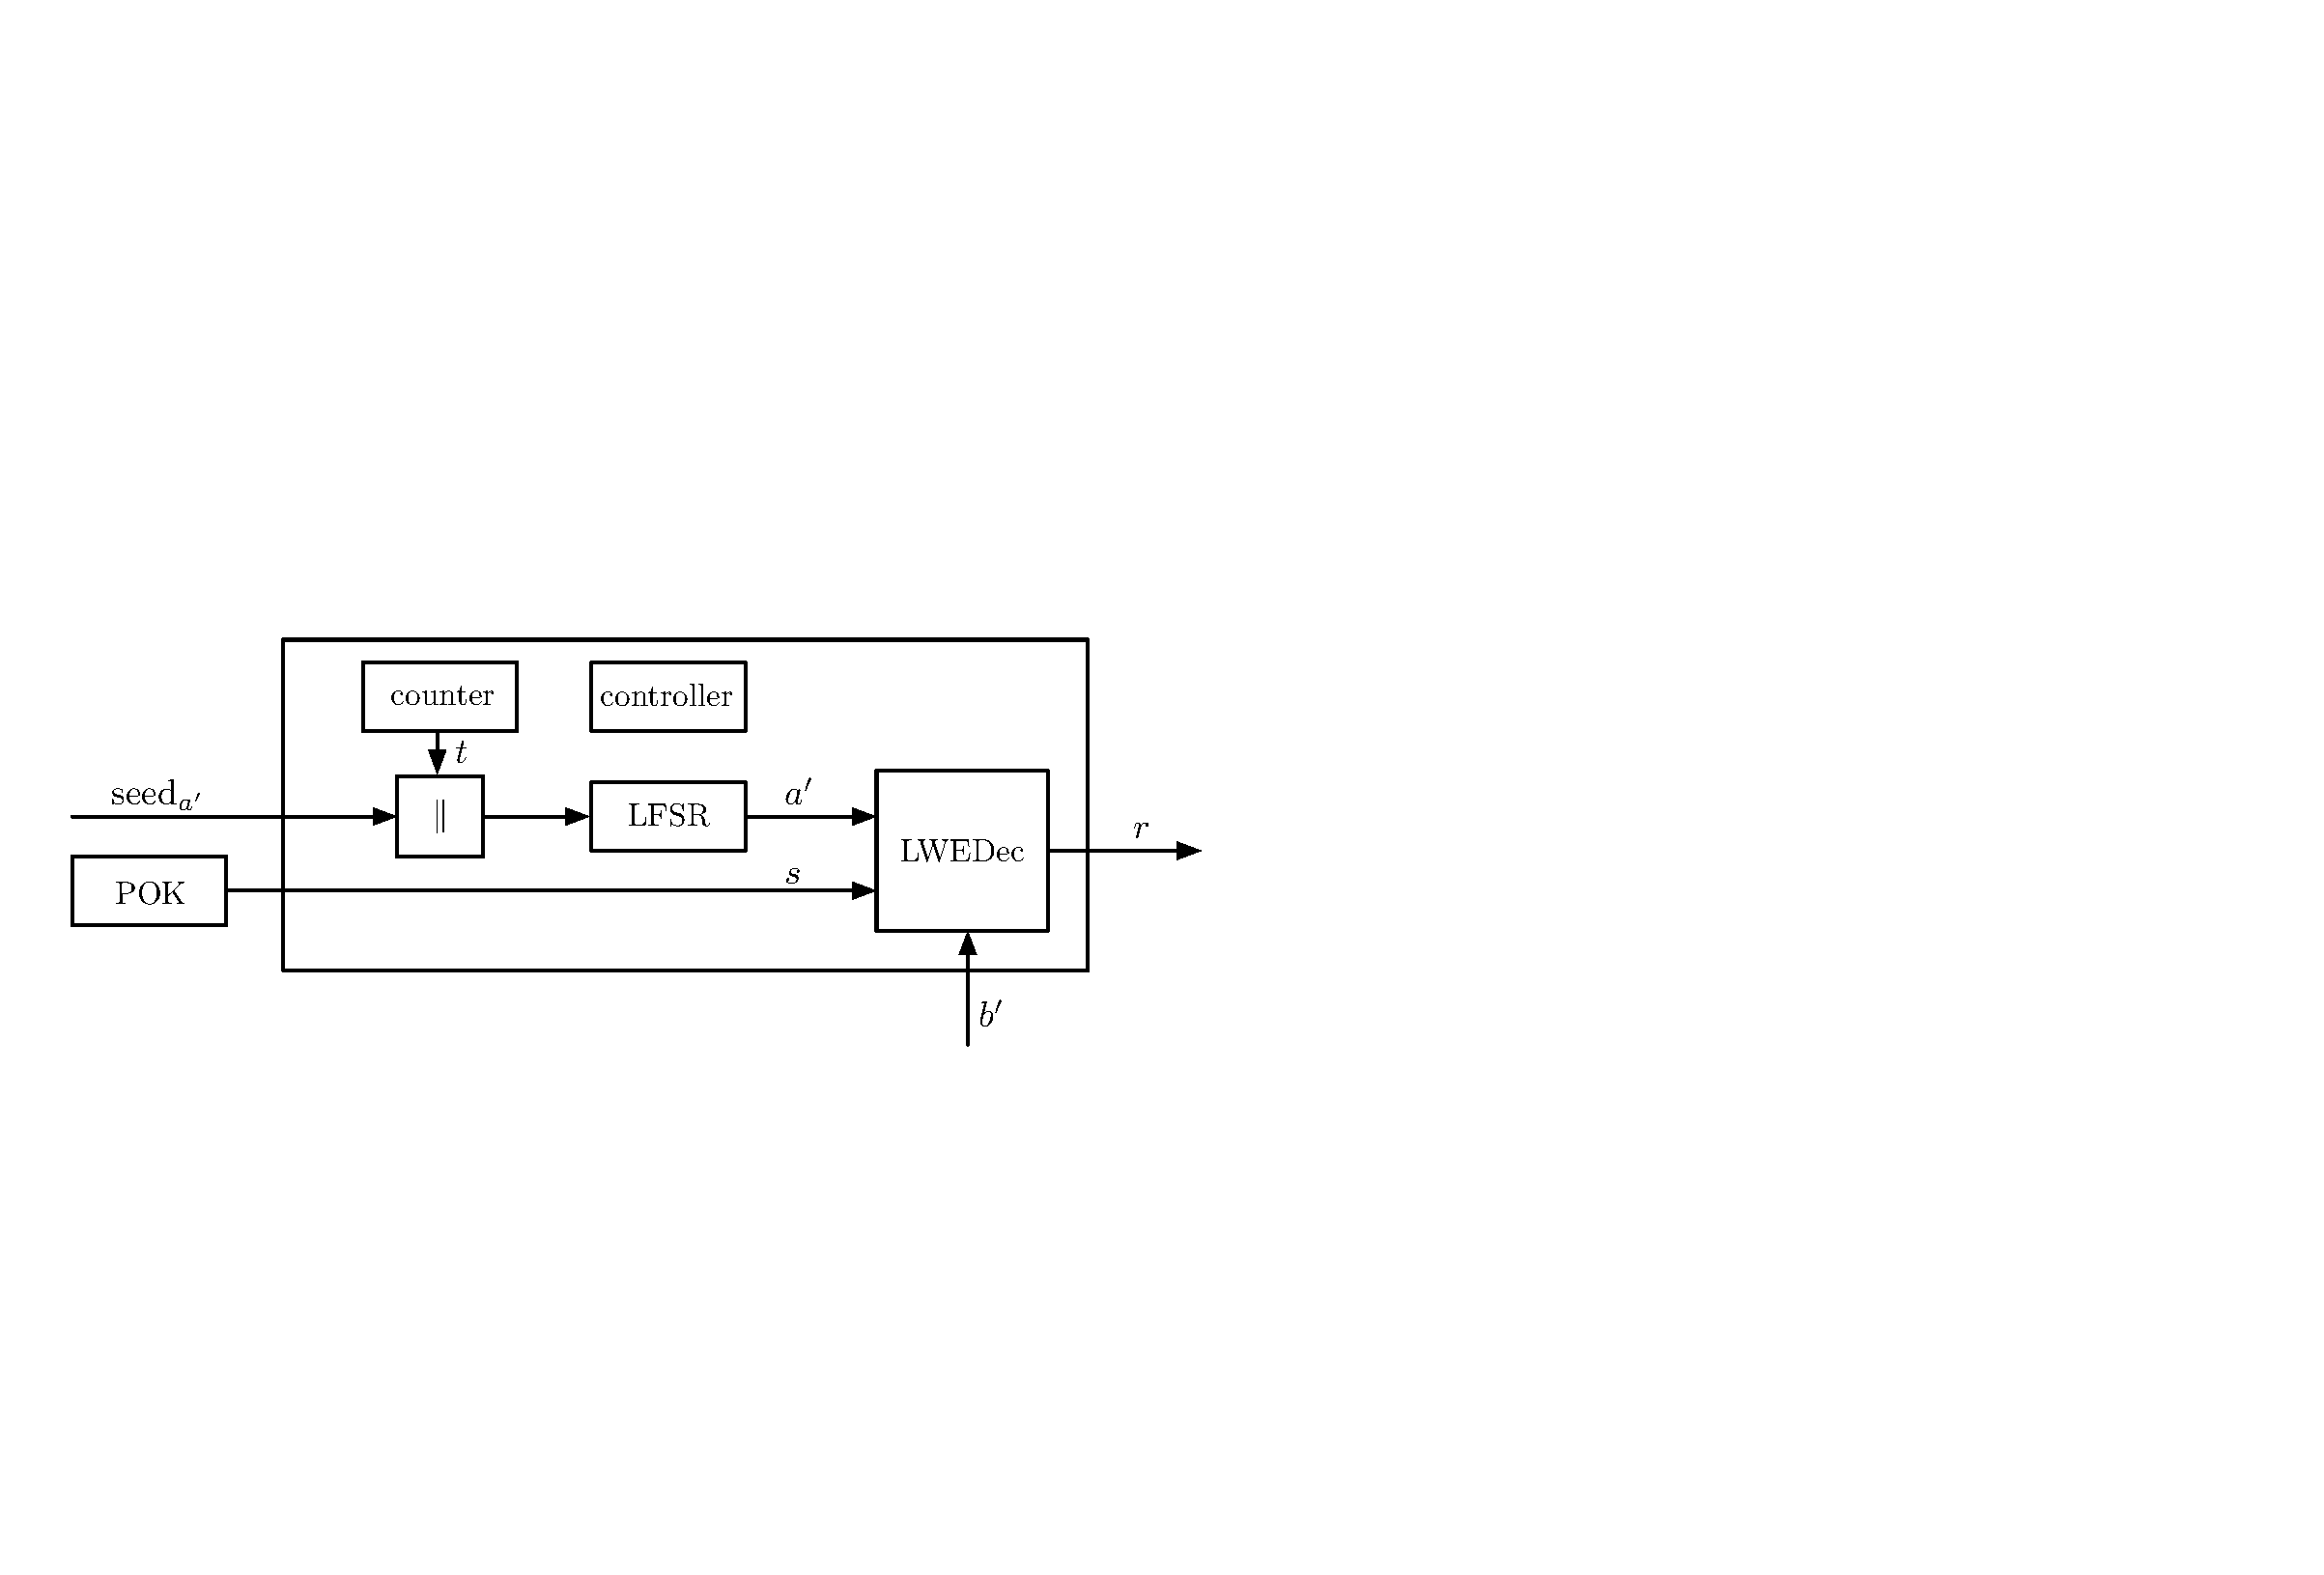
\includegraphics[width = 1.0\linewidth]{./figs/top_level_arch_redraw.pdf}    \caption{Top-level architecture and data flow of the lattice PUF.}
    \label{fig:fpga_impl}
\end{figure}
%\textcolor{red}{The theoretical security guarantees in Section \ref{sec:lwe} shows that an LWE decryption function can be used as a strong PUF with challenges generated from a ciphertext distribution. 
%In this section, we first derive design parameters for the LWE decryption function and show that such a direct implementation of lattice PUF is inefficient in resource constrained environments due to high-ratio of ciphertext to plaintext. 
%As we will illustrate in the following, an LWE decryption function with a 128-bit concrete ML hardness requires transmitting $128.8K$ challenge bits in order to produce a $100$-bit response string. We then solve this problem \emph{by exploiting distributional relaxations allowed by recent work in space-efficient LWEs}. The proposed strategy allows introducing a low-cost PRNG based on an LFSR and transmitting only a small seed, which results in a dramatic reduction of effective challenge size. Next, we introduce a simple defense to protect our PUF against a standard active attack on the LWE decryption function. We then demonstrate two parallelization strategies that reduce response latency. Finally, we introduce a RFE, which is a low-overhead fuzzy extractor, and show its use in an end-to-end authentication scheme.}

The top-level architecture of the proposed lattice PUF is shown in Figure \ref{fig:fpga_impl}.



\subsection{Construct Strong PUF from LWE Decryption Function}
\label{sec:lwe_dec}
\begin{figure}[t!]
    \centering
    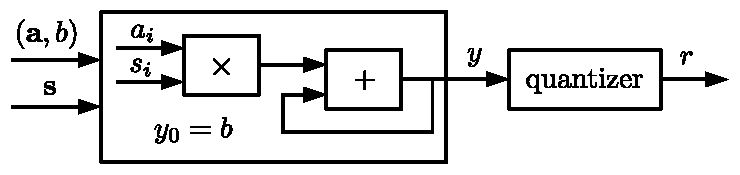
\includegraphics[width = 0.8\linewidth]{./figs/lwe_dec.pdf}
    \caption{Architecture of LWE decryption function.}
    \label{fig:lwedec}
\end{figure}

Figure \ref{fig:lwedec} shows the architecture of LWE decryption function. 
It takes a binary challenge vector $\mathbf{c} = \{c_0,c_1,\ldots,c_{N-1}\}$ of size $N = (n+1)\log q$ which maps to a ciphertext $(\mathbf{a},b)$ in the following way:
\begin{align*}
a_i &= \sum_{j=0}^{\log q-1}c_{(i-1)\log q+j}2^j,\; \forall i\in \{1,2,\ldots,n\}, \\
b &= \sum_{j=0}^{\log q-1}c_{n\log q+j}2^j. 
\end{align*}
Here $a_i$ denotes the $i$-th element of the integer vector $\mathbf{a}\in\mathbb{Z}_q^n$.
In this paper, without specification, $\log(x)$ refers to $\log_2(x)$.
Similarly, the private key $\mathbf{s}$ for the corresponding LWE decryption function is realized by a binary secret key $\mathbf{W} =\{W_0,W_1,\ldots,W_{n\log q-1}\} $ of size $n\log q$:
\begin{equation*}
s_i=\sum_{j=0}^{\log q-1} W_{(i-1)\log q+j} 2^j,\; \forall i\in \{1,2,\ldots,n\}.
\end{equation*}
A modulo-dot-product $b-\innerprod{\mathbf{a},\mathbf{s}}$ is computed using the modulo-multiply-accumulate unit. 
It can be implemented in a serial way using $n$ stages. 
Recall that all additions and multiplications are performed in modulo $q$.
Since $q$ is a power of $2$ in our construction, modulo addition and multiplication can be naturally implemented by integer addition and multiplication that keep only the last $\log q$-bit result. 
Finally the response $r$ is produced by a quantization operation $r = Q(b-\innerprod{\mathbf{a},\mathbf{s}})$: 
\begin{equation*}
Q(x) = \begin{cases}
	0& x \in [0,\frac{q}{4}]\cup(\frac{3q}{4},q-1],\\
	1& x \in (\frac{q}{4},\frac{3q}{4}].
\end{cases}
\end{equation*}

The computation above can be directly implemented as a strong PUF with $2^N$ CRPs since it maps a challenge vector $\mathbf{c}\in \{0,1\}^N$ into a binary response $r\in\{0,1\}$.
We now discuss parameter selection for the LWE decryption function. 
In general, we seek to find design parameters such that 
(1) the resulting PUF has excellent statistical properties, such as uniformity, uniqueness, and reliability, 
(2) successful ML attacks against it require an un-affordably high time complexity in practice, and 
(3) its hardware implementation costs are minimized. 

Prior theoretical arguments establish the impossibility of a polynomial-time attacker. 
To guarantee practical security, we need to estimate the number of samples and the actual running time (or a number of CPU operations) required for a successful ML attack. \cite{regev2009lattices} shows that a small number of samples are enough to solve an LWE problem, but in an exponential time. 
Thus, we refer to runtime as concrete ML resistance (or ML hardness) and say that a PUF has $k$-bit ML resistance if any successful ML attack requires at least $2^k$ operations. 
We adopt the estimator developed by Albrecht \emph{et al.} \cite{albrecht2015concrete} to estimate concrete ML hardness. 
The concrete hardness of an LWE problem increases with the increase of LWE parameters $n$, $q$, and $\alpha$ for all types of attacks.
Recall that $n$ represents the lattice dimension, $q$ represents the range of integer for each dimension, and $\alpha$ reflects the noise level in CRP (ciphertext) generation.
For a given set of parameters, the estimator compares the complexity of several most effective attacks, including decoding, basis reduction, and meet-in-the-middle attacks %\cite{chen2011bkz,howgrave2007hybrid,lindner2011better}. 
\cite{howgrave2007hybrid,lindner2011better}. 
We utilize the estimator in a black-box fashion to find the set of parameters with the target of $128$-bit concrete ML resistance. 

We consider two metrics of implementation cost, both of which scale with $n$: the number of challenge and secret bits needed ($n\log q$), and the number of multiply-accumulate (MAC) operations ($n$).
This motivates the need to decrease $n$.
%\begin{figure}[t!]
%\centering
%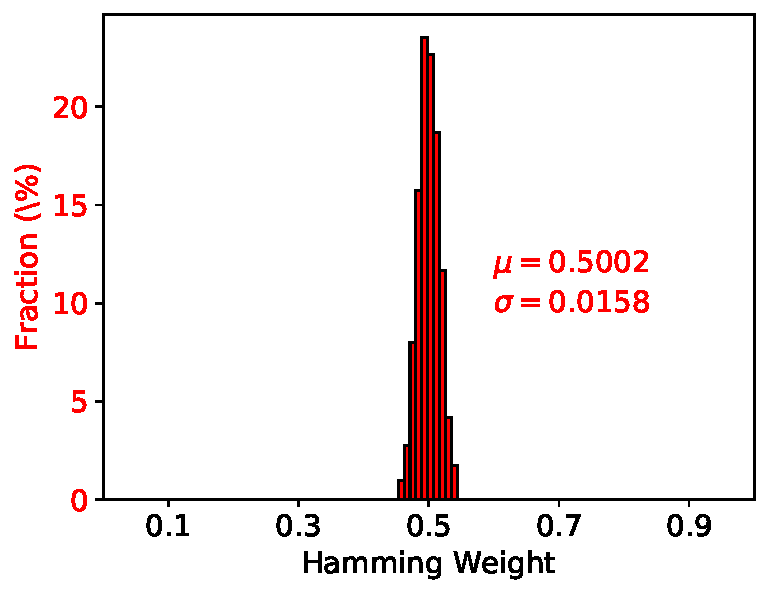
\includegraphics[width = 0.55\linewidth]{./figs/1_bit_HW}
%\caption{CRPs changes radically even with 1 bit POK change.}
%\label{fig:1_bit_hw}
%\end{figure}

%For conventional PUFs, such as APUF and SRAM PUF, an output error is due to environmental noise, e.g. delay changes in APUF and FET strength changes in SRAM PUF with both voltage and temperature.
%In contrast, 
Output errors of the lattice PUF come from two sources: (1) environmental errors of secret bits, and (2) errors of decryption during response generation.
The former can be thought as the failure of key reconstruction in POKs.
Figure \ref{fig:1_bit_hw} shows the hamming-distance between CRPs generated using error-free POKs and POKs with 1 bit error.
Since a single bit-flip completely changes the challenge-response behavior of LWE decryption function, the failure rate of key reconstruction needs to be low, e.g. $10^{-6}$ (as widely adopted in other PUF applications \cite{maes2012pufky}).
Section \ref{sec:result} describes how the target failure rate can be achieved via a conventional FE based on the error-correcting codes.
The latter corresponds to the decryption error and is orthogonal to errors in the secret key $\mathbf{s}$. 
Recall that in CRP generation of the lattice PUF, a bit of plaintext $r$ is sampled and the ciphertext $\mathbf{c}$ is produced by a noisy encryption function $\mathbf{c}=\Enc(r)$. 
Given ciphertext $\mathbf{c}$ as input challenge, the decryption function can output a wrong response $r^\prime\neq r$ when the accumulated error $\sum_{i\in S} e_i$ in the encryption function exceeds the decision boundary.

%\begin{figure}[t!]
%\centering
%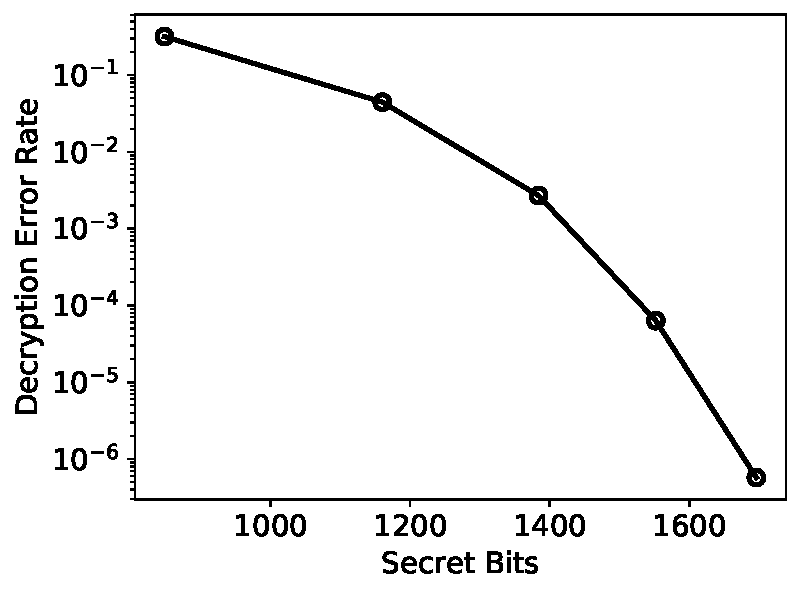
\includegraphics[width = 0.55\linewidth]{./figs/dec_error_secret_bits}
%\caption{Super-exponential decrease of decryption error rate with the increase of secret bits.
%The analysis is done for 128-bit concrete hardness.}
%\vspace{-1.0em}
%\label{fig:num_POK_vs_dec_err}
%\end{figure}

\begin{figure}[t!] 
    \centering
  \subfloat[\label{fig:1_bit_hw}]{%
       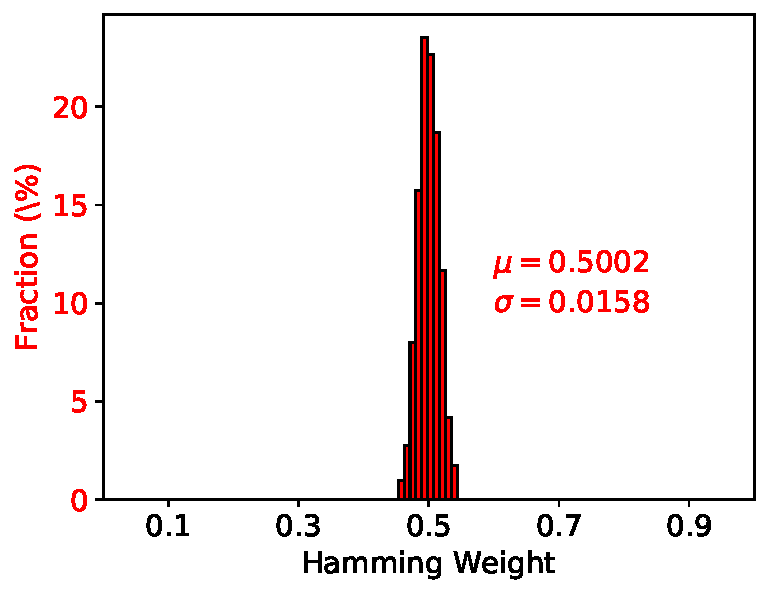
\includegraphics[width=0.48\linewidth]{./figs/1_bit_HW}}
    \hfill
  \subfloat[\label{fig:num_POK_vs_dec_err}]{%
        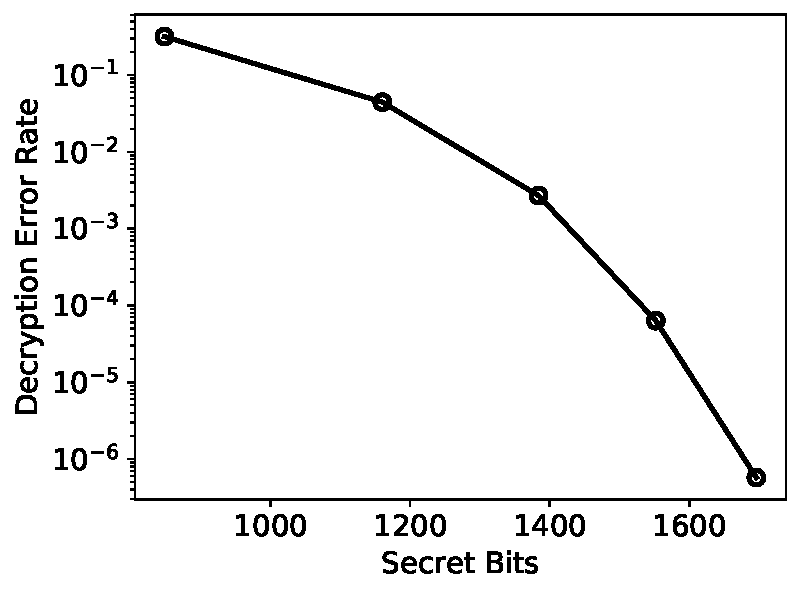
\includegraphics[width=0.5\linewidth]{./figs/dec_error_secret_bits}}
  \caption{(a) CRPs change radically even with 1 bit POK change. (b) Super-exponential decrease of decryption error rate with the increase of secret bits. The analysis is done for 128-bit concrete hardness.}
  \label{fig: lattice_puf_features} 
\end{figure}

%The model for evaluating the decryption error rate is shown in Section \ref{sec:bg}.
In order for a strong PUF to be used in direct authentication, its decryption error rate should be small enough for reliable distinguishability of long strings.
We set the target around $2\%$.
Figure \ref{fig:num_POK_vs_dec_err} explores the trade-off between the number of secret bits and the decryption error rate needed for $128$-bit concrete ML hardness.
It shows that, at fixed concrete ML hardness, the decryption error rate decreases super exponentially with the number of secret bits. 

Considering the design metrics above, a feasible set of parameters is found using the estimator in \cite{albrecht2015concrete}.
By setting $n=160$, $q=256$, $m=256$ and $\alpha = 2.20\%$, we achieve a lattice PUF with $128$-bit concrete hardness and a decryption error rate of $1.26\%$.

In order to get a $1$-bit response, $(n+1)\log q = 1288$ bits need to be sent to the lattice PUF as a challenge.
For direct authentication applications, usually around $100$ bits of responses are required. Therefore, the direct implementation described so far would require $C = 128.8K$ challenge bits.
This high ratio of challenge length to response length limits its practical use in many scenarios when communication is expensive.

%\textcolor{red}{A class of attacks which manipulates public helper data to exploit PUF generated keys can compromise PUF security \cite{helper_data_manipulation}. Such attacks apply to pairing-based PUFs (for instance, RO PUFs), and require public access to helper data. However, such attacks may not be applicable to our construction, since our POK is based on the SRAM PUF, which follows a completely different mechanism. In addition, the possibility of the attacks can be reduced by limiting public access to helper data. Therefore, the helper data manipulation attack is not a major concern for our design.}


\vspace{-0.5em}
\subsection{Challenge Compression through Distributional Relaxation}
\label{sec:lfsr}
%We now describe the proposed strategy based on space-efficient LWE that overcomes the limitation on communication inefficiency.
The LWE decryption function described in Section \ref{sec:lwe_dec} requires a challenge $\mathbf{c}$ in the form $\mathbf{c}=(\mathbf{a},b)$ to be sent from the server to the PUF. 
To represent vector $\mathbf{a} \in \mathbb{Z}_q^n$ requires $n\log q$ bits while to represent scalar $b \in \mathbb{Z}_q$  requires only $\log q$ bits. 
Thus, the major cost of transmission lies in sending $\mathbf{a}$. 
We wish to avoid sending $\mathbf{a}$ directly and, instead, to send a compressed (shorter) version of $\mathbf{a}$  and re-generate its full-size version on the PUF.
Our approach is enabled by the recent results on the distributional behavior of $\mathbf{a}=\mathbf{A}^T\mathbf{x}$ \cite{akavia2009simultaneous} and the concept of space-efficient LWE \cite{galbraith2013space}.

Recall that $b$ is given by: 
\begin{align*}
    b&=\mathbf{b}^T\mathbf{x}+r\floor{q/2}\\
    &= (\mathbf{A}\mathbf{s}+\mathbf{e})^T\mathbf{x}+r\floor{q/2}\\
    &=(\mathbf{A}^T\mathbf{x})^T\mathbf{s}+\mathbf{e}^T\mathbf{x}+r\floor{q/2}.
\end{align*}
First, we replace the component $\mathbf{a}=\mathbf{A}^T\mathbf{x}$ by $\mathbf{a}^*$ uniformly randomly sampled from $\mathbf{Z}_q^n$. That allows us to represent challenge $\mathbf{c} = (\mathbf{a},b)$:
\begin{equation*}
    \begin{cases}
    \mathbf{a}= \mathbf{A}^T\mathbf{x}\\
    b = (\mathbf{A}^T\mathbf{x})^T\mathbf{s}+\mathbf{e}^T\mathbf{x}+r\floor{q/2}
    \end{cases}
\end{equation*}
as $\mathbf{c}^*=(\mathbf{a}^*,b^*)$:
\begin{equation*}
    \begin{cases}
    \mathbf{a}^*\\
    b^*=\mathbf{a}^{*T}\mathbf{s}+\mathbf{e}^T\mathbf{x}+r\floor{q/2}
    \end{cases}.
\end{equation*}
In \cite{akavia2009simultaneous}, it is proven that distribution of $\mathbf{c}^*=(\mathbf{a}^*,b^*)$ is statistically close to the original ciphertext distribution, therefore the required security properties are preserved.  

The advantage of the above approximation is that, as shown by \cite{galbraith2013space}, several low-complexity  PRNGs are capable of producing an output string $\mathbf{a}^\prime$ suitably close to $\mathbf{a^*}\in\mathbb{Z}^n_q$ within the context of LWE cryptosystem. In particular, an LFSR is an especially simple PRNG having the right properties.
Specifically, a vector $\mathbf{a}^\prime$ generated by an LFSR provides similar concrete security guarantees against standard attacks on LWE, such as CVP reduction, decoding, and basis reduction \cite{galbraith2013space}.
This is because LFSR-generated $\mathbf{a}^\prime$ maintains good properties including:
\begin{itemize}
    \item it is hard to find ``nice'' bases for a lattice with basis from LFSR-generated $\mathbf{a}^\prime$;
    \item given an arbitrary vector in $\mathbb{Z}_q^n$, it is hard to represent it as a binary linear combination of LFSR-generated $\mathbf{a}^\prime$'s;
    \item it is hard to find a short vector $\mathbf{w}$ that is orthogonal to LFSR-generated $\mathbf{a}^\prime$'s.
\end{itemize}

The ability to rely on a simple PRNG to produce $\mathbf{a}^\prime$ allows a dramatic reduction in challenge transfer cost. 
Now, the challenge $\mathbf{c}^\prime$ contains only a small $\text{seed}_{\mathbf{a}^\prime}$ into the PRNG and the corresponding $b^\prime$ as
\begin{align*}
    b^\prime&=(\mathbf{a}^\prime)^T\mathbf{s}+\mathbf{e}^T\mathbf{x}+r\floor{q/2}\\
    &= \LFSR{(\text{seed}_{\mathbf{a}^\prime})}^T\mathbf{s}+\mathbf{e}^T\mathbf{x}+r\floor{q/2}.
\end{align*}
Here $\LFSR(\cdot)$ denotes the output generated by an LFSR.


%\begin{figure*}[t!]
%\centering
%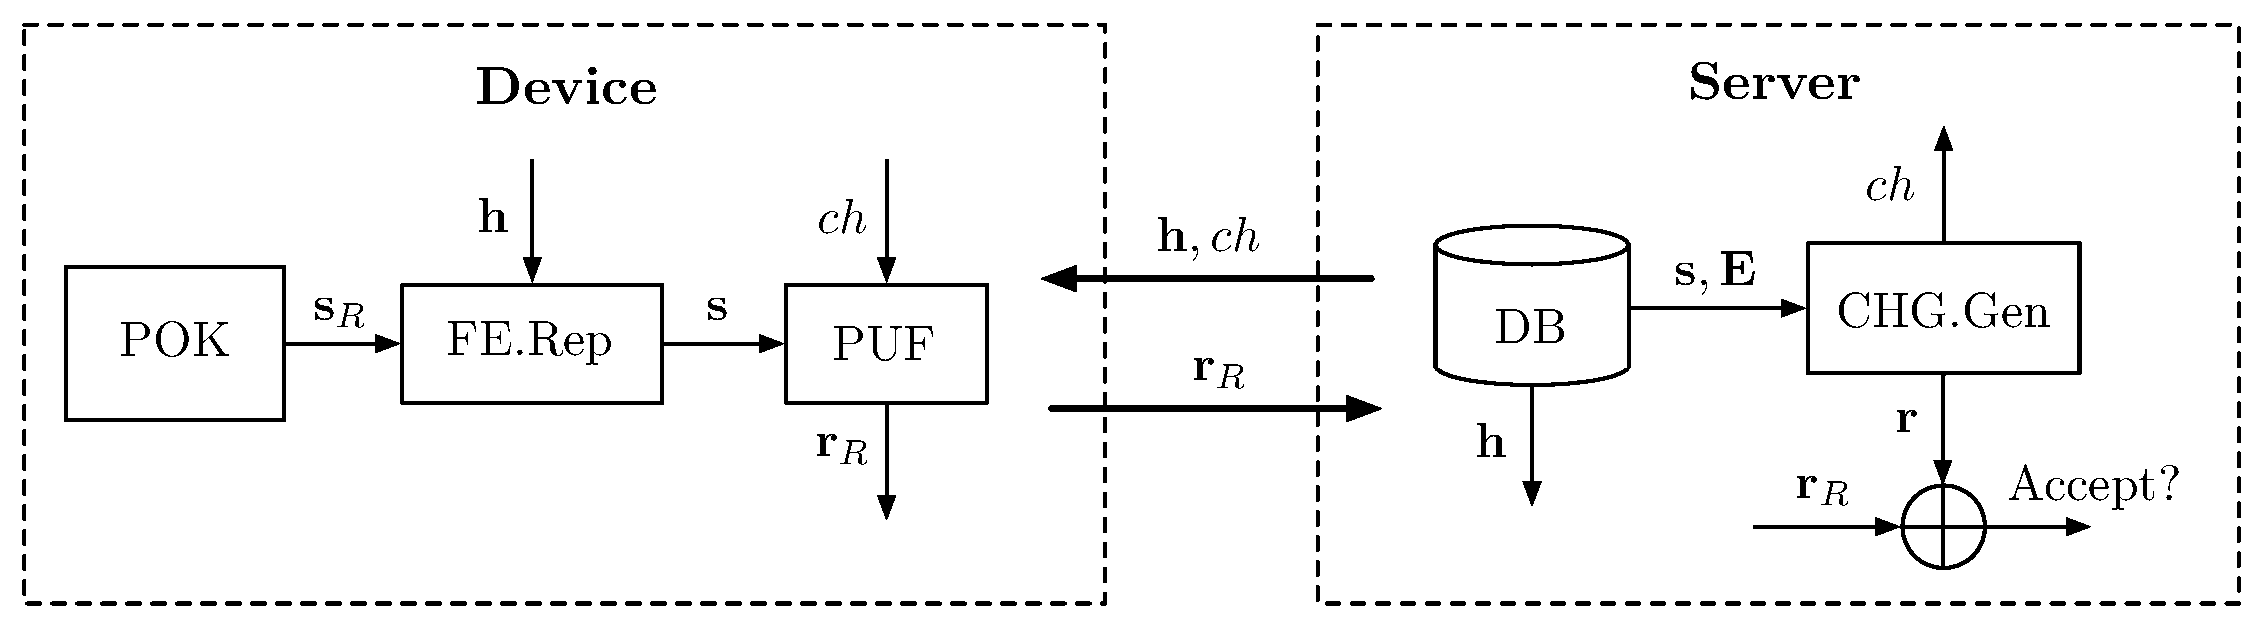
\includegraphics[width = 0.85\linewidth]{./figs/authen_system}
%\caption{Building blocks of the authentication scheme with the lattice PUF.}
%\label{fig:authen_system}
%\end{figure*}

%\begin{figure}[t!]
%\centering
%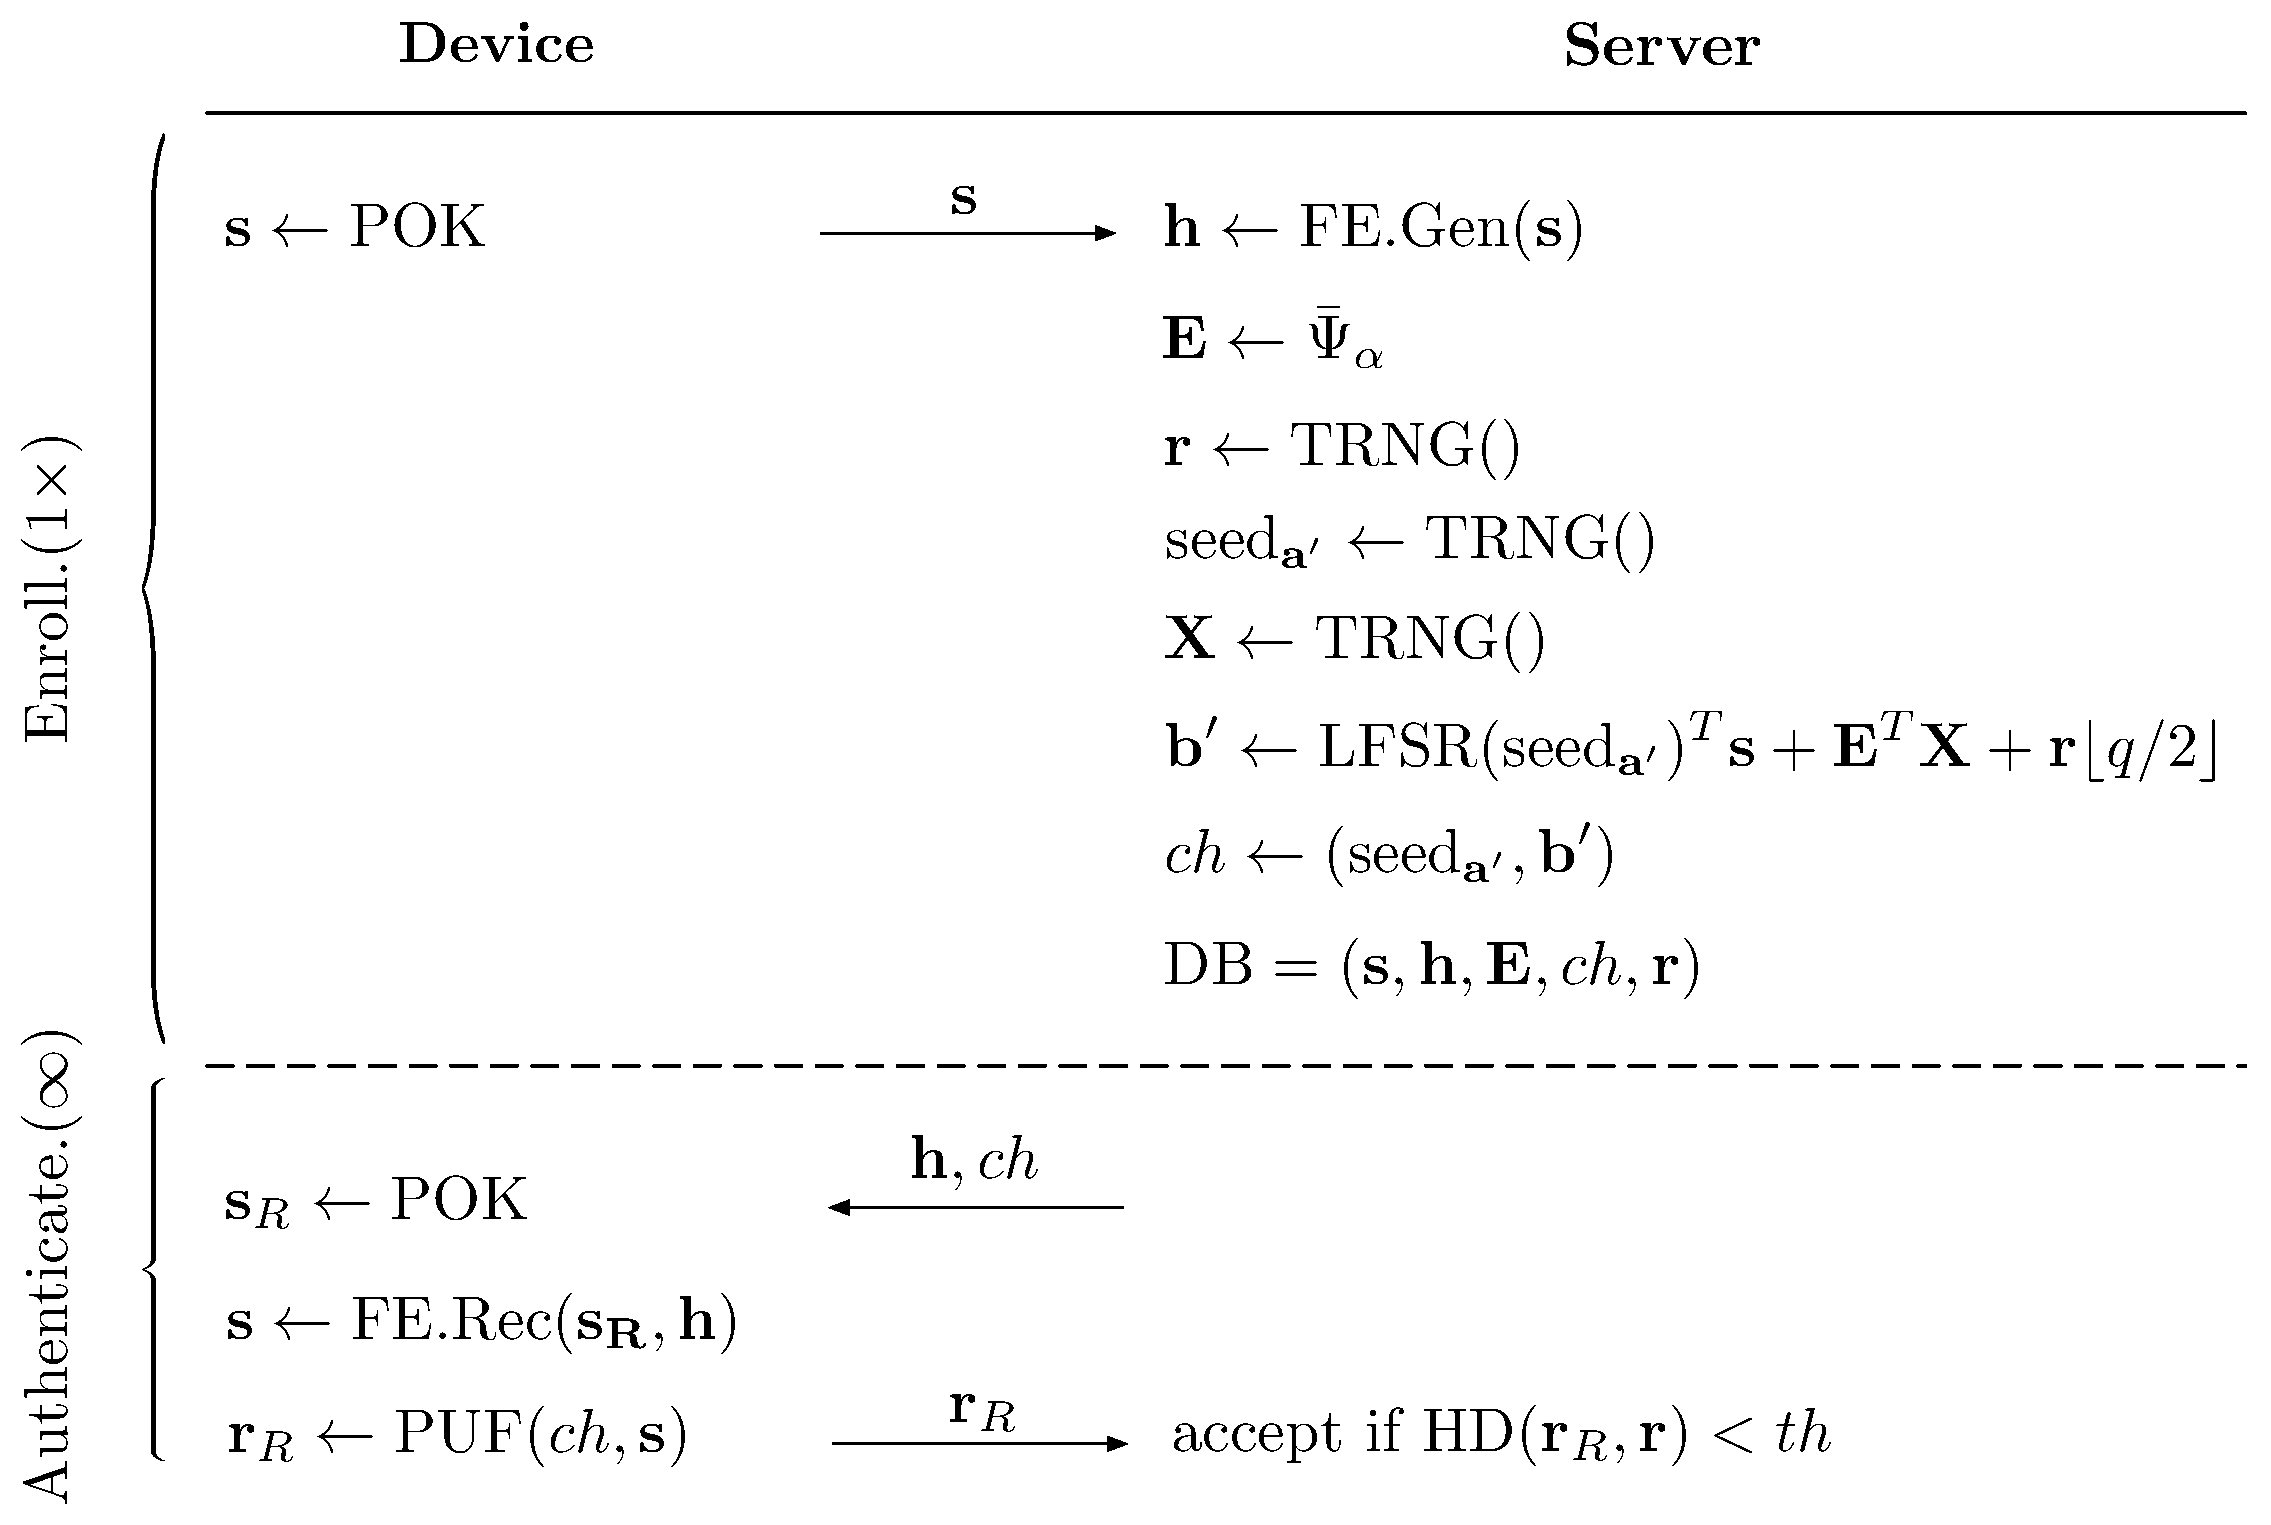
\includegraphics[width = 1.0\linewidth]{./figs/protocol}
%\caption{End-to-end authentication system with the lattice PUF.}
%\label{fig:protocol}
%\end{figure}

With LWE parameters chosen as Section \ref{sec:lwe_dec}, using a seed of length $l=256$ is able to reduce the challenge length from $1288$ to $256+8=264$ per one bit of response. 
The improvement of efficiency becomes more pronounced for generating multiple responses:
This is because $\mathbf{a}^\prime_1 \ldots \mathbf{a}^\prime_t$ can be generated sequentially from the $l$-bit seed, so that only the seed and $b^\prime_1,\ldots, b^\prime_t \in Z_q$ are required to be sent to the PUF side. 
$100$ bits of responses now require only transmitting $256+100\times\log 256 = 1056$ bits for challenges.

\subsection{Countermeasure for Active Attack}
\label{sec:counter}
%The focus of the paper is a PUF secure against passive attacks in which the observed challenges can be used to derive an internal model of the PUF. 
%However, the LWE decryption function is vulnerable to an active attack that supplies arbitrary input challenges. 
%(As we show, this risk also carries into an LFSR-based variant). 

We now demonstrate an active attack that compromises security of lattice PUF. The attack is premised on the ability to supply arbitrary challenges (ciphertexts) as inputs to the decryption function. 
The attack proceeds as follows. 
The attacker fixes $\mathbf{a}$ and enumerates all possible $b\in \mathbb{Z}_q$ for challenge $\mathbf{c} = (\mathbf{a},b)$.
As $b$ increases from $0$ to $q-1$, the response $r = Q(b-\innerprod{\mathbf{a},\mathbf{s}})$ changes from  $Q(b-\innerprod{\mathbf{a},\mathbf{s}}) = 0$ to $Q(b+1-\innerprod{\mathbf{a},\mathbf{s}}) = 1$ exactly when $b$ satisfies
\begin{equation*}
b-\innerprod{\mathbf{a},\mathbf{s}} = q/4.
\end{equation*}
We denote this specific value of $b$ as $\hat{b}$. 
The exact value of $\innerprod{\mathbf{a},\mathbf{s}}$ can then be extracted by $\innerprod{\mathbf{a},\mathbf{s}} = \hat{b} - q/4$. 
By repeating this procedure $n$ times, the attacker is able to set up $n$ linear equations (without errors):  
\begin{align*}
\label{eq:secret_eqs}
    \innerprod{\mathbf{a}_0,\mathbf{s}} &= \hat{b}_0 - q/4, \\
    \innerprod{\mathbf{a}_1,\mathbf{s}} &= \hat{b}_1 - q/4, \\
    & \cdots \\
    \innerprod{\mathbf{a}_{n-1},\mathbf{s}} &= \hat{b}_{n-1} - q/4.
\end{align*}
Gaussian elimination can then be used to solve for $\mathbf{s}$, entailing compromising the system. 
%The reason the attack succeeds is that attackers are able to fix $\mathbf{a}$ and use it for multiple values of $b$. 

%We overcome the risk of such an attack by adopting the technique in \cite{yu2016lockdown}: we introduce a self-incrementing counter to embed the counter value into a challenge seed.
To defend against the attack, we introduce a self-incrementing counter to embed the counter value into a challenge seed \cite{yu2016lockdown}.
This makes the attack impossible as the counter restricts the attacker's ability to completely control input challenges to the LWE decryption function.
As a result, the attacker cannot enumerate all values of $b$ while keeping $\mathbf{a}$ unchanged. 
As shown in Figure \ref{fig:fpga_impl}, the concatenation of the challenger-provided seed and the counter value $t$ (i.e. $\text{seed}_{\mathbf{a}'}||t$) is used as the seed for generating $\mathbf{a}$. 
The counter value is public and is incremented by $1$ on each response generation.

\subsection{Latency Optimization via Design Parallelization}
\label{sec: lpuf_par}


%\begin{figure}[t!]
%\centering
%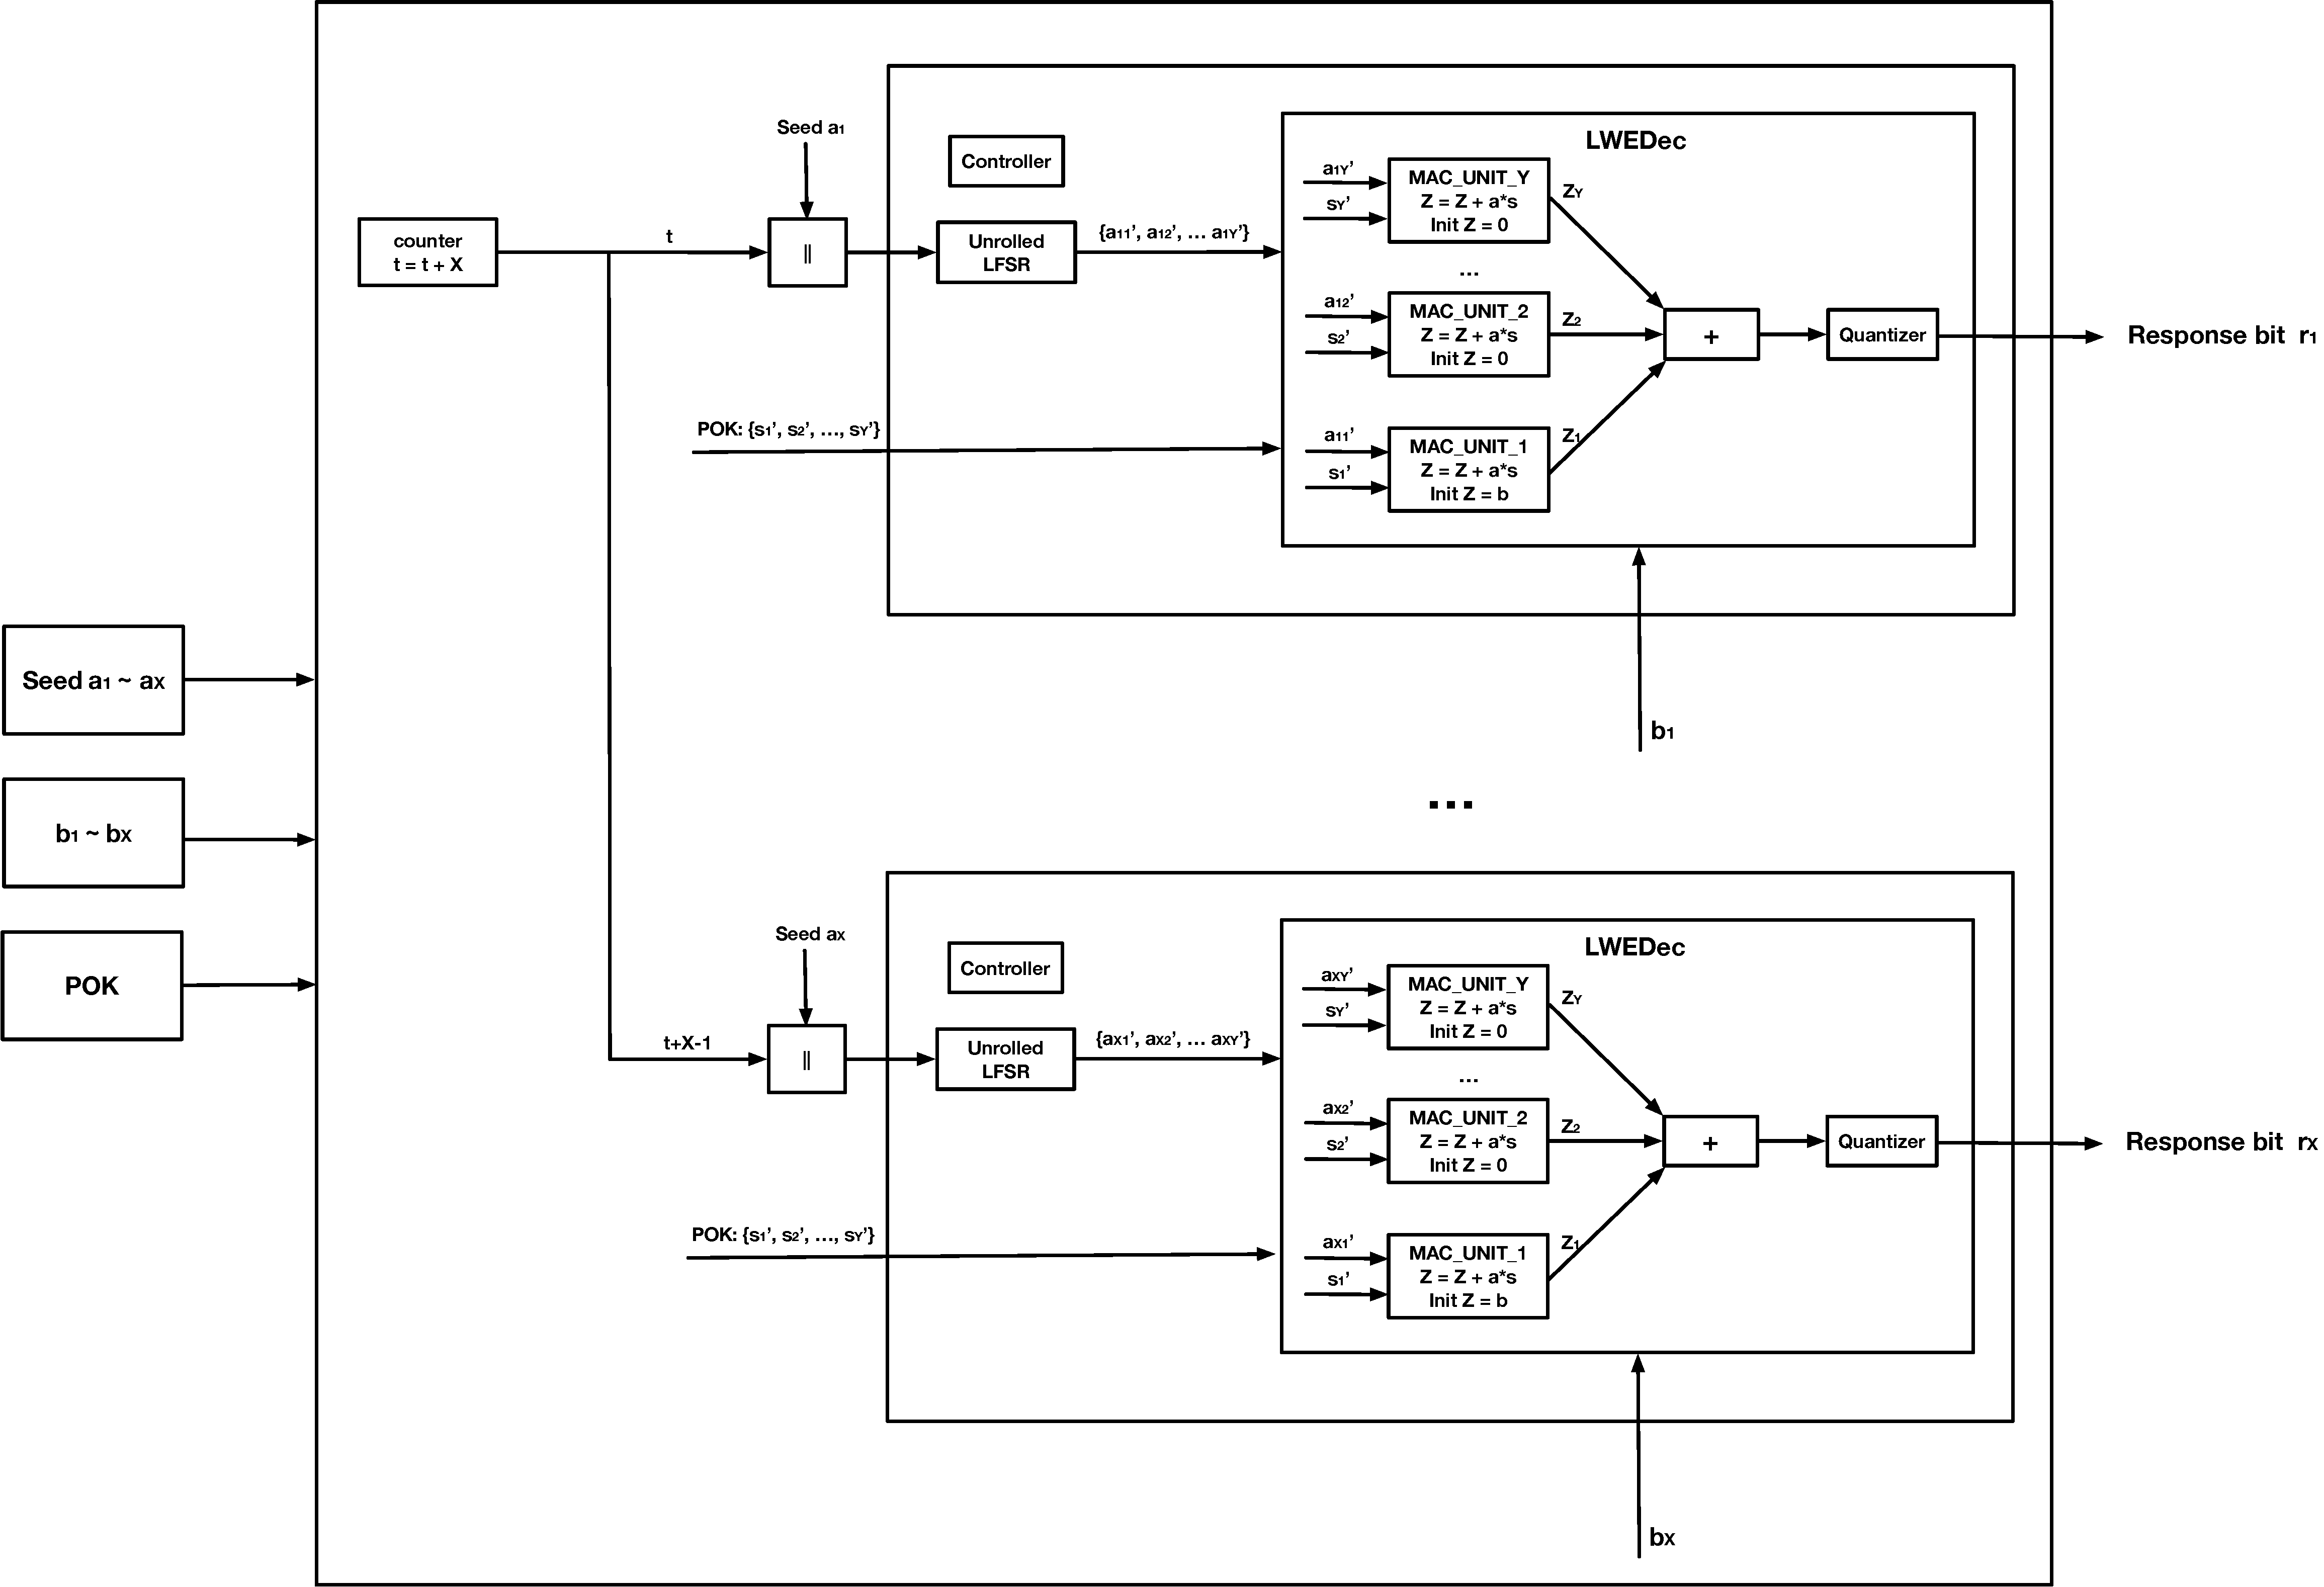
\includegraphics[width = 1.0\linewidth]{./figs/lpuf_p1_p2}
%\caption{Lattice PUF parallelization 3.}
%\label{fig:lpuf_p1_p2}
%\end{figure}

The lattice PUF architecture shown in Fig. \ref{fig:fpga_impl} achieves low hardware implementation cost via a bit-serial design. %The design adopts a single multiply-and-accumulate (MAC) unit and generates a single response bit after multiple sequential MAC operations. 
However, the highly serialized design leads to inefficient utilization of clock cycles resulting in large response latency. To generate one bit of response, the design needs $160$ sequential MAC operations and each MAC needs to wait $8$ cycles until one byte of ciphertext is generated by the bit-serial LFSR. This is undesirable in performance-critical applications. %While the lightweight property is generally desired in a resource constrained environment, latency of response generation is also critical in a PUF-based application. 


We observe that latency is limited by two factors: (1) the LFSR and LWE decryption function (LFSR-LWEDec) datapath produces response bits serially, and (2) the LWE decryption function performs a single MAC sequentially.  We optimize each aspect. %to reduce the overall latency.
%\textcolor{red}{We keep LFSR in the latency-optimized design due to its capability of reducing challenge transmission cost, as illustrated in Section \ref{sec:lfsr}.}

\begin{figure}[t!]
\centering
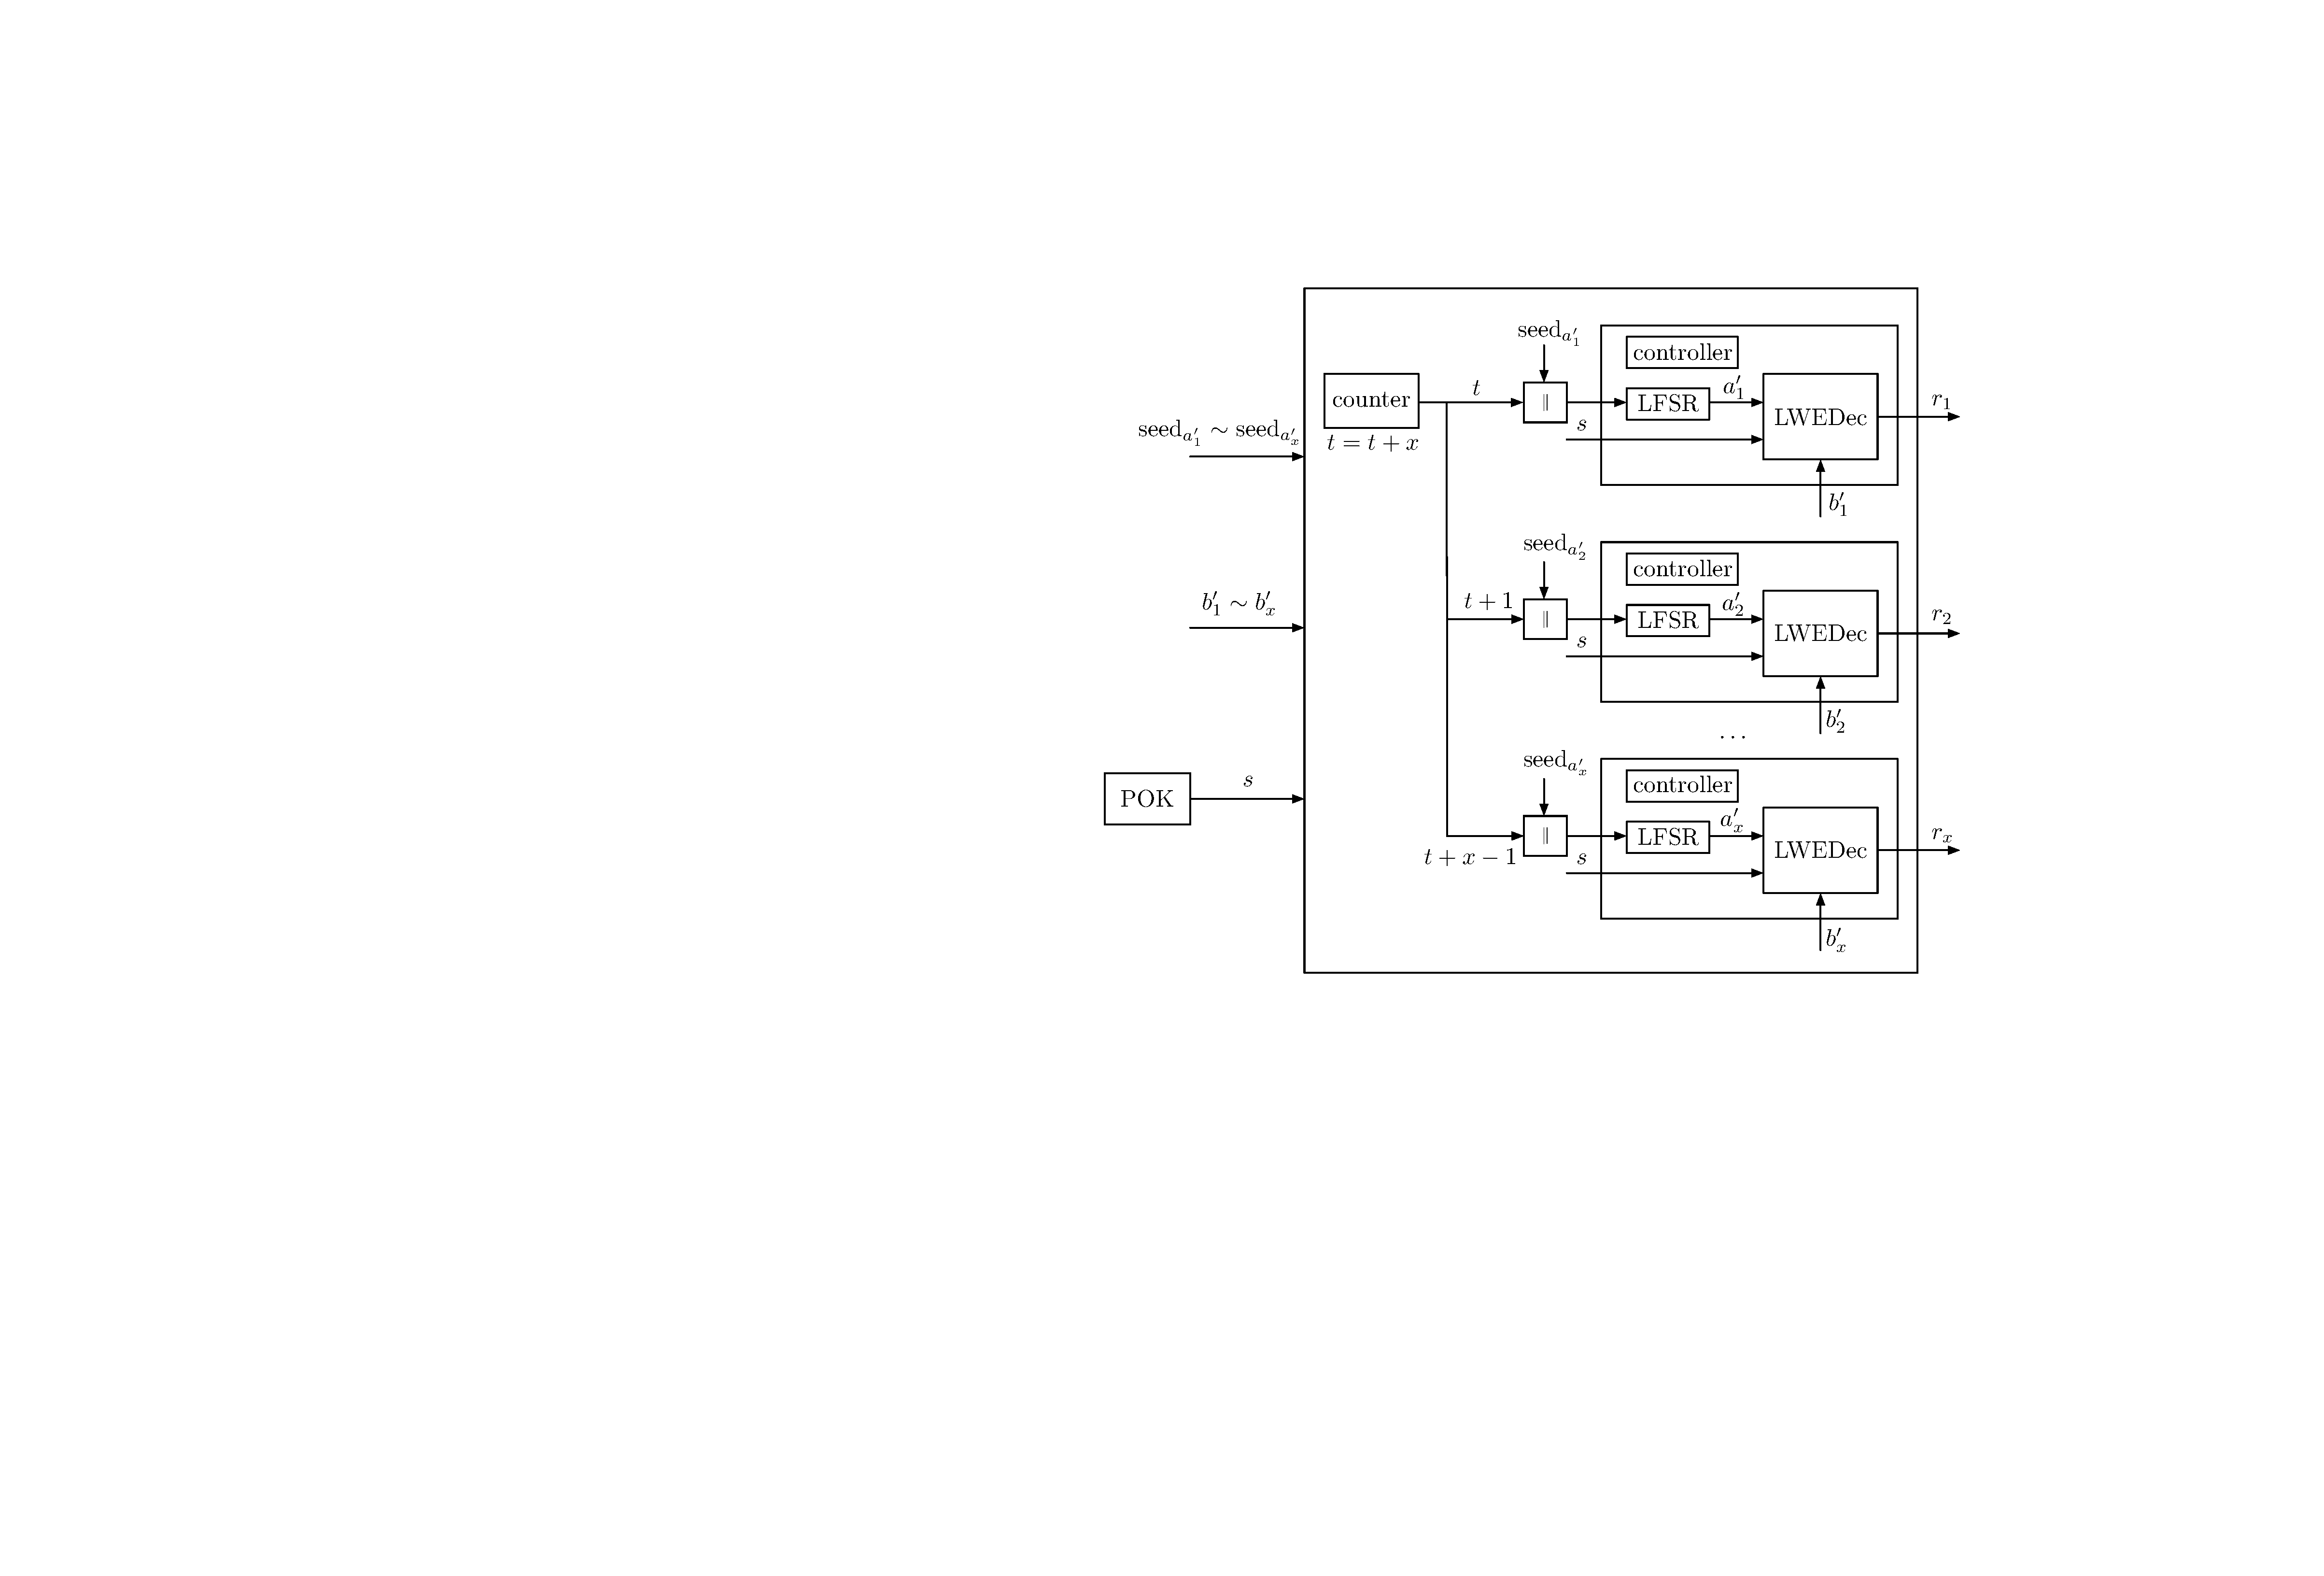
\includegraphics[width = 0.8\linewidth]{./figs/lpuf_p1}
\caption{Reducing latency via a parallel LFSR-LWEDec datapath.}
\label{fig:lpuf_p1}
\end{figure}

We first parallelize the LFSR-LWEDec data-path which implements the functionality in response generation: the LFSR generates ciphertext and LWE decryption function performs modulo MAC operation. Parallelizing it allows multiple response bits to be generated simultaneously, Fig. \ref{fig:lpuf_p1}. Each LFSR-LWEDec data-path uses the same POK, but receives different LFSR seeds and ciphertext inputs. 

We adapt the counter technique described in Section \ref{sec:counter}. %Specifically, we embed an increasing value into the LFSR seed for each LFSR-LWEDec data-path. The increasing values are counted from the output of a main counter, which increments by the number of parallel data-paths for each response generation. 
We embed an increasing counter value into the seed of each datapath, Fig. \ref{fig:lpuf_p1}. %On a design with $P_1$ parallel LFSR-LWEDec data-paths, 
The strategy directly enables $P_1$ times reduction in response generation latency, at the cost of $P_1$ times increase in seed transmission and datapath hardware utilization.

We now investigate how to increase the dot-product throughput in LWE decryption. Since the LWE decryption function contains only a single MAC unit, we increase the number of MACs. However, the throughput of the LFSR limits the overall throughput of the data-path: it produces only a single output bit per cycle. %For each MAC operation, the MAC unit has to wait until a full ciphertext byte ($q=256$) is generated. 
Therefore, to fully utilize the parallel MAC units, the LFSR needs to produce a sufficient number of ciphertext bytes on each cycle. We adopt an unrolled LFSR to increase its throughput.

\begin{figure}[t!]
\centering
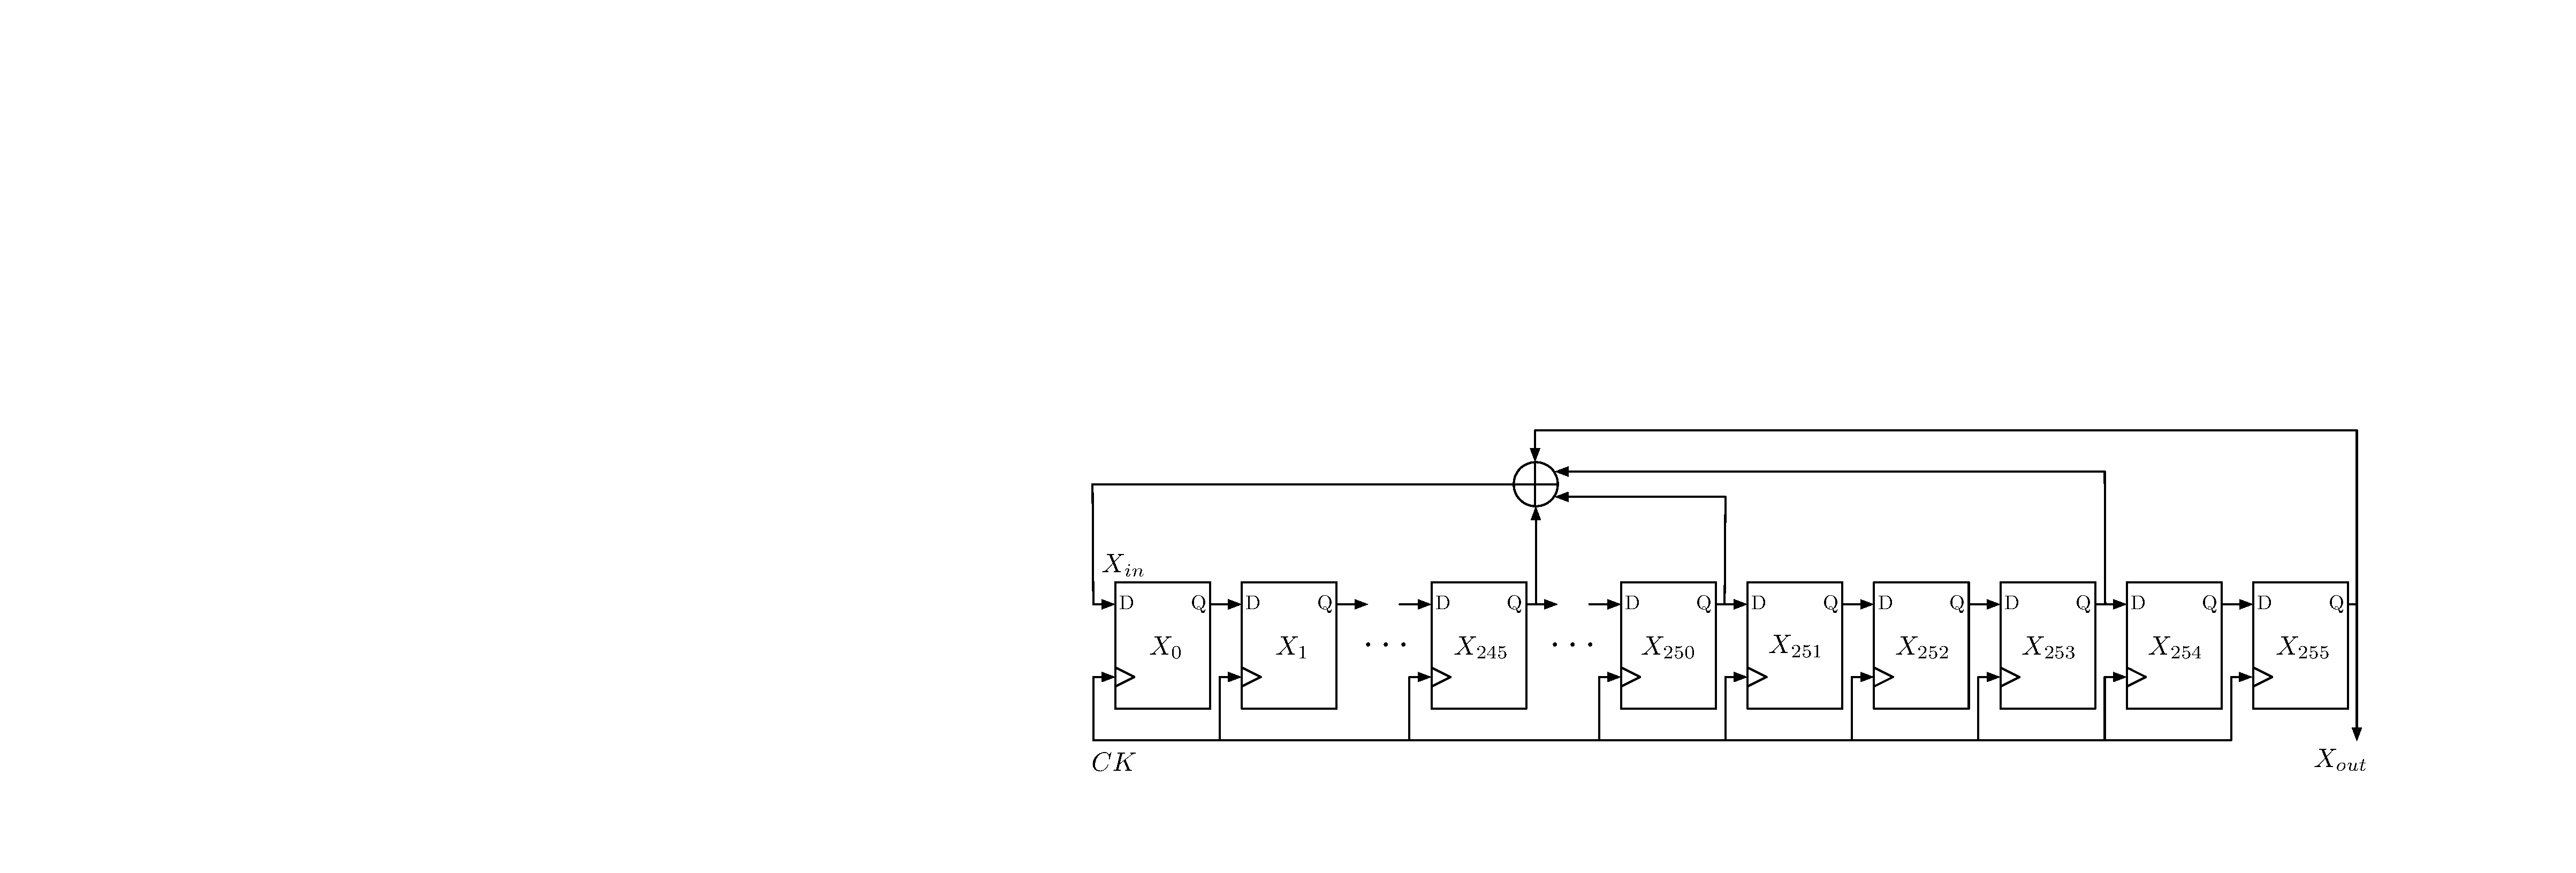
\includegraphics[width = 1.0\linewidth]{./figs/lfsr_baseline_compressed}
\caption{A 256-bit bit-serial LFSR.}
\label{fig:lfsr_baseline}
\end{figure}

\begin{figure}[t!]
\centering
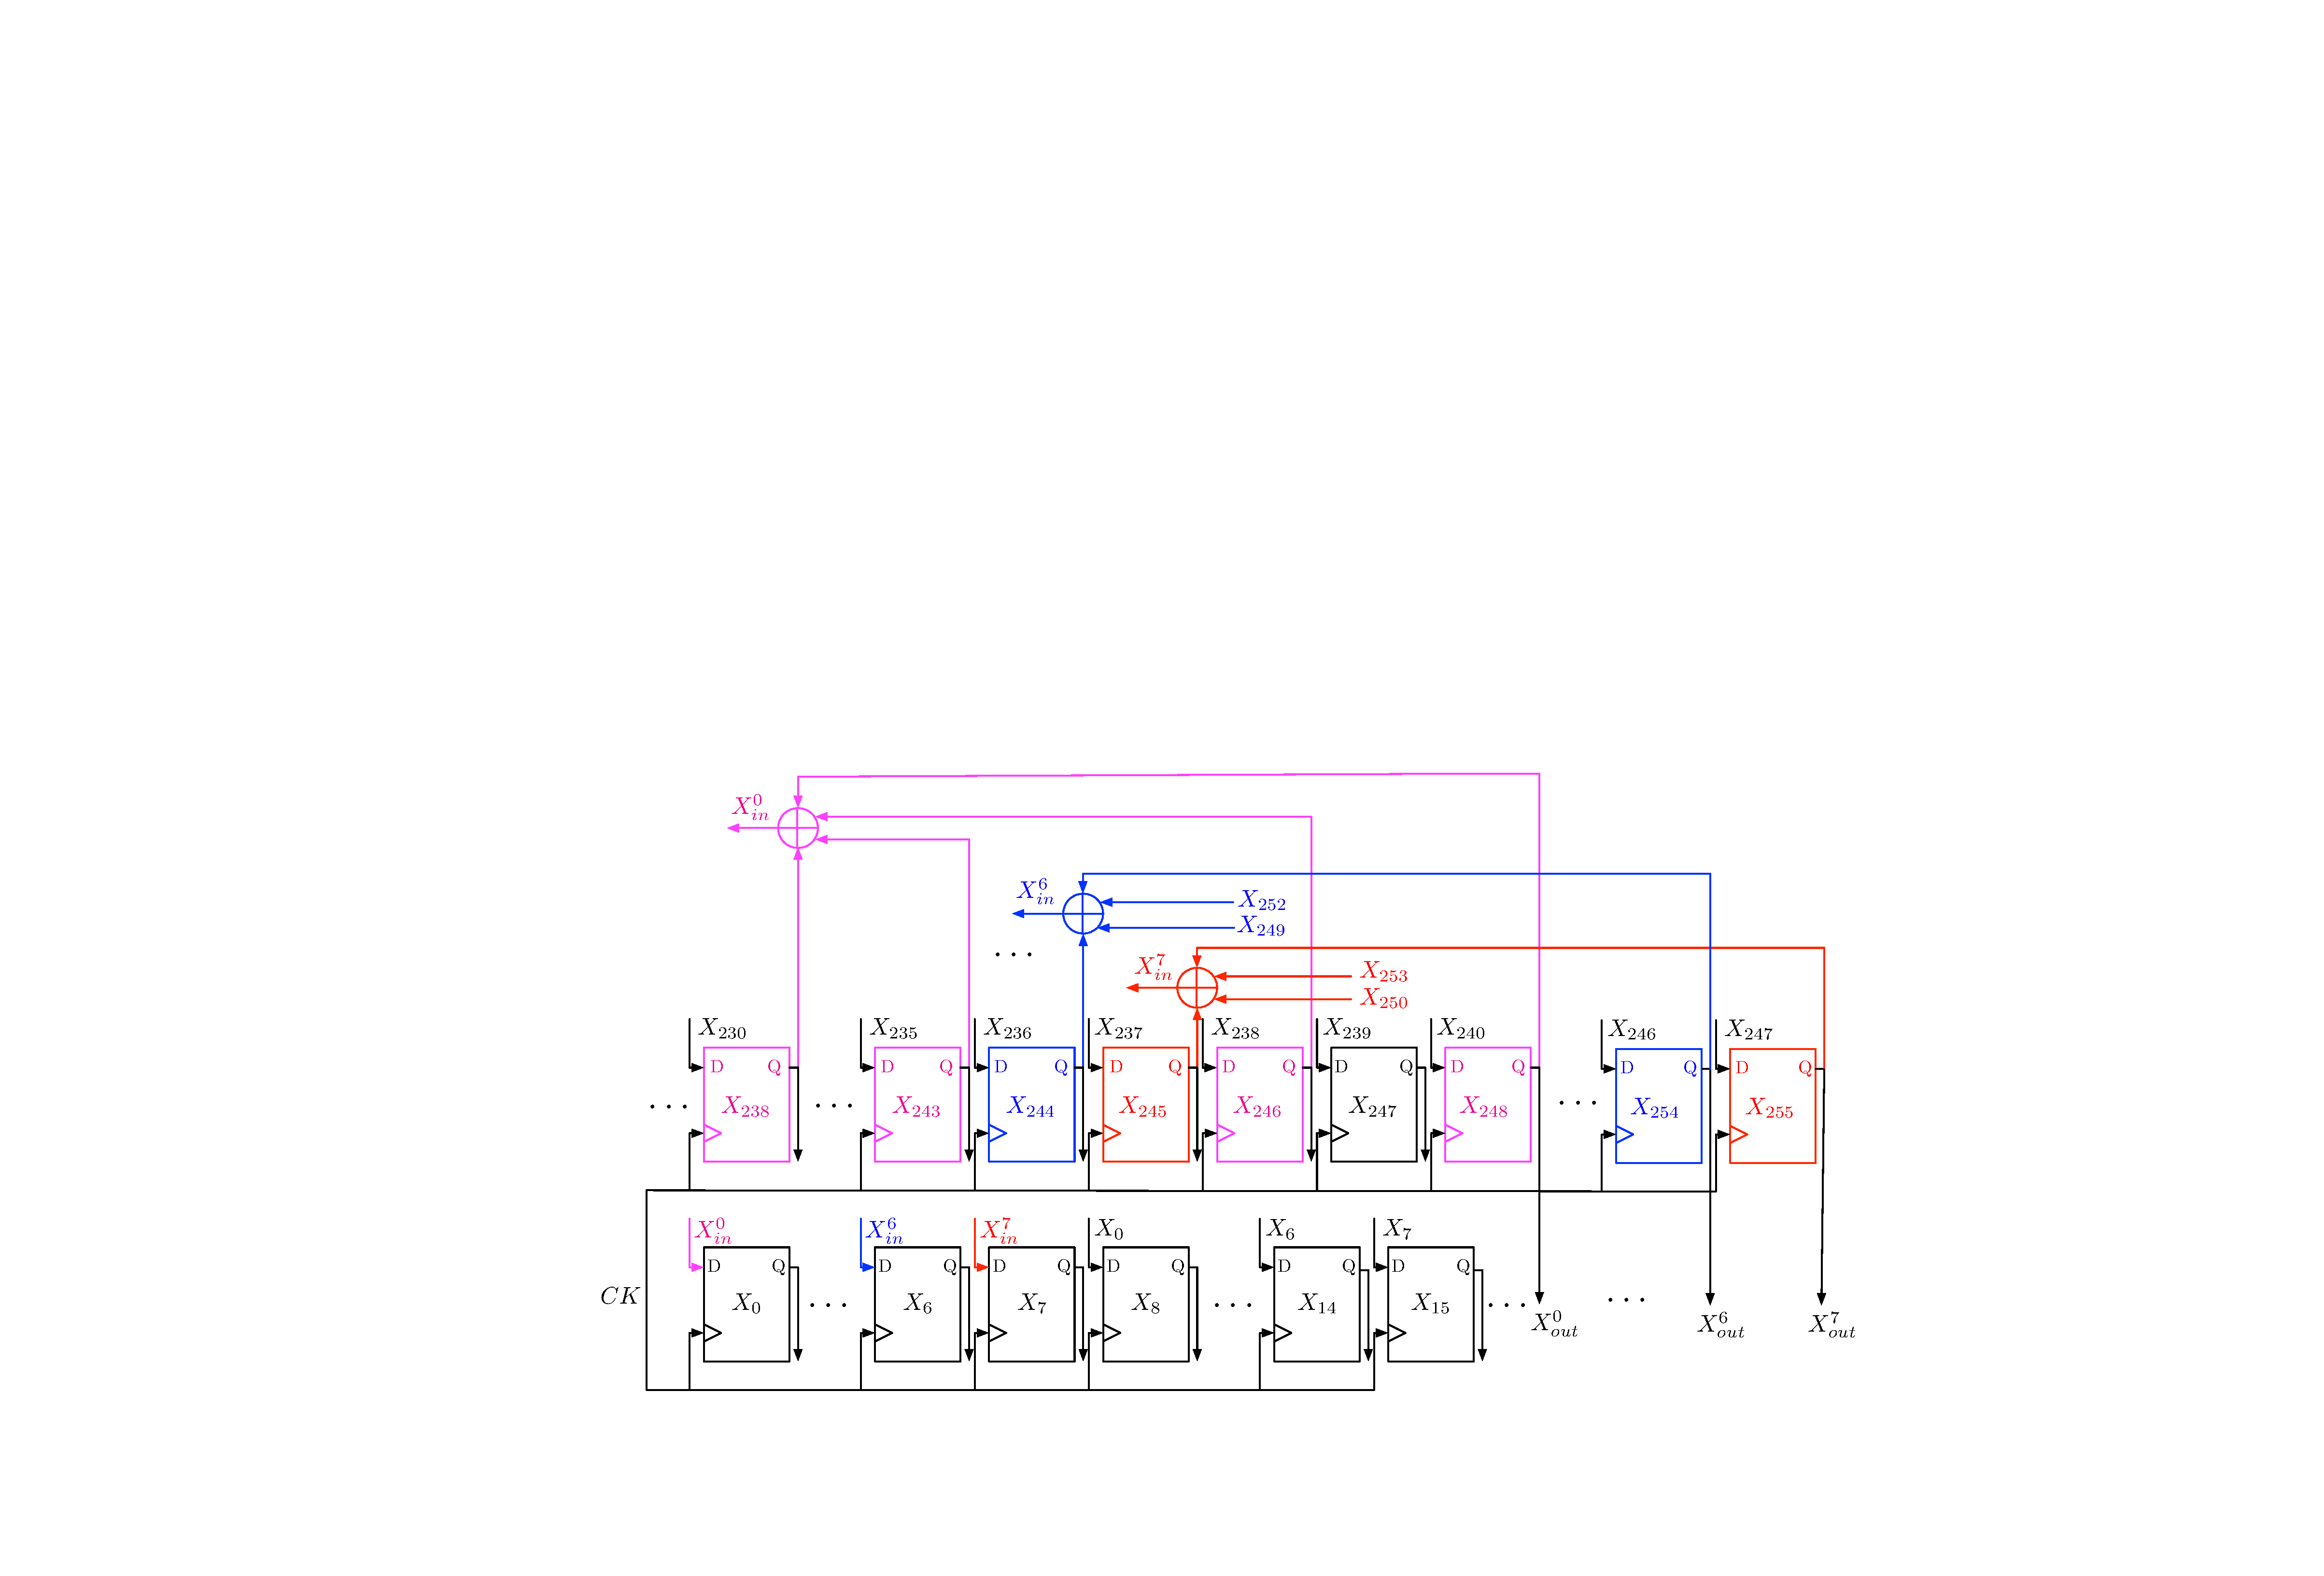
\includegraphics[width = 1.0\linewidth]{./figs/lfsr_unrolled_compressed}
\caption{A 256-bit LFSR unrolled by a factor of 8.}
\label{fig:lfsr_unrolled}
\end{figure}

\begin{figure}[t!]
\centering
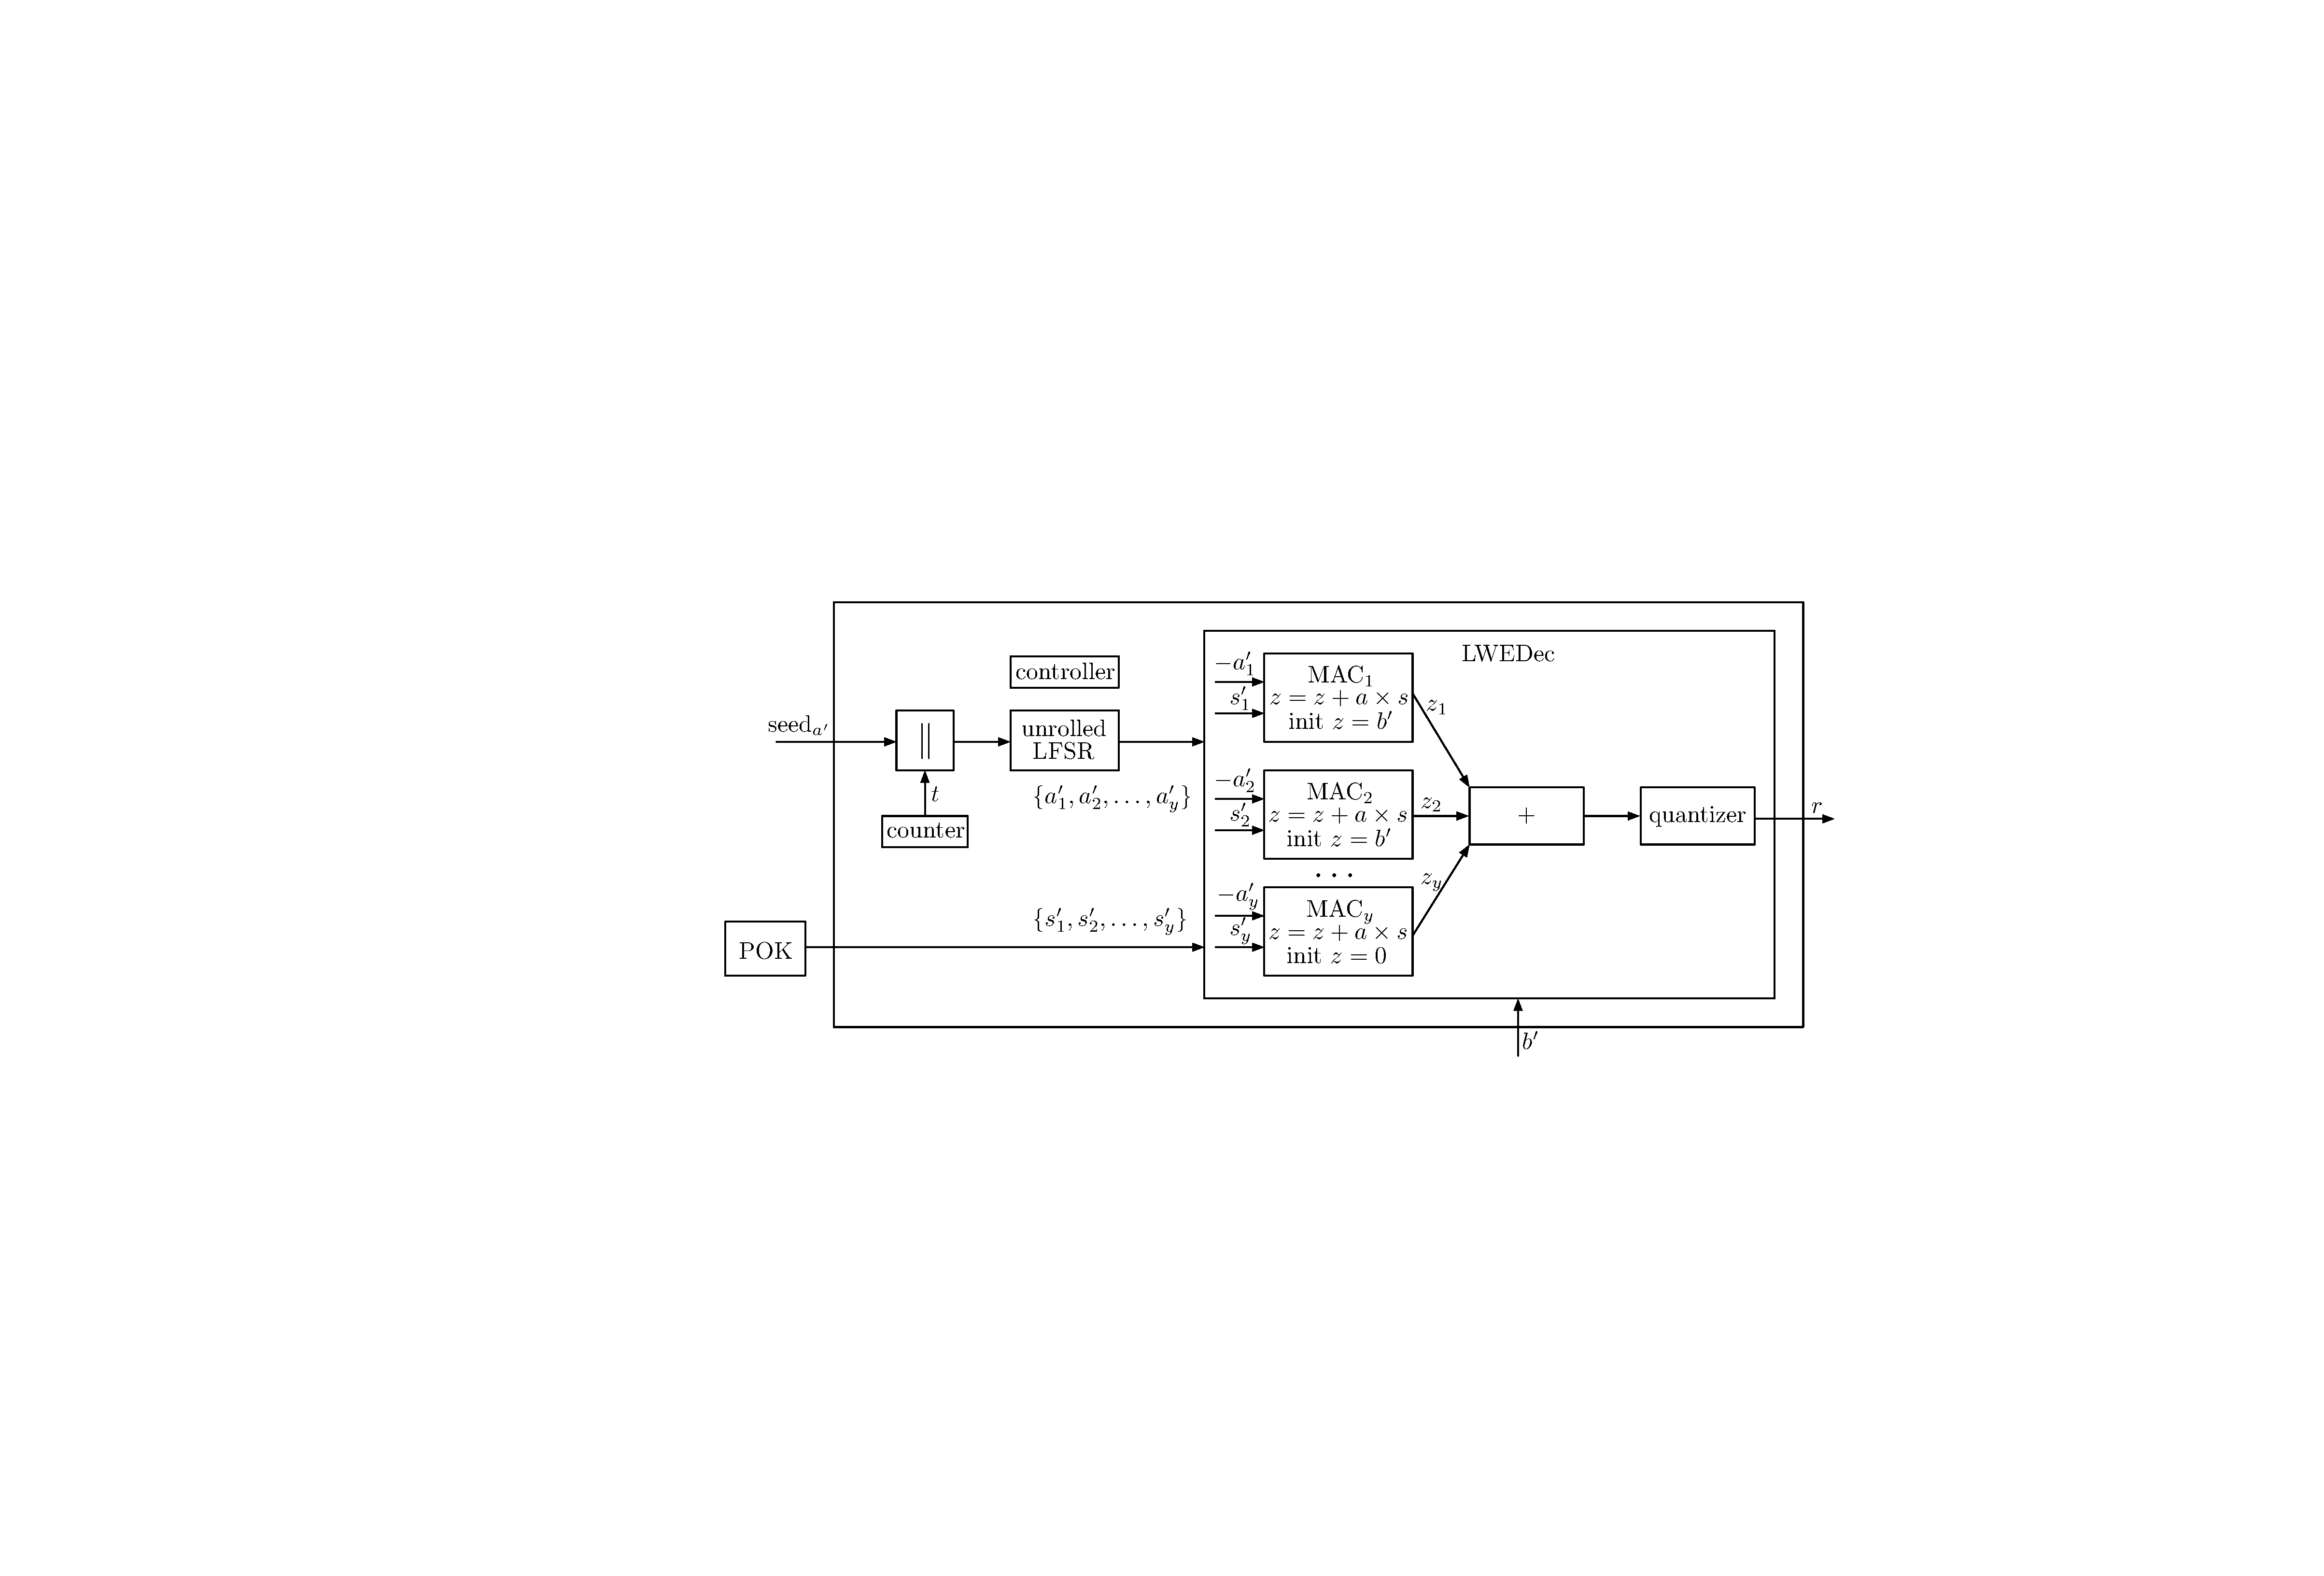
\includegraphics[width = 1.0\linewidth]{./figs/lpuf_p2_large}
\caption{Reducing latency via parallel MAC units.}
\label{fig:lpuf_p2}
\end{figure}

\begin{figure}[t!]
\centering
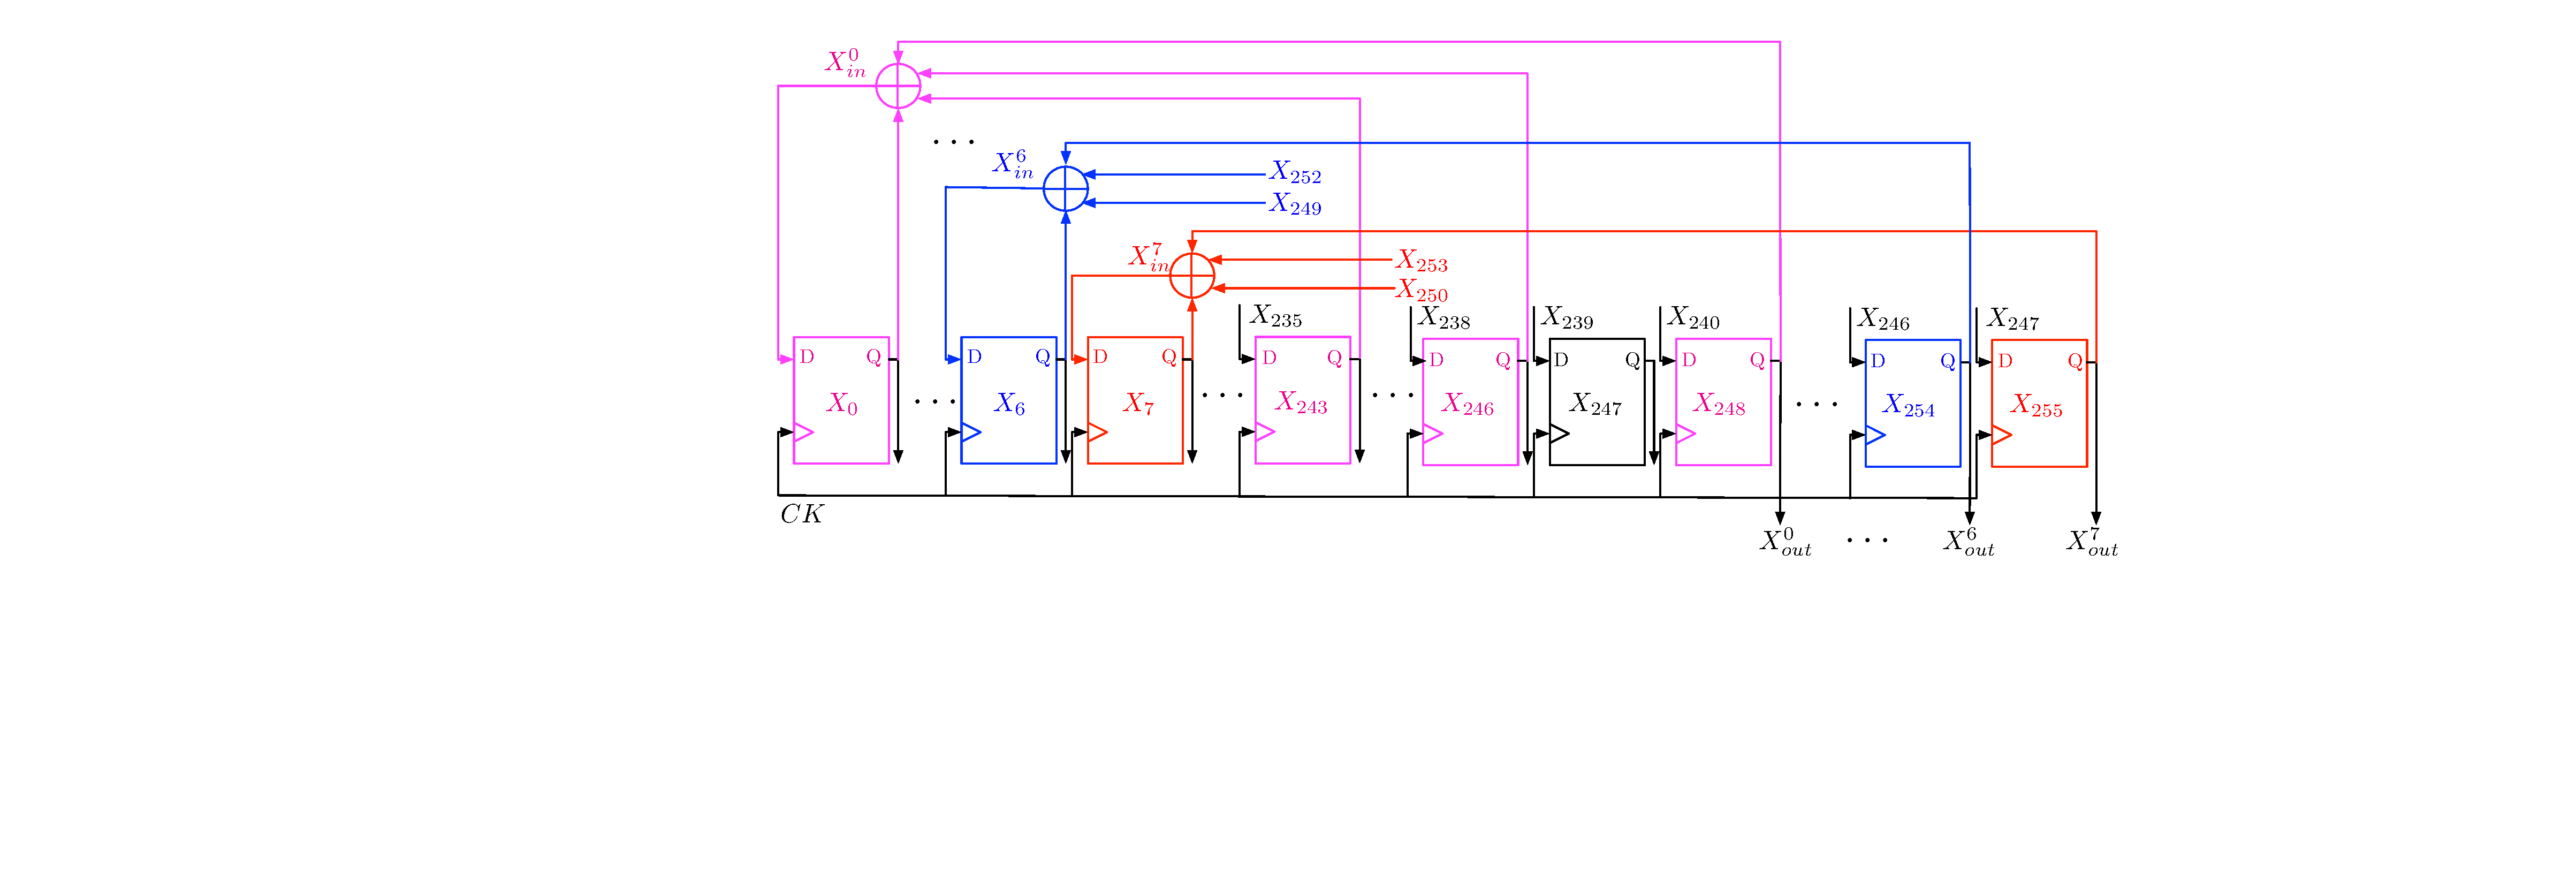
\includegraphics[width = 1.0\linewidth]{./figs/lfsr_unroll_limit_compressed}
\caption{The LFSR generator polynomial limits the maximum unrolling factor. It cannot produce feedback bits for more than $8$ consecutive cycles due to the constraint of $X_{7}$.}
\label{fig:lfsr_unrol_limit}
\end{figure}

An unrolled LFSR is functionally equivalent to the bit-serial LFSR, capable of producing multiple bits per cycle %\cite{cycle_efficient_lfsr, unrolled_lfsr_ref_2, unrolled_lfsr_ref_3}. 
\cite{cycle_efficient_lfsr, unrolled_lfsr_ref_2}. We adopt the basic loop unrolling strategy which completes the compute of multiple cycles within one cycle \cite{cycle_efficient_lfsr}.%The unrolling strategy is specific to the bit-serial implementation.} 

On each cycle, a bit-serial LFSR typically shifts the register bits by one position and shifts in one feedback bit, which is the XOR of higher register bits. A single output bit is produced. The basic idea of unrolling a LFSR is to parallelize the compute of multiple cycles to produce multiple output bits in one cycle. On each cycle, an unrolled LFSR completes the following tasks: computing the feedback bits of multiple consecutive cycles, shifting the register bits by multiple positions, loading the feedback bits to the multiple lowest registers, and assigning multiple output bits. 

We demonstrate how to unroll the 256-bit LFSR by a factor of 8. Fig. \ref{fig:lfsr_baseline} shows the LFSR implementation. The feedback bit is defined as $X_{in}$ and the output bit is defined as $X_{out}$. %($X_{255}$ to $X_{0}$ defines register bits)}
%\begin{equation*}
%    X_{in} = X_{255} \oplus X_{253} \oplus X_{250} \oplus X_{245} \\
%\end{equation*}
%\begin{equation*}
%    X_{out} = X_{255}
%\end{equation*}
We first compute feedback bits for 8 consecutive cycles:
\begin{align*}
    X_{in} ^ 7 &=  X_{255} \oplus X_{253} \oplus X_{250} \oplus X_{245} \\
    X_{in} ^ 6 &=  X_{254} \oplus X_{252} \oplus X_{249} \oplus X_{244} \\
    &\cdots \\
    X_{in} ^ 0 &= X_{248} \oplus X_{246} \oplus X_{243} \oplus X_{238}
\end{align*}

Then we modify the stride of the shift to update the register state after multiple single-position shifts. Besides the lowest 8 register bits, each register bit is updated with the bit value, located 8 bits away from the current bit:

\begin{equation*}
    X_{i} = X_{i-8}
\end{equation*}

The lowest 8 register bits latch values of the 8 feedback bits $X_{in} ^ 7$ to $X_{in} ^ 0$. Finally, we assign multiple register bits to output bits:
\begin{align*}
    X_{out} ^ 7 &=  X_{255} \\
    X_{out} ^ 6 &=  X_{254}  \\
    &\cdots \\
    X_{out} ^ 0 &= X_{248} 
\end{align*}

Fig. \ref{fig:lfsr_unrolled} shows the architecture of the unrolled LFSR. It improves the throughput of the baseline bit-serial LFSR by 8X, at the cost of more XOR gates for computation.

We implemented parallel MAC units in the LWE decryption function with an unrolled LFSR generating multiple bytes of ciphertext, Fig. \ref{fig:lpuf_p2}. We initialized the accumulation register of one of the MAC unit with ciphertext $b$, and the accumulation registers of the rest of MAC units to 0. On each cycle, each MAC unit accumulates the product of a byte of POK with the opposite of one byte of ciphertext $\mathbf{a}$ (Recall that the LWE decryption computes $b-\innerprod{\mathbf{a},\mathbf{s}}$). Finally the partial sums from each MAC unit are accumulated together to produce a dot-product result. The result is quantized and a response bit is produced. The increased number of MAC units reduces the number of MAC operations assigned to each unit, thus reducing the dot-product latency. On a design with $P_2$ parallel MAC units, the strategy reduces the dot-product latency for a response bit by a factor of $P_2$. The cost is the increase in hardware resource utilization due to an unrolled LFSR and the parallel MAC units.

The LFSR-LWEDec datapath parallelization and MAC unit parallelization can be combined. Specifically, each parallel LFSR-LWEDec datapath can adopt an unrolled LFSR and a LWE decryption function with multiple MAC units. In practice, a user selects $P_1$ and $P_2$ values based on the latency requirement, resource budget, and the baseline LFSR implementation. MAC unit parallelization is more resource-efficient since the strategy only needs additional hardware for unrolled LFSR and MAC units. In contrast, the LFSR-LWEDec data-path parallelization requires duplication of the entire datapath. 

However, the MAC unit parallelization cannot achieve arbitrary parallelism since the LFSR cannot be unrolled with an arbitrary factor. The LFSR generator polynomial limits the maximum unrolling factor, Fig. \ref{fig:lfsr_unrol_limit}. If the 256-bit LFSR takes the XOR result of $X_{255}$, $X_{253}$, $X_{250}$ and $X_{7}$ as the feedback bit, the LFSR cannot be unrolled by over 8 times with the demonstrated technique, since the LSB $X_{0}$ is only $7$ bits away from $X_{7}$. This indicates the unrolled LFSR cannot produce more than $8$ consecutive feedback bits utilizing consecutive register bits lower than $X_{7}$. The lowest LFSR bit involved in the feedback bit calculation determines the maximum unrolling times. LFSR-LWEDec data-path parallelization is a generic strategy. Its maximum parallelism is not constrained by any specific LFSR implementation. Therefore, in practice, the optimal strategy is to first seek parallelization via LFSR unrolling, and then parallelize the LFSR-LWEDec data-path to achieve further latency optimization once the unrolling of LFSR reaches the limit. We validate the strategy with a detailed design space exploration in Section \ref{sec:result}.

% \begin{figure}[t!]
% \centering
% 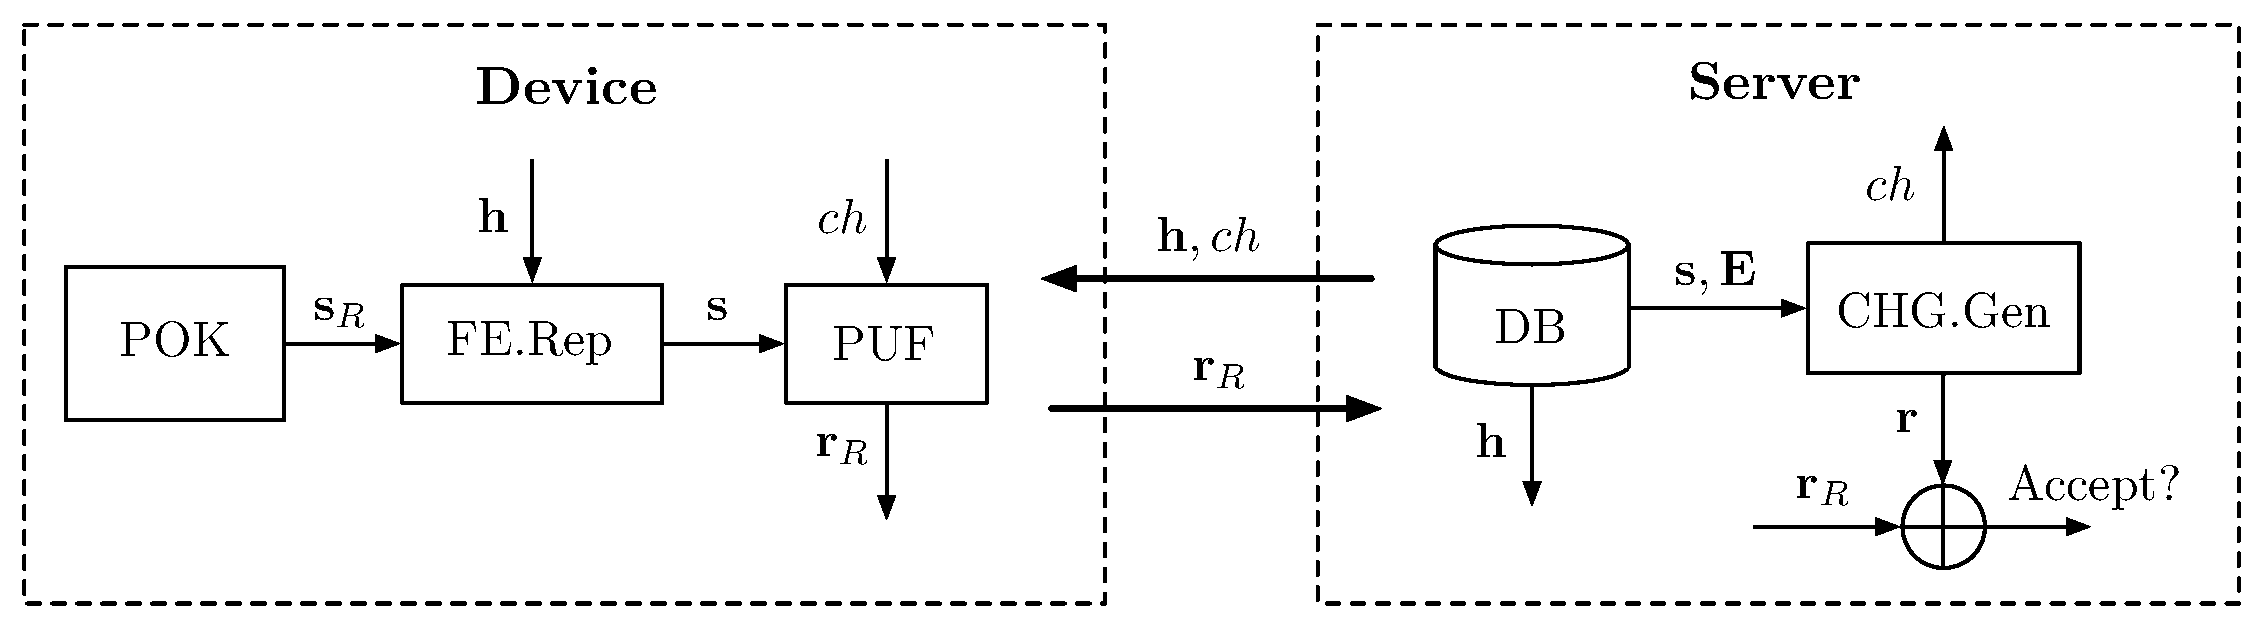
\includegraphics[width = 1.0\linewidth]{./figs/authen_system}
% \caption{Building blocks of the authentication scheme with the lattice PUF.}
% \label{fig:authen_system}
% \end{figure}

\begin{figure}[t!]
\centering
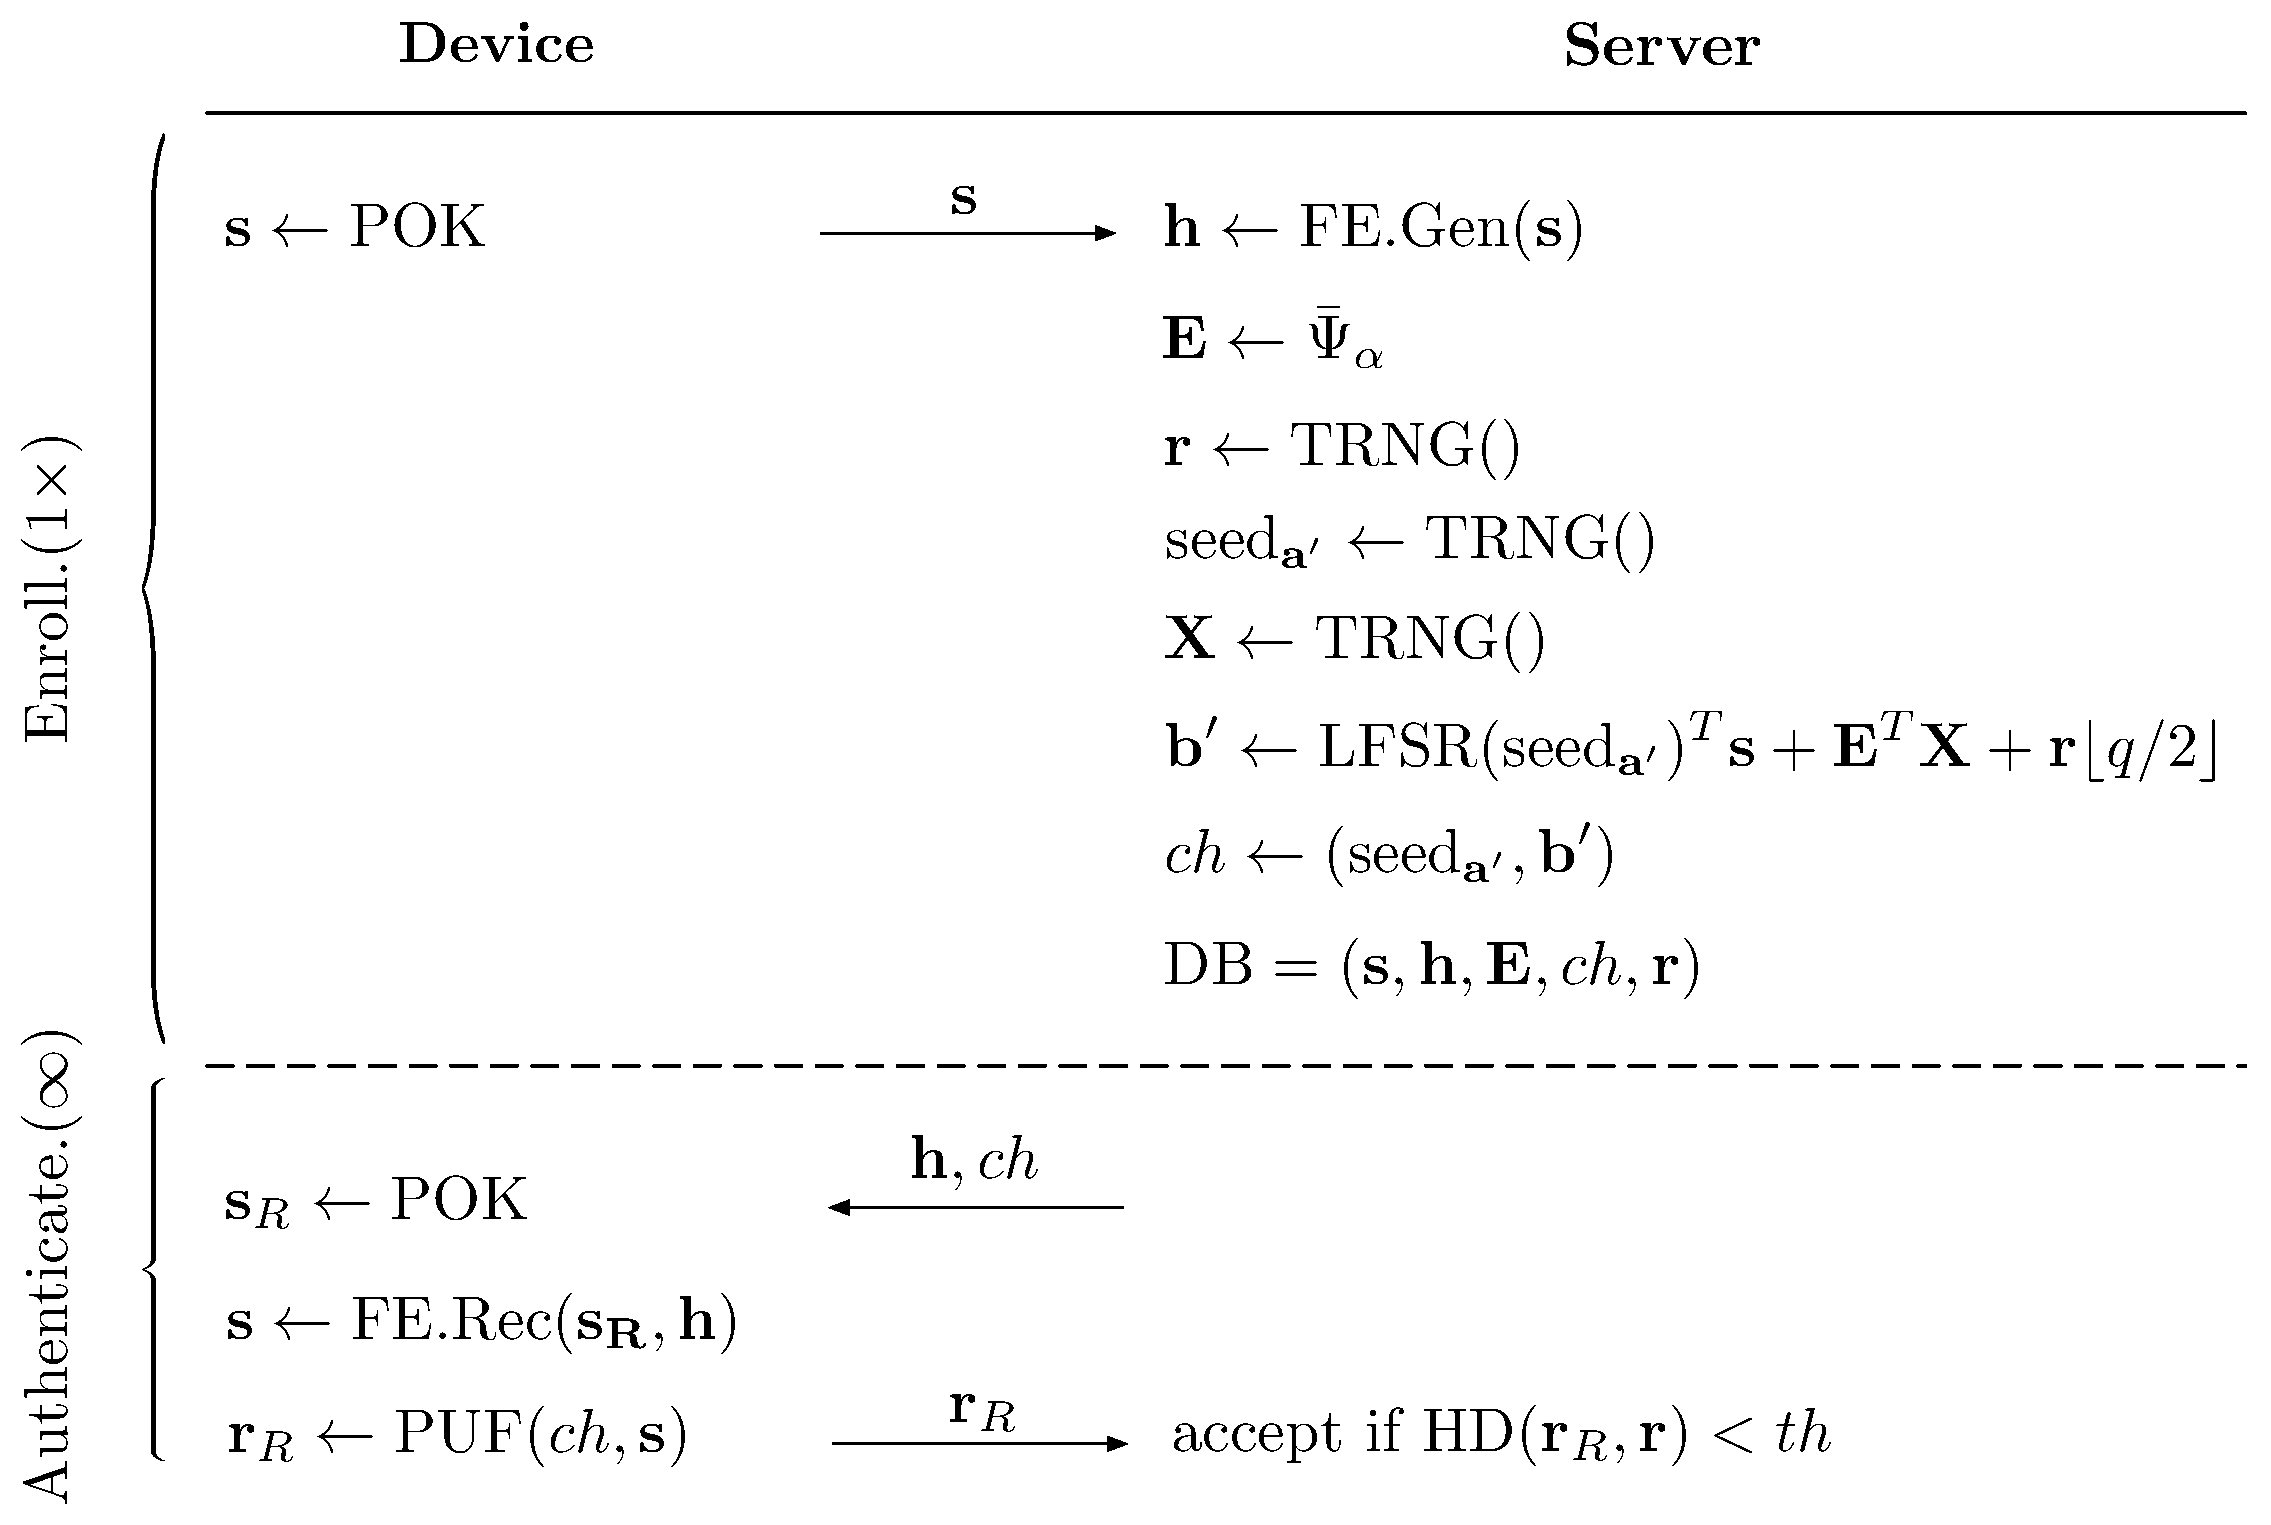
\includegraphics[width = 1.0\linewidth]{./figs/protocol}
\caption{End-to-end authentication method with the lattice PUF.}
\label{fig:protocol}
\end{figure}

\subsection{PUF-Based Authentication}
As an example application, we study using the lattice PUF in a string-matching authentication scheme \cite{suh2007physical}. 
To reconstruct the same secret key from POK bits each time, we adopt the fuzzy extractor (FE) \cite{bosch2008efficient} method to achieve a low failure rate. 
Figure \ref{fig:protocol} shows the operations of an end-to-end authentication method using the lattice PUF. 

% Figure \ref{fig:authen_system} shows the building blocks of an authentication scheme based on the lattice PUF. 
% The device contains a POK generator, an FE block (\texttt{FE.Gen} and \texttt{FE.Rec}), and a lattice PUF. 
% The server has a database (\texttt{DB}) to store the secret key from the lattice PUF and the valid CRPs generated from enrollment phase.
% Our threat model assumes that the device operates in the field and is the target of ML attacks. 
% %We consider the server to be in a physically secure location, with the \texttt{DB} storing the POK bits and the sever-side lattice PUF being secret. 

During the enrollment phase, the server reads out the power-up values of SRAM cells through a one-time interface, runs the helper data generation block in FE \texttt{FE.Gen} (for subsequent reconstructions), and stores both secret key $\mathbf{s}$ and helper data $\mathbf{h}$ in the server \texttt{DB}.
Note that there is a critical difference between the PUF and the public key cryptosystem use-cases:
for applications using public key cryptosystem, there is only an insecure public channel assumed,
while for applications using PUFs, secret information can be transferred in a secure manner.
Since only a public key can be transferred, for a direct implementation of the LWE cryptosystem, the device side has to perform the public key generation including the relatively expensive discrete Gaussian sampling. 
With $\mathbf{s}$ securely transferred to the server side in PUF enrollment phase, the computationally expensive discrete Gaussian sampling ($\mathbf{e}$) can happen on the server side rather than the PUF side.
Moreover, keeping $\mathbf{s}$ on the server side also enables challenge compression via dimension relaxation. 
Upon receiving the secret $\mathbf{s}$, the server performs CRP generation and stores them, as shown in Figure \ref{fig:protocol}.

During each authentication, the error correction uses the decoder of a concatenated code. 
If the HD between $\mathbf{s}$ and $\mathbf{s}_R$ is within the error-decoding capability of the error correction code (ECC) decoder, the device reconstructs the correct secret key $\mathbf{s}$ with the helper data. 
Finally, the server sends the valid challenge $ch=(\text{seed}_{\mathbf{a}^\prime}, \mathbf{b}')$ to the device. 
The device generates the PUF response $\mathbf{r}_R$ by running the PUF function $\mathbf{r}_R = \text{PUF}(ch, \mathbf{s})$ and sends it to the server. 
The server compares $\mathbf{r}_R$ with the response $\mathbf{r}$ stored in DB:
the device is accepted if $\text{HD}(\mathbf{r}_R, \mathbf{r})$ is less than a given threshold $th$.

\section{Experimental Results}
\label{sec:result}

We simulate the behavior of the proposed ML-resistant PUF using Python. The statistics of raw SRAM PUF responses are based on \cite{maes2013accurate, maes2009soft}. The logical behavior of other digital circuits are accurately captured by software. We virtually manufacture (simulate) $1000$ distinct lattice PUF instances with design parameters chosen in Section \ref{sec:design}. The CRPs of the PUF instances are collected to examine: (1) statistical characteristics (uniformity, uniqueness, and reliability), and (2) resistance to leading ML modeling attacks. The whole lattice PUF design (besides the SRAM PUF) is implemented on a Xilinx Spartan-6 FPGA.


\subsection{Statistical Analysis}
\label{sec:statistical_result}
%\textbf{Uniformity} of a PUF characterizes unbiasedness, namely, the proportion of `0's and `1's in the output responses.
%For an ideal PUF $f$, the proportion needs to be $50\%$ for either `0' or `1'.
%Uniformity is formally defined as the average Hamming weight $\HW(f)$ of responses $\mathbf{r}$ over randomly sampled challenges $\mathbf{c}$'s \cite{maiti2013systematic}:
%\begin{equation*}
%\HW(f)= \Expect_\mathbf{c}[\HW(\mathbf{r})] = \Expect_{\mathbf{c}}[\HW(f(\mathbf{c}))].
%\end{equation*}
%Here $\Expect_X$ represents expectation over random variable $X$.
%Note that $\mathbf{c}$ follows the ciphertext distribution rather than the usual uniform distribution \cite{maiti2013systematic}.
%Figure \ref{fig:HW} shows uniformity obtained using $1000$ randomly selected challenges. 
%The distribution is centered at $49.98\%$, the standard deviation is $1.58\%$. 


%\textbf{Uniqueness} measures the ability of a PUF to be uniquely distinguished among a set of PUFs. 
%Based on \cite{maiti2013systematic}, we define this metric to be the average inter-class HD of responses $(\mathbf{r}_i,\mathbf{r}_j)$ under the same challenges $\mathbf{c}$ for a randomly picked PUF pair $(f_i, f_j)$:
%\begin{equation*}
%\HD(f_i,f_j) = \Expect_\mathbf{c}[\HD(\mathbf{r}_i,\mathbf{r}_j)]=\Expect_{\mathbf{c}}[\HD(f_i(\mathbf{c}),f_j(\mathbf{c}))].
%\end{equation*}
%For ideal PUFs, responses under the same challenges are orthogonal, namely, $\HD(f_i,f_j)$'s are close to $50\%$.
%Uniqueness is also evaluated under the ciphertext distribution.  

%Uniqueness is shown in Figure \ref{fig:inter_intra}, evaluated for $1000$ PUF instances. 
%The lattice PUF achieves near-optimal uniqueness: inter-class HD is centered at $50.00\%$, its standard deviation is $1.58\%$. 

%\textbf{Reliability} of a PUF $f$ is characterized by the average BER of outputs with respect to their enrollment values:
%\begin{equation*}
%\BER = \Expect_{f^\prime}[\HD(f,f^\prime)]= \Expect_{f^\prime,\mathbf{c}}[\HD(f(\mathbf{c}),f^\prime(\mathbf{c}))].
%\end{equation*}
%As discussed in Section \ref{sec:design}, the overall BER of the lattice PUF is due to two components: the failure rate of key reconstruction and LWE decryption error rate.
%Intra-class HD in Figure \ref{fig:inter_intra} reflects the result of decryption errors by assuming a perfect key reconstruction. 

In this section, we examine statistical metrics of the proposed PUF. Uniformity, uniqueness and reliability are commonly adopted metrics to evaluate the statistical performance of a PUF \cite{maiti2013systematic}. \textbf{Uniformity} measures the mean Hamming Weight of responses from a PUF under a set of random challenges. The ideal uniformity is 0.5, which indicates the zero bits and the one bits are distributed uniformly in PUF response. \textbf{Uniqueness} measures the mean Hamming Distance of PUF responses between a pair of different PUF instances (inter-class HD), with the same set of PUF challenges. The ideal uniqueness is 0.5, which means each PUF instance produces a unique response distribution. \textbf{Reliability} measures the mean Hamming Distance between actual PUF responses and the enrolled (ideal) PUF responses (intra-class HD). The ideal PUF is expected to have no bit flips in responses compared to the enrolled values.

We evaluate the metrics with 1000 lattice PUF instances and 1000 random challenges following LWE ciphertext distribution \cite{maiti2013systematic}. The lattice PUF demonstrates near ideal statistical properties: the mean of uniformity distribution is 0.4998 (std = 0.0158) and the mean of uniqueness distribution is 0.5 (std = 0.0158). To evaluate PUF reliability, we assume the key reconstruction process is ideal and the errors merely come from LWE decryption. Figure \ref{fig:inter_intra} shows the lattice PUF reliability distribution centers close to 0. 



%\begin{figure}[t!]
%\centering
%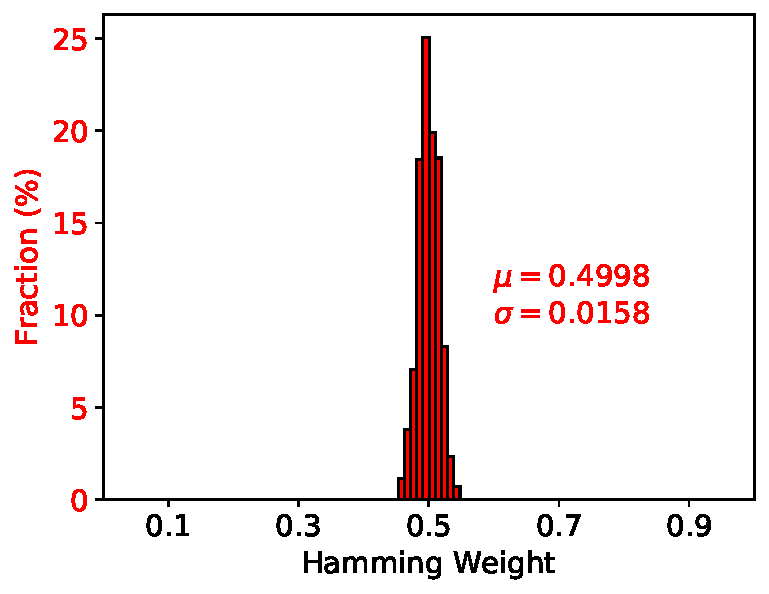
\includegraphics[width = 0.7\linewidth]{./figs/HW.pdf}
%\caption{Uniformity of lattice PUF output.}
%\label{fig:HW}
%\end{figure}

%\begin{figure}[t!]
%\centering
%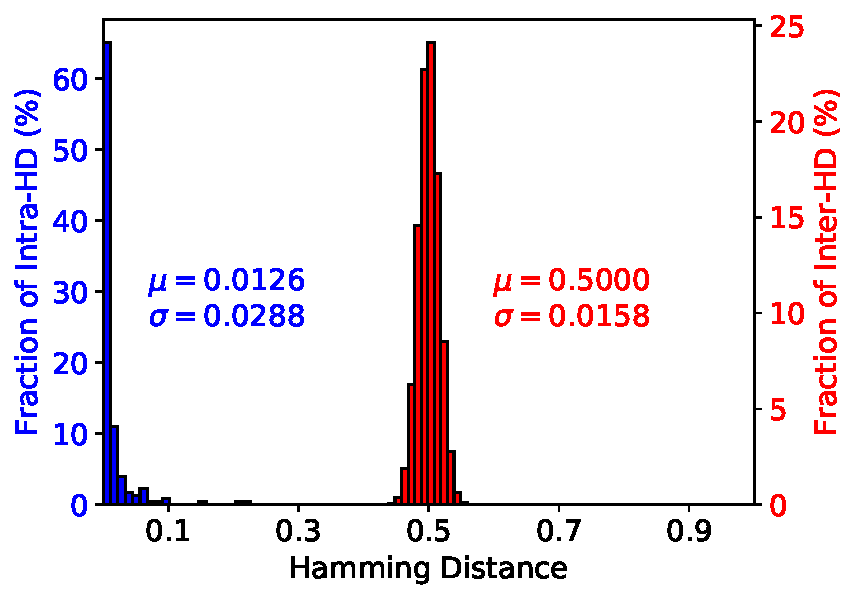
\includegraphics[width = 0.75\linewidth]{./figs/inter_intra.pdf}
%\caption{Uniqueness and reliability of lattice PUF output.}
%\label{fig:inter_intra}
%\end{figure}

\begin{figure} 
    \centering
  \subfloat[\label{fig:HW}]{%
       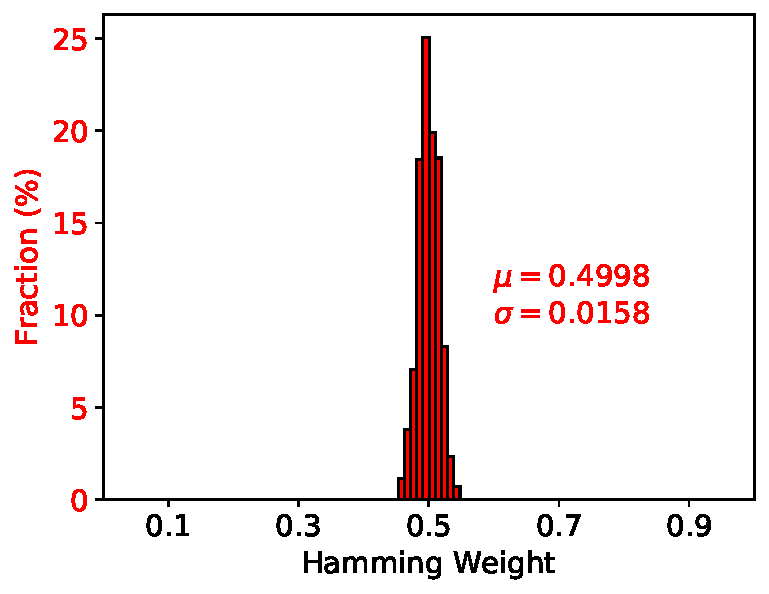
\includegraphics[width=0.45\linewidth]{./figs/HW.pdf}}
    \hfill
  \subfloat[\label{fig:inter_intra}]{%
        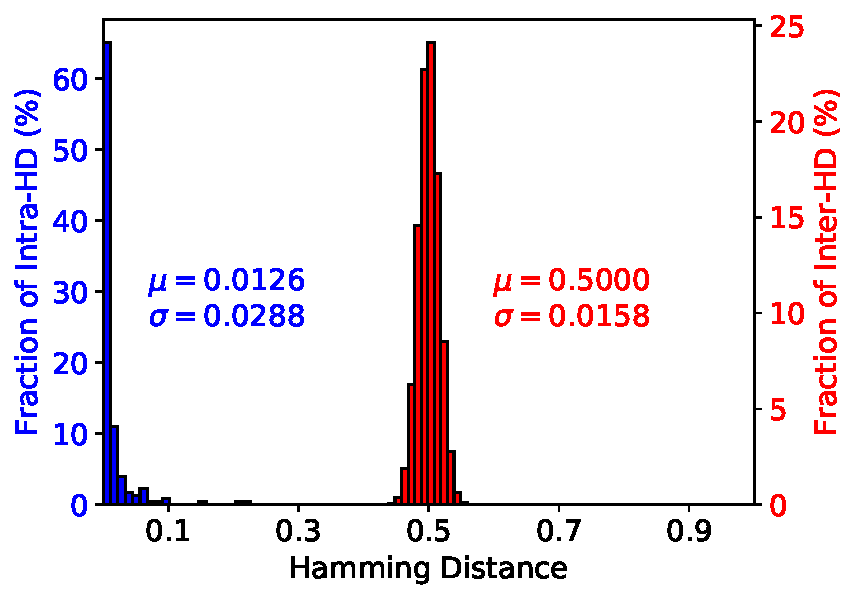
\includegraphics[width=0.5\linewidth]{./figs/inter_intra.pdf}}
  \caption{(a) Lattice PUF has near ideal uniformity. (b) Lattice PUF has near ideal uniqueness and reliability.}
  \label{fig: lattice_puf_stats} 
\end{figure}

%\begin{figure}[t!]
%\centering
%\begin{subfigure}{0.2\textwidth}
%   \centering
%   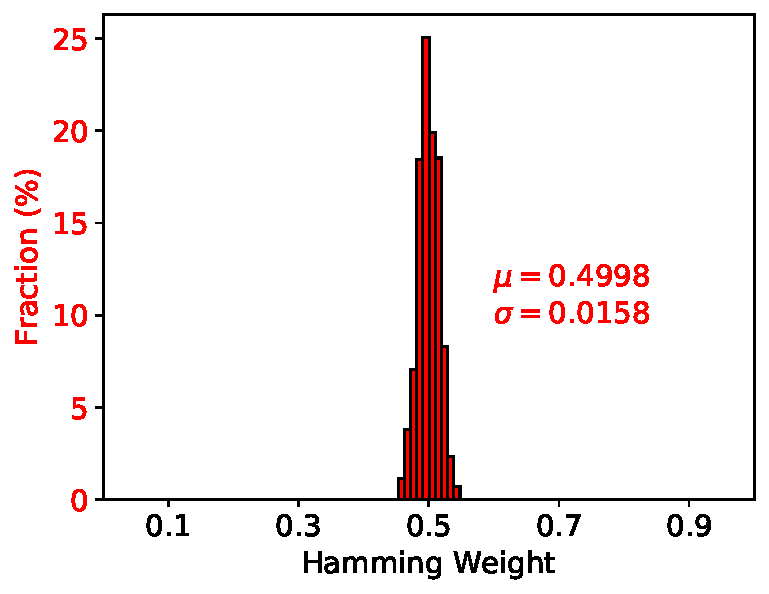
\includegraphics[width=\textwidth]{./figs/HW.pdf}
   %\caption{Uniformity of lattice PUF output.}
%   \label{fig:HW} 
%\end{subfigure}
%\begin{subfigure}{0.24\textwidth}
%   \centering
%   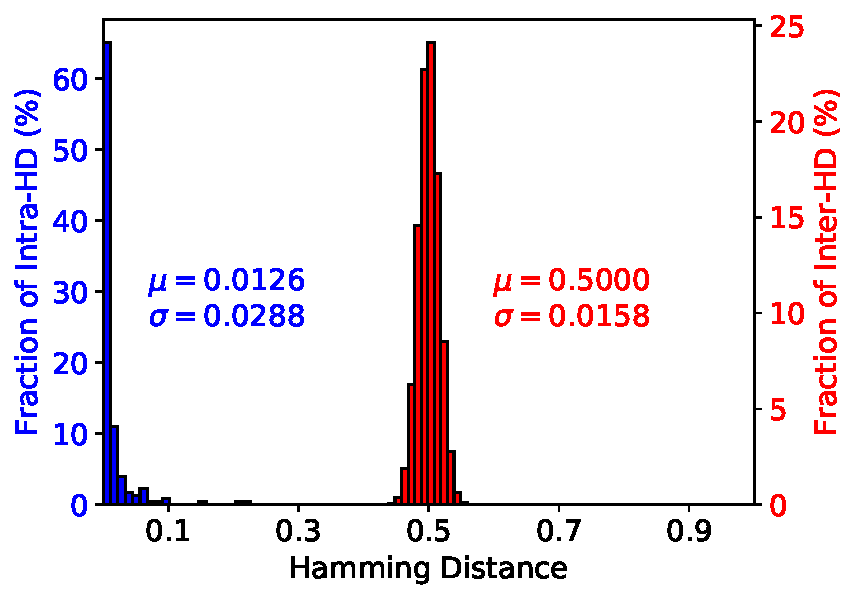
\includegraphics[width=\textwidth]{./figs/inter_intra.pdf}
   %\caption{Uniqueness and reliability of lattice PUF output.}
%   \label{fig:inter_intra}
%\end{subfigure}
%\caption{(a) Uniformity of lattice PUF output. (b) Uniqueness and reliability of lattice PUF output.}
%\label{power_trace_avg_untrusted_devices_1_to_15}
%\end{figure}

\subsection{ML Attacks on Lattice PUF}

%While the ultimate promise of lattice PUF is due to its theoretically-supported reliance on hard computational problems,
%testing its ML resistance empirically gives a concrete measure of its security. The resistance of lattice PUF is evaluated with a series of traditional (i.e., not based on deep learning) ML algorithms, including SVM, LR, and single-layer NN (1-NN), as well as a number of DNNs.
%We use the Python scikit-learn %\cite{scikit-learn} 
%package to implement SVM and LR.  
%The SVM uses the radial basis function (RBF) kernel.
%The 1-NN model uses only one hidden feed-forward layer composed of 100 neurons, with the rectified linear unit (ReLU) as the activation function. 
%Training of 1-NNs and subsequent DNNs are implemented using Keras %\cite{chollet2015keras} 
%with TensorFlow %\cite{abadi2016tensorflow} 
%backend.

Although we establish the security of lattice PUF theoretically, we perform empirical validation as a way to explore the possible attacks of distributional relaxations used, and as a way to give added overall confidence in the design. The traditional ML algorithms include LR, SVM and one-layer Neural Network (1-NN). The LR and SVM are implemented with scikit-learn package in Python. We use the RBF kernel in SVM, which models a non-linear decision boundary. The single hidden layer of 1-NN consists of 100 neurons, and the activation function is selected to be ReLU. We train the 1-NN and DNNs with Keras powered by Tensorflow.


\begin{figure}[t!]
\centering
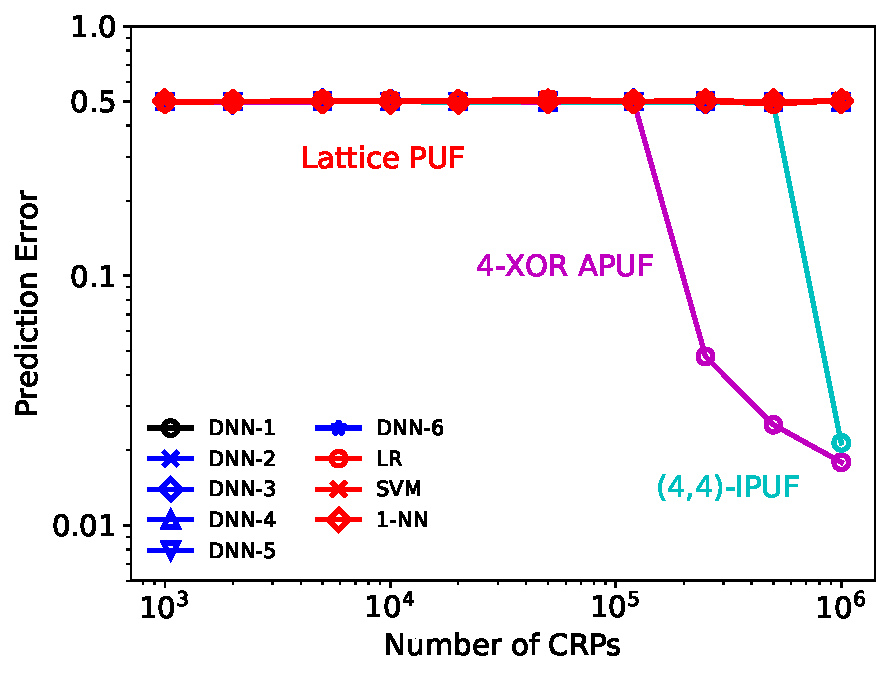
\includegraphics[width = 0.7\linewidth]{./figs/ml_attack_dnn_all_puf_5_new.pdf}
\caption{Lattice PUF is resilient to multiple ML modeling attacks including DNNs. Two other strong PUFs are ultimately vulnerable to DNN-based attacks.}
\label{fig:ml_attack_2}
\end{figure}

\begin{figure}[t!]
\centering
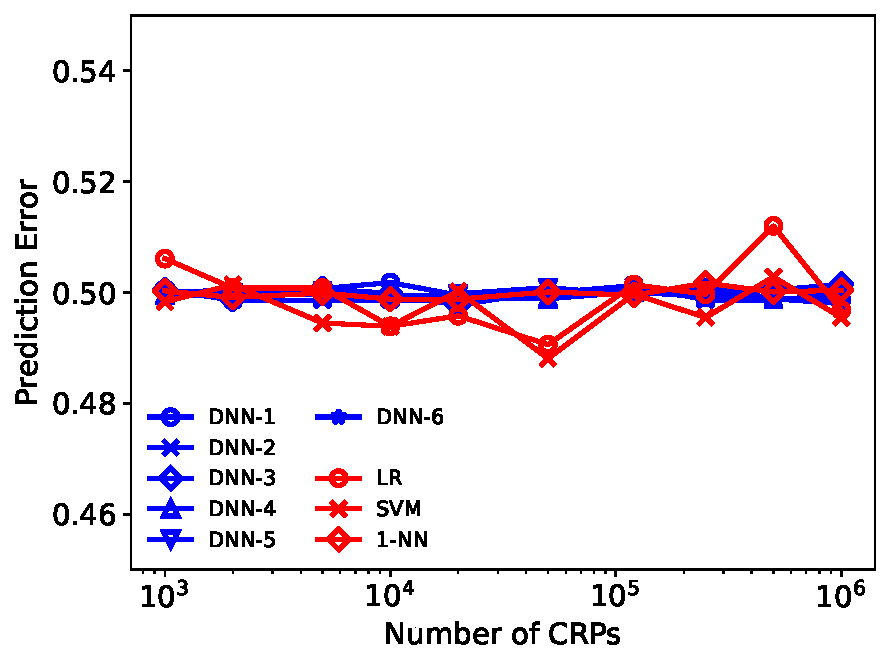
\includegraphics[width = 0.7\linewidth]{./figs/ml_attack_lattice_puf_new.pdf}
\caption{Lattice PUF can not be broken by both conventional ML algorithms and more powerful DNNs.}
\label{fig:ml_attack_3}
\end{figure}

%\begin{figure}[t!] 
%    \centering
%  \subfloat[\label{fig:ml_attack_2}]{%
%       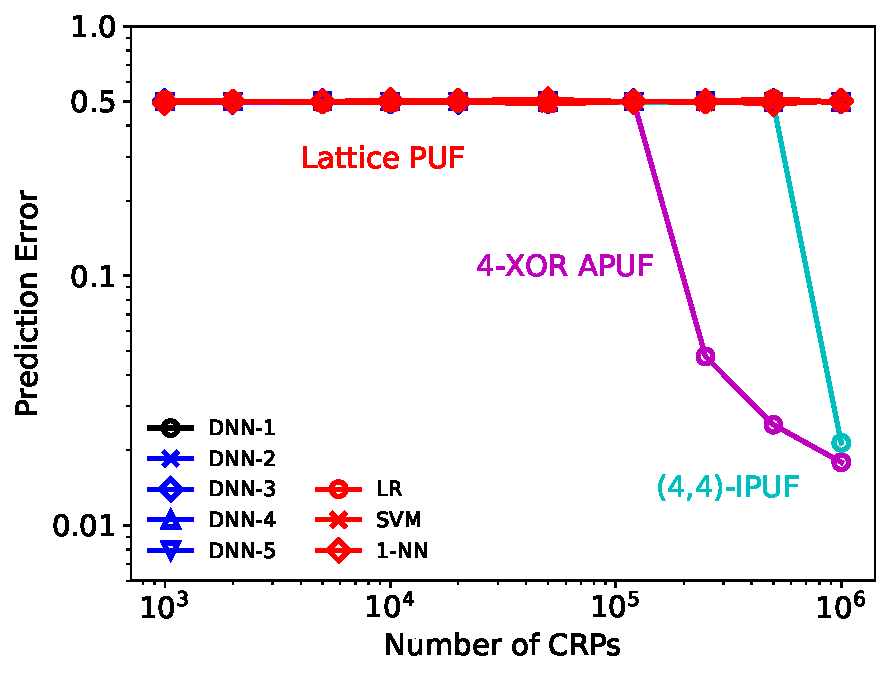
\includegraphics[width=0.5\linewidth]{./figs/ml_attack_dnn_all_puf_5.pdf}}
%    \hfill
%  \subfloat[\label{fig:ml_attack_3}]{%
%        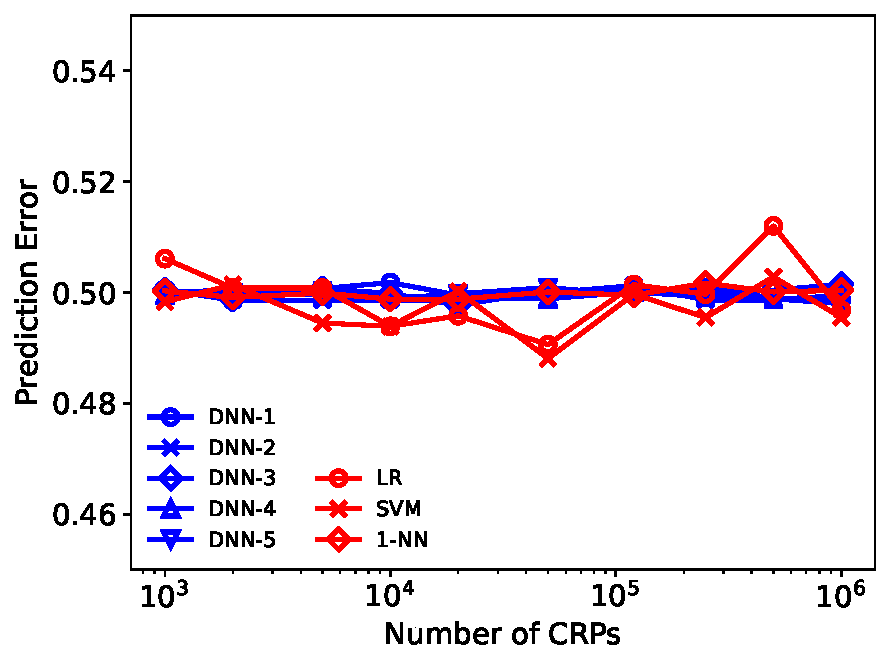
\includegraphics[width=0.5\linewidth]{./figs/ml_attack_lattice_puf.pdf}}
%  \caption{(a) ML attacks: Lattice PUF remains resistant to all attacks (DNNs, LR, SVM,1-NN). DNN ultimately succeeds in modeling two other strong PUFs. (b) Lattice PUF is resistant to both traditional ML attacks and DNNs.}
%  \label{fig: lattice_puf_ml_attack_results} 
%\end{figure}

\begin{table}[t!]
\centering
	%\caption{Different DNN configurations in modeling attacks.}
	%\label{table:DNNSetting}
	\resizebox{\linewidth}{!}{
        \begin{tabular}{|c|c|c|c|c|c|}
        \hline
        \textbf{Setup} & \begin{tabular}[c]{@{}l@{}}\textbf{Hidden}\\ \textbf{Layers}\end{tabular} & \begin{tabular}[c]{@{}c@{}}\textbf{Neurons}\\ \textbf{per Layer}\end{tabular} & \begin{tabular}[c]{@{}c@{}}\textbf{Challenge} \\ \textbf{Distribution}\end{tabular} & \begin{tabular}[c]{@{}c@{}}\textbf{Input} \\ \textbf{Format}\end{tabular} & \begin{tabular}[c]{@{}c@{}}\textbf{Prediction}\\ \textbf{Error}\end{tabular} \\ \hline
        DNN-1     & 4                                                       & 100                                                         & PRNG                                                              & Binary                                                  & 49.86\%                                                       \\ \hline
        DNN-2     & 4                                                       & 100                                                         & PRNG                                                              & Real                                                    & 49.84\%                                                       \\ \hline
        DNN-3     & 4                                                       & 100                                                         & Ciphertext                                                        & Binary                                                  & 49.76\%                                                       \\ \hline
        DNN-4     & 6                                                       & 100                                                         & PRNG                                                              & Binary                                                  & 49.80\%                                                       \\ \hline
        DNN-5     & 4                                                       & 200                                                         & PRNG                                                              & Binary                                                  & 49.87\%                                                       \\ \hline
        DNN-6     & 12                                                       & 2000                                                         & PRNG                                                              & Binary                                                  &    49.95\%                                                    \\ \hline
        \end{tabular}
    }
    \vspace{1em}
    \caption{Different DNN configurations in modeling attacks.}
    \label{table:DNNSetting}
    \vspace{-2em}
\end{table}

%DNNs are more powerful in binary classification. DNNs contain multiple hidden layers which enable superior modeling expressiveness compared to 1-NNs \cite{goodfellow2016deep}. Notably, recent successful DNN-based attacks have been demonstrated on published strong PUFs, including XOR APUFs and IPUFs \cite{DBLP:journals/iacr/SantikellurBC19}. Our baseline DNN experiment (DNN-1) adopts the same network parameters as in \cite{DBLP:journals/iacr/SantikellurBC19}.  The network has 4 hidden layers, each containing 100 neurons. It uses ReLU as the non-linear operator. 

DNN is a class of ML algorithms often highly effective in classification tasks. 
Its superior performance against 1-NNs is enabled by the expressiveness of multiple hidden neuron layers. Notably, recent successful DNN-based attacks have been demonstrated on strong PUFs, such as IPUFs \cite{DBLP:journals/iacr/SantikellurBC19},  XOR APUFs \cite{DBLP:journals/iacr/SantikellurBC19} and XOR BR PUFs \cite{dnn_xor_br_puf}. We select the DNN parameters in \cite{DBLP:journals/iacr/SantikellurBC19} as our baseline configuration (DNN-1): the number of hidden layers is 4, the number of neurons per layer is 100, and the activation function is ReLU.  

%Besides the parameters used in the baseline experiment, we varied network architectures, hyper-parameters, and numeric representations in the attack, as listed in Table \ref{table:DNNSetting}. 
%DNN-2 treats input as 161 integer numbers from 0 to 255, instead of 1288 binary bits.
%DNN-3 is different from the baseline version in its CRP generation strategy (see more below).
%DNN-4 and DNN-5 add more hidden layers and more neurons per hidden layer respectively, compared to the baseline DNN-1.

We explored multiple DNN configurations beyond the baseline experiment, Table \ref{table:DNNSetting}. The input to DNN-2 concatenates 161 8-bit integers. The input to DNN-3 follows a different challenge distribution. DNN-4 has an increased number of hidden layers and DNN-5 has an increased number of neurons within each layer. DNN-6 follows the configuration of a recent attack on XOR BR PUFs \cite{dnn_xor_br_puf}, and has a much larger number of both hidden layers and neurons per layer.

%Figure \ref{fig:ml_attack_2} shows the results of the empirical attacks based on the above ML algorithms. The figure shows the prediction error of lattice PUF in response to these attacks with training set size ranging from $1000$ to $1$ million and test set of size $200$K. The Adam optimizer \cite{kingma2014adam} terminates after 200 epochs, and results in a prediction error of $49.86\%$, barely better than a random guess. \emph{The results show that the prediction error of lattice PUF remains flat for all attempted attacks: across the range of attacks and CRP training set sizes, there is no measurable deviation of the error from 0.5.} In contrast, a DNN (with a configuration corresponding to DNN-1) achieves less than $2\%$ prediction error for both 4-XOR APUF and (4, 4)-IPUF.

The lattice PUF again demonstrates near perfect empirical ML resistance, Figure \ref{fig:ml_attack_2}. The results are reported using a test set with 200K CRPs and the DNNs are trained with the Adam optimizer running for 200 epochs. Regardless of the algorithms and the number of training CRPs used in the attack, the prediction error remains close to 0.5, which is equivalent to a random coin-flip. However, the two other strong PUFs can be successfully modelled by DNNs, with a prediction error smaller than 2\%.

%It is important to note that the experiments also show that the use of distributional relaxation of space-efficient LWE (described in Section \ref{sec:lfsr}) does not hinder empirical ML resistance of lattice PUF. In Table 1, all design/attack combinations except for DNN-3 are based on the compact (relaxation-based) design in which CRPs are generated via a PRNG. Finally, we show a detailed view of ML attack results on lattice PUF in Figure \ref{fig:ml_attack_3} by zooming in Figure \ref{fig:ml_attack_2}. While run-to-run variations of the training optimizer are observable, the prediction error remains close to $50\%$.

The results also validate the challenge compression technique demonstrated in Section \ref{sec:lfsr}. The DNN-1, DNN-2, DNN-4, DNN-5, and DNN-6 adopt challenges produced by the PRNG, but still show a prediction error close to 0.5. Figure \ref{fig:ml_attack_3} shows a zoomed view of DNN attack results on lattice PUF.

\subsection{Hardware Implementation Results}
\label{sec:hardware_results}

In this section, we show the hardware implementation details of lattice PUF. We synthesize, configure and test the entire design on a low-end XC6SLX45 FPGA device of Xilinx Spartan-6 family.  

We adopt the homogeneous error assumption regarding the RFE design. This means all cells are assumed to have the same BER \cite{bosch2008efficient}.
The BER of different POKs varies from $0.1\%$ \cite{karpinskyy20168} to $15\%$ \cite{maes2009soft}.
We configure BER = $1\%$, BER = $5\%$, BER = $10\%$ and BER = $15\%$ to investigate design trade-offs in RFE and POK, and finally configure the BER of SRAM POK in our design to be $5\%$. The RFE targets a $10^{-6}$ failure rate in reconstruction of $1280$ key bits. 
As described in Section \ref{sec:design}, the overall lattice PUF response BER can achieve the desired value with such a low key reconstruction failure rate.
Our ECC concatenates an inner code and an outer code. The inner code adopts repetition code and the outer code adopts shortened BCH code. Concatenated ECCs usually have shorter code length and lower hardware cost, compared to single codes \cite{bosch2008efficient}.
As described in Section \ref{sec:design}, the RFE scheme needs only lightweight encoder implementation on the device side. 
Table \ref{table:ecc} and \ref{table:hardware_fe} show the parameters and hardware utilization of ECCs with different configurations for BER.
A $5\%$ BER value requires $6.36K$ SRAM cells in order to reconstruct the $1280$-bit secret value $\mathbf{s}$ with a failure rate of $10^{-6}$.
The RFE encoder design requires $26$ slices. 
We adopt the SRAM-based design of \cite{aysu2015end} to implement the TRNG. The advantage is that the SRAM cells used to generate $\mathbf{s}$ can be reused for the SRAM-TRNG design. 
We adopt the 8-fold XORing of SRAM bits in \cite{aysu2015end} and therefore need $10.06K$ (i.e. $3.7K$ additional) SRAM cells. 
The 8-fold XORing logic design requires $1$ slice. 
Then, for the $5\%$ raw BER, the RFE design requires $27$ slices in total. 


%\begin{table}[t!]
%\centering
%\caption{Latency of different lattice PUF designs for 128-bit response generation [$\mu$s]. $P_1$ denotes number of LFSR-LWEDec data-paths; $P_2$ denotes number of LFSR output bits.} 
%\label{table:latency_par}
%\begin{tabular}{cccccccc}
%\hline
%\multicolumn{1}{|l|}{}            & \multicolumn{7}{c|}{\textbf{$\mathbf{P_2}$}}                                                                                                                                                                                                                 \\ \hline
%\multicolumn{1}{|c|}{\textbf{$\mathbf{P_1}$}} & \multicolumn{1}{c|}{\textbf{1}} & \multicolumn{1}{c|}{\textbf{4}} & \multicolumn{1}{c|}{\textbf{8}} & \multicolumn{1}{c|}{\textbf{16}} & \multicolumn{1}{c|}{\textbf{32}} & \multicolumn{1}{l|}{\textbf{64}} & \multicolumn{1}{l|}{\textbf{128}} \\ \hline
%\multicolumn{1}{|c|}{\textbf{1}}  & \multicolumn{1}{c|}{5632}       & \multicolumn{1}{c|}{1843}       & \multicolumn{1}{c|}{1229}       & \multicolumn{1}{c|}{614}         & \multicolumn{1}{c|}{307}         & \multicolumn{1}{c|}{154}         & \multicolumn{1}{c|}{77}           \\ \hline
%\multicolumn{1}{|c|}{\textbf{2}}  & \multicolumn{1}{c|}{2765}       & \multicolumn{1}{c|}{922}        & \multicolumn{1}{c|}{614}        & \multicolumn{1}{c|}{307}         & \multicolumn{1}{c|}{154}         & \multicolumn{1}{c|}{77}          & \multicolumn{1}{c|}{38}           \\ \hline
%\multicolumn{1}{|c|}{\textbf{4}}  & \multicolumn{1}{c|}{1382}       & \multicolumn{1}{c|}{461}        & \multicolumn{1}{c|}{307}        & \multicolumn{1}{c|}{154}         & \multicolumn{1}{c|}{77}          & \multicolumn{1}{c|}{38}          & \multicolumn{1}{c|}{NA}           \\ \hline
%\multicolumn{1}{|c|}{\textbf{8}}  & \multicolumn{1}{c|}{691}        & \multicolumn{1}{c|}{230}        & \multicolumn{1}{c|}{154}        & \multicolumn{1}{c|}{77}          & \multicolumn{1}{c|}{38}          & \multicolumn{1}{c|}{NA}          & \multicolumn{1}{c|}{NA}           \\ \hline
%\multicolumn{1}{l}{}              & \multicolumn{1}{l}{}            & \multicolumn{1}{l}{}            & \multicolumn{1}{l}{}            & \multicolumn{1}{l}{}             & \multicolumn{1}{l}{}             & \multicolumn{1}{l}{}             & \multicolumn{1}{l}{}              \\
%\multicolumn{1}{l}{}              & \multicolumn{1}{l}{}            & \multicolumn{1}{l}{}            & \multicolumn{1}{l}{}            & \multicolumn{1}{l}{}             & \multicolumn{1}{l}{}             & \multicolumn{1}{l}{}             & \multicolumn{1}{l}{}             
%\end{tabular}
%\end{table}
                          

%\begin{table}[t!]
%\centering
%\caption{Hardware utilization of different lattice PUF designs [slices]. $P_1$ denotes number of LFSR-LWEDec data-paths; $P_2$ denotes number of LFSR output bits.}
%\label{table:hwslices_par}
%\begin{tabular}{cccccccc}
%\hline
%\multicolumn{1}{|l|}{}            & \multicolumn{7}{c|}{\textbf{$\mathbf{P_2}$}}                                                                                                                                                                                                                 \\ \hline
%\multicolumn{1}{|c|}{\textbf{$\mathbf{P_1}$}} & \multicolumn{1}{c|}{\textbf{1}} & \multicolumn{1}{c|}{\textbf{4}} & \multicolumn{1}{c|}{\textbf{8}} & \multicolumn{1}{c|}{\textbf{16}} & \multicolumn{1}{c|}{\textbf{32}} & \multicolumn{1}{l|}{\textbf{64}} & \multicolumn{1}{l|}{\textbf{128}} \\ \hline
%\multicolumn{1}{|c|}{\textbf{1}}  & \multicolumn{1}{c|}{45}         & \multicolumn{1}{c|}{123}        & \multicolumn{1}{c|}{124}        & \multicolumn{1}{c|}{137}         & \multicolumn{1}{c|}{150}         & \multicolumn{1}{c|}{178}         & \multicolumn{1}{c|}{287}          \\ \hline
%\multicolumn{1}{|c|}{\textbf{2}}  & \multicolumn{1}{c|}{249}        & \multicolumn{1}{c|}{298}        & \multicolumn{1}{c|}{301}        & \multicolumn{1}{c|}{320}         & \multicolumn{1}{c|}{373}         & \multicolumn{1}{c|}{362}         & \multicolumn{1}{c|}{465}          \\ \hline
%\multicolumn{1}{|c|}{\textbf{4}}  & \multicolumn{1}{c|}{348}        & \multicolumn{1}{c|}{463}        & \multicolumn{1}{c|}{463}        & \multicolumn{1}{c|}{546}         & \multicolumn{1}{c|}{629}         & \multicolumn{1}{c|}{631}         & \multicolumn{1}{c|}{NA}           \\ \hline
%\multicolumn{1}{|c|}{\textbf{8}}  & \multicolumn{1}{c|}{561}        & \multicolumn{1}{c|}{834}        & \multicolumn{1}{c|}{847}        & \multicolumn{1}{c|}{920}         & \multicolumn{1}{c|}{1015}        & \multicolumn{1}{c|}{NA}          & \multicolumn{1}{c|}{NA}           \\ \hline
%\multicolumn{1}{l}{}              & \multicolumn{1}{l}{}            & \multicolumn{1}{l}{}            & \multicolumn{1}{l}{}            & \multicolumn{1}{l}{}             & \multicolumn{1}{l}{}             & \multicolumn{1}{l}{}             & \multicolumn{1}{l}{}              \\
%\multicolumn{1}{l}{}              & \multicolumn{1}{l}{}            & \multicolumn{1}{l}{}            & \multicolumn{1}{l}{}            & \multicolumn{1}{l}{}             & \multicolumn{1}{l}{}             & \multicolumn{1}{l}{}             & \multicolumn{1}{l}{}             
%\end{tabular}
%\end{table}


% \begin{figure}[t!]
% \centering
% 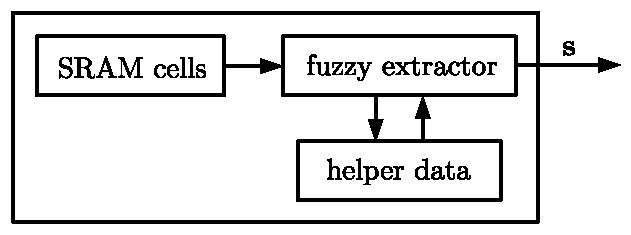
\includegraphics[width = 0.75\linewidth]{./figs/pok.pdf}
% \caption{POK uses an FE to ensure stability of the secret seed.}
% \label{fig:pok}
% \end{figure}

%We now present the details of implementing the lattice PUF, as shown in Figure \ref{fig:fpga_impl}. 
%In this section, we show the hardware implementation details of lattice PUF. The entire design, except for the raw (uninitialized) SRAM cells, was synthesized, configured, and tested on a Xilinx Spartan-6 FPGA (XC6SLX45), a low-end FPGA in 45nm technology.

%The cost of FE/RFE applies to all other strong PUF candidates (AES PUF or other controlled PUF).
%This is also cheaper than linear solver block used in the CFE-based strong PUF \cite{herder2017trapdoor,jin2017fpga} for key reconstruction, which requires $65,700$ LUTs and $16,425$ slices.

The lattice PUF (without RFE) takes a total of 45 slices on Spartan-6 FPGA. The LFSR and the controller occupies most of the slices. Table %\ref{table:fpga_utilization}
\ref{table:fpga_result}(a) shows the resources breakdown of each module. The decryption function of LWE (LWEDec) is implemented with MAC unit of 8 bits and a block for MAC result quantization, Figure \ref{fig:lwedec}.
RAM-based shift registers are used to implement the 256-bit LFSR. It takes $47\mu$s in total to generate a single PUF response bit under a clock running at 33.3MHz. 100 PUF response bits require about $4.4ms$ ($8\mu s + 100\times 44\mu s$) in total. Table %\ref{table:fpga_timing} 
\ref{table:fpga_result}(b) shows latency of each procedure to produce a PUF response.

\begin{table}[t!]
    %\caption{(a) Area consumption and (b) runtime of our reference lattice PUF implementation on Xilinx Spartan-6 FPGA.}
    %\label{table:fpga_result}
    \centering
    \def\arraystretch{1.1}
    \subfloat[]{
        \resizebox{0.45\linewidth}{!}{
            \begin{tabular}{|c|c|}
            \hline
            \textbf{Module}         & \textbf{Size [slices]} \\ \hline
            LFSR                    & 27            \\ \hline
            LWEDec                  & 2             \\ \hline
            Controller              & 16            \\ \hline
            \textit{Total}          & 45            \\ \hline
            \end{tabular}
            %\label{table:fpga_utilization}
        }
    }
    \hspace{1em}
    \subfloat[]{
        \resizebox{0.75\linewidth}{!}{
            \begin{tabular}{|c|c|}
            \hline
            \textbf{Step}                               & \textbf{Time [$\mu$s]} \\ \hline
            Seed $\text{seed}_{\mathbf{a}'}||t$ load for LFSR    & 8             \\ \hline
            1-bit decryption from LWEDec                  & 44            \\ \hline
            \textit{Total} @ 33 \textit{MHz}            & 52            \\ \hline
            \end{tabular}
            %\label{table:fpga_timing}
        }
    }
    \vspace{1em}
    \caption{(a) Area consumption and (b) runtime of our reference lattice PUF implementation on Xilinx Spartan-6 FPGA.}
    \label{table:fpga_result}
\end{table}

We now explore the design space of our proposed lattice PUF, starting with the resource-efficient design. We adopt the parallelization strategies proposed in Section \ref{sec: lpuf_par} and implement designs with different levels of parallelism. The latency and hardware utilization of the designs are summarized in Table \ref{table:latency_par} and \ref{table:hwslices_par}. Fig. \ref{fig:design_space_latency} and Fig. \ref{fig:design_space_hw} visualize the influence of $P_1$ and $P_2$ on latency and hardware cost. Similar to Table %\ref{table:fpga_utilization}
\ref{table:fpga_result}(a), we report the sum of slice utilization of LFSR, LWEDec and Controller modules. The maximum value of $P_2$ is $128$ due to the constraint of LFSR generator polynomial. Table entries with NA indicate the corresponding design requires more multipliers than the available DSP slices on the device. We observe that the parallelized design leads to a steady reduction in latency, at the cost of increased hardware utilization. We achieve a 148X reduction in latency in the most latency-optimized design, with a 10X increase in hardware utilization. %While both parallelization strategies demonstrate effectiveness in latency reduction, they have different efficiency in hardware utilization. 
In addition, we observe the MAC unit parallelization strategy has better hardware efficiency compared to LFSR-LWEDec datapath parallelization strategy. To achieve the same latency reduction, the design which prioritizes MAC unit parallelization requires fewer slices. For instance, to achieve the optimal $38 \mu$s latency, the design with $(P_1, P_2) = (2, 128)$ only requires $465$ slices, while the design with $(P_1, P_2) = (8, 32)$ requires $1,015$ slices. This validates our optimal strategy demonstrated in Section \ref{sec: lpuf_par}. %This seems to indicate the LFSR unrolling is always a better strategy for latency optimization. However, in reality, the LFSR cannot be unrolled by unlimited times while keeping the equivalent functionality. The LFSR generator polynomial limits the maximum unrolling times. For instance, if the 256-bit LFSR takes the XOR result of $X_{255}$, $X_{253}$, $X_{250}$ and $X_{7}$ as the feedback bit, the LFSR cannot be unrolled by over 8 times with the technique presented in Section \ref{sec: lpuf_par}, since the LSB $X_{0}$ is only 8 bits away from $X_{7}$. Therefore, in practice, the optimal strategy is to first seek parallelization via LFSR unrolling, and then parallelize the LFSR-LWEDec data-path to achieve further latency optimization once the unrolling of LFSR reaches the limit.

\begin{table}[t!]
\centering
	%\caption{Comparison of hardware utilization of various strong PUFs.}
	\vspace{-0.5em}
	%\label{table:hardware_puf}
	\def\arraystretch{1.1}
	\resizebox{\linewidth}{!}{
        \begin{tabular}{|c|c|c|c|c|c|c|}
        \hline
        \textbf{Design} & \textbf{Platform} & \begin{tabular}[c]{@{}c@{}}\textbf{PUF Logic}\\ \textbf{[Slices]}\end{tabular} & \begin{tabular}[c]{@{}c@{}@{}@{}}\textbf{Error-}\\ \textbf{Correction}\\\textbf{Code}\\ \textbf{[Slices]}\end{tabular} & \begin{tabular}[c]{@{}c@{}}\textbf{POK}\\ \textbf{[Bits]}\end{tabular} & \begin{tabular}[c]{@{}c@{}}\textbf{Response}\\ \textbf{[Bits]}\end{tabular} & \begin{tabular}[c]{@{}c@{}}\textbf{Latency}\\ \textbf{[$\mu$s]}\end{tabular} \\\hline
        POK+AES \cite{bhargava2014efficient} & Spartan 6 & 80 & 27 & 612 & 128 & 2.2\\ \hline
        Controlled PUF \cite{gassend2008controlled} & Spartan 6 & 127 & 27 & 612 & 256 & 19.1\\ \hline
        \begin{tabular}[c]{@{}c@{}}CFE-based PUF\\ \cite{herder2017trapdoor,jin2017fpga}\end{tabular} & Zynq-7000 & 9,225 & 0 & 450\tablefootnote{The POK is based on RO PUF and assumes a different BER.} & 256 & 658\tablefootnote{Zynq-7000 device typically runs faster than Spartan-6 device.}\\ \hline
        \begin{tabular}[c]{@{}c@{}}Lattice PUF\\ (resource-efficient)\end{tabular} & Spartan 6 & 45 & 26 & 6,360 & 128 & 5,632\\ \hline
        \begin{tabular}[c]{@{}c@{}}Lattice PUF\\ (latency-optimized)\end{tabular} & Spartan 6 & 465 & 26 & 6,360 & 128 & 38\\ \hline
        \end{tabular}
    }
    \vspace{1em}
    \caption{Comparison of hardware utilization of various strong PUFs.}
    \label{table:hardware_puf}
\end{table}

\begin{table}[t!]
    \centering
	%\caption{Configuration of concatenated ECCs.}
	%\vspace{-0.5em}
	%\label{table:ecc}
	\def\arraystretch{1.1}
	\resizebox{0.9\linewidth}{!}{
        \begin{tabular}{|c|c|c|c|c|c|}
        \hline
        \multirow{2}{*}{\begin{tabular}[c]{@{}c@{}}\textbf{Raw BER}\\  \textbf{(\%)}\end{tabular}} & \multicolumn{2}{c|}{\textbf{Error-Correcting Code}}                                 & \multirow{2}{*}{\textbf{Raw POKs}}  \\ \cline{2-3} 
                                                                                 & Outer code   & Inner code & \\ \hline
        1                                                                        & {[}236, 128, 14{]}  & N/A            & 2,360  \\ \hline
        5                                                                        & {[}212, 128, 11{]} & {[}3, 1, 1{]}  & 6,360  \\ \hline
        10                                                                       & {[}220, 128, 12{]} & {[}5, 1, 2{]}  & 11,000  \\ \hline
        15                                                                       & {[}244, 128, 15{]} & {[}7, 1, 3{]}  & 17,080   \\ \hline
        \end{tabular}
    }
    \vspace{1em}
    \caption{Configuration of concatenated ECCs.}
    \label{table:ecc}
\end{table}

\begin{table*}[t!]
    \centering
    %\caption{Hardware utilization in ECC encoder design on Spartan 6 FPGA.}
    %\label{table:hardware_fe}
        \begin{tabular}{|c|c|c|c|c|c|c|c|c|c|}
        \hline
        \multirow{2}{*}{\begin{tabular}[c]{@{}c@{}}\textbf{Raw BER}\\  \textbf{(\%)}\end{tabular}} & \multicolumn{3}{c|}{\textbf{Outer Code}} & \multicolumn{3}{c|}{\textbf{Inner Code}} & \multicolumn{3}{c|}{\textbf{Total}} \\ \cline{2-10} 
                               & Reg      & LUT      & Slice     & Reg      & LUT      & Slice     & Reg    & LUT    & Slice    \\ \hline
        1                      & 112      & 93       & 30        & 0        & 0        & 0         & 112    & 93     & 30       \\ \hline
        5                      & 96       & 78       & 25        & 1        & 1        & 1         & 97     & 79     & 26       \\ \hline
        10                     & 96       & 83       & 28        & 1        & 1        & 1         & 97     & 84     & 29       \\ \hline
        15                     & 120      & 105      & 35        & 1        & 1        & 1         & 121    & 106    & 36       \\ \hline
        \end{tabular}
        \vspace{1em}
        \caption{Hardware utilization in ECC encoder design on Spartan 6 FPGA.}
    \label{table:hardware_fe}
\end{table*}

\begin{table}[t!]
\centering
%\caption{Latency of different lattice PUF designs for 128-bit response generation [$\mu$s]. $P_1$ denotes number of LFSR-LWEDec data-paths; $P_2$ denotes number of LFSR output bits.}
%\label{table:latency_par}
\begin{tabular}{|c|*{7}{c|}}\hline
\backslashbox{\textbf{$\mathbf{P_1}$}}{\textbf{$\mathbf{P_2}$}}
&\makebox{\textbf{1}}&\makebox{\textbf{4}}&\makebox{\textbf{8}}
&\makebox{\textbf{16}}&\makebox{\textbf{32}}&\makebox{\textbf{64}}&\makebox{\textbf{128}}\\\hline
\textbf{1} & 5,632 & 1,843 & 1,229 & 614 & 307 & 154 & 77\\\hline
\textbf{2} & 2,765 & 922 & 614 & 307 & 154 & 77 & 38\\\hline
\textbf{4} & 1,382 & 461 & 307 & 154 & 77 & 38 & NA\\\hline
\textbf{8} & 691 & 230 & 154 & 77 & 38 & NA & NA\\\hline
\end{tabular}
\vspace{1em}
\caption{Latency of different lattice PUF designs for 128-bit response generation [$\mu$s]. $P_1$ denotes number of LFSR-LWEDec data-paths; $P_2$ denotes number of LFSR output bits.}
\label{table:latency_par}
\end{table}

\begin{table}[t!]
\centering
%\caption{Hardware utilization of different lattice PUF designs [slices]. $P_1$ denotes number of LFSR-LWEDec data-paths; $P_2$ denotes number of LFSR output bits.}
%\label{table:hwslices_par}
\begin{tabular}{|c|*{7}{c|}}\hline
\backslashbox{\textbf{$\mathbf{P_1}$}}{\textbf{$\mathbf{P_2}$}}
&\makebox{\textbf{1}}&\makebox{\textbf{4}}&\makebox{\textbf{8}}
&\makebox{\textbf{16}}&\makebox{\textbf{32}}&\makebox{\textbf{64}}&\makebox{\textbf{128}}\\\hline
\textbf{1} & 45 & 123 & 124 & 137 & 150 & 178 & 287\\\hline
\textbf{2} & 249 & 298 & 301 & 320 & 373 & 362 & 465\\\hline
\textbf{4} & 348 & 463 & 463 & 546 & 629 & 631 & NA\\\hline
\textbf{8} & 561 & 834 & 847 & 920 & 1015 & NA & NA\\\hline
\end{tabular}
\vspace{1em}
\caption{Hardware utilization of different lattice PUF designs [slices]. $P_1$ denotes number of LFSR-LWEDec data-paths; $P_2$ denotes number of LFSR output bits.}
\label{table:hwslices_par}
\end{table}



%\begin{figure}[t!]
%\centering
%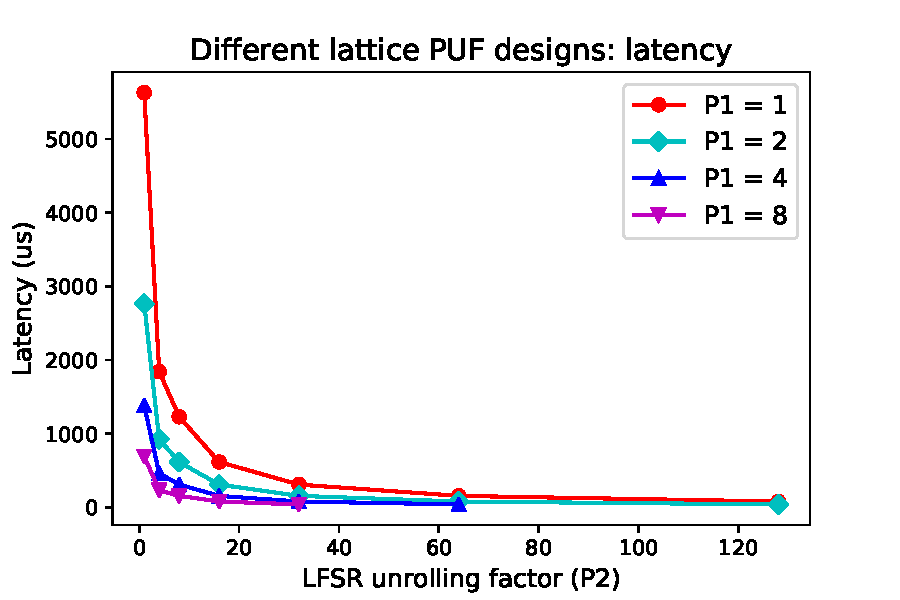
\includegraphics[width = 0.8\linewidth]{./figs/design_space_latency.pdf}
%\caption{Increasing $P_1$ and $P_2$ leads to steady reduction in latency.}
%\label{fig:design_space_latency}
%\end{figure}

%\begin{figure}[t!]
%\centering
%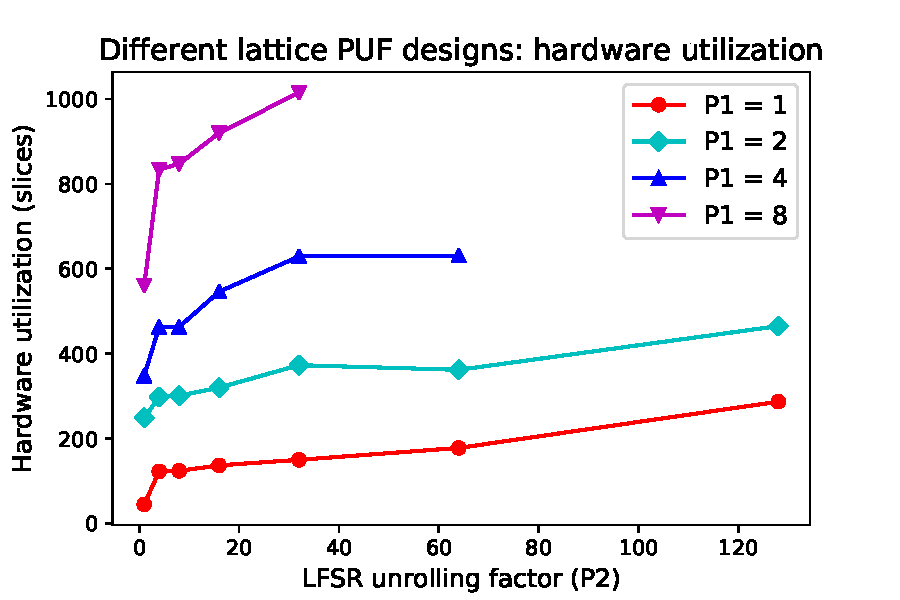
\includegraphics[width = 0.8\linewidth]{./figs/design_space_hw.pdf}
%\caption{Increasing $P_2$ is more hardware efficient than increasing $P_1$, but maximum $P_2$ is limited by the LFSR generator polynomial. The optimal strategy is to increase $P_2$ first to achieve latency goal. If $P_2$ reaches the limit and more aggressive latency reduction is required, increase $P_1$.}
%\label{fig:design_space_hw}
%\end{figure}

We finally compare the hardware utilization and latency of lattice PUF designs to several published strong PUF designs \cite{bhargava2014efficient, gassend2008controlled, jin2017fpga} who also have ML resistance in Table \ref{table:hardware_puf}. 
As mentioned in Section \ref{sec:intro}, there are two different categories of ML resistance among those listed PUFs. 
ML resistance of the AES-based PUF and the controlled PUF can be reduced to the security of the deployed primitives. 
In contrast, the theoretical ML resistance of the CFE-based strong PUF and our lattice PUF can be reduced to the hardness of fundamental math problems, like LPN and LWE.
The original proposal of the AES-based strong PUF \cite{bhargava2014efficient} is an ASIC implementation. 
Here, to estimate the AES implementation cost in FPGA, we adopt results in \cite{chu2012low}.
Note that the original proposal of \cite{bhargava2014efficient} does not use FE-based error correction: it uses dark bit masking to guarantee reliability. 
To estimate the cost of its error correction on an FPGA implementation, we use the RFE encoder design for a 128-bit key reconstruction with a $5\%$ raw BER and $10^{-6}$ failure rate, similar to the ECC design for the lattice PUF. The estimated number of raw POK bits are derived using these parameters.
Similarly, to calculate hash function hardware utilization in the controlled PUF \cite{gassend2008controlled}, the FPGA implementation results of SHA-3 in \cite{sha3_finalist} is used. 
No design details of the error correction and the POK are given in the proposal of controlled PUF \cite{gassend2008controlled}. We follow the same assumption as for the AES PUF for estimation.
\cite{jin2017fpga} reports the hardware utilization results of the computational FE (CFE) based strong PUF on FPGA in the LUT numbers.
By utilizing \cite{xilinx:ds190}, we convert the LUT numbers to the slice numbers. 
The CFE-based strong PUF does not use a conventional FE-based error correction so its ECC cost is 0.

Table \ref{table:hardware_puf} shows that the resource-efficient version of the lattice PUF achieves the smallest slice number among all strong PUF designs with ML resistance.
From the latency perspective, the AES-based PUF and the controlled PUF run faster than the CFE-based PUF and our lattice PUF. This is primarily due to the fundamental algorithmic difference of the LWE problem and the established cryptographic primitives. The LWE problem requires sequential MACs on the elements of long vectors and produces a single output bit per execution, while AES finishes within a relatively small number of rounds and has a much larger output size.
Compared to the CFE-based strong PUF whose ML resistance can also be reduced to the hardness of a fundamental math problem, the resource-efficient lattice PUF achieves a 205X area reduction, and the latency-optimized version achieves a 16X latency improvement together with a 19X area reduction.
%Recall that the ML resistance of the CFE-based strong PUF and our lattice PUF can be reduced to the hardness of fundamental math problems while strong PUFs based on AES or hash functions can 
%We achieve a great reduction in area compared to the CFE-based strong PUF \cite{herder2017trapdoor, jin2017fpga}, which gives theoretical ML-resistance similarly. 
%\textcolor{red}{In the performance-critical scenario, our design produces response bits faster than the CFE-based PUF \cite{herder2017trapdoor, jin2017fpga}, but slower than the AES PUF and the controlled PUF. This is primarily due to the fundamental algorithmic difference of the LWE problem and the established cryptographic primitives. The LWE problem requires sequential MACs on the elements of long vectors and produces a single output bit per execution, while AES finishes within a relatively small number of rounds and has a much larger output size.} %(We note that it is possible to further reduce latency of lattice PUF following our parallelization strategy, if implementing multipliers utilizing non-DSP slices. The cost will be significantly increased hardware utilization. We plan to investigate lattice PUF architectures which allows efficient further improvements in latency for future work.)} 
%We find that the implementation cost of the lattice PUF (without FE) is cheaper than that of AES on POK, controlled PUF, and CFE-based PUF.

%\textcolor{red}{Since the lattice PUF fundamentally builds upon a POK and an LWE decryption function, one natural question is if the POK can be replaced with a secret key programmed directly in non volatile memory. While this alternative primitive further reduces hardware cost, it compromises security that is otherwise provided by POK (PUF). The keys stored explicitly and permanently in memory can be easily exploited by physical access attacks \cite{semi_invasive_attacks}. In contrast, keys derived from PUFs only establish their values when evaluating the PUF. The nature of PUFs hide keys from physical access attacks since it explores intrinsic randomness of CMOS technology. Therefore, the lattice PUF primitive rather than the PUF-less alternative should be adopted for better security guarantees.}
%A lattice PUF is realized by two major components: a POK and an LWE decryption function. The POK is needed for silicon-intrinsic key generation, with all the well-known security benefits of PUF-based key generation. A simpler NVM-based key storage mechanism in place of the POK is an alternative approach that is cheaper but with reduced security against physical key-extraction attacks. In this case, the design described in the paper can be thought as a keyed LWE-based hash function with restricted inputs (which follow the ciphertext distribution).
%Note that there exists another such construction, namely, the LWE-based pseudorandom function \cite{brenner2014fpga}, which can even guarantee ML resistance without input restrictions.  In fact, its hardware implementation requires more logic slices.

\begin{figure}[t!]
\centering
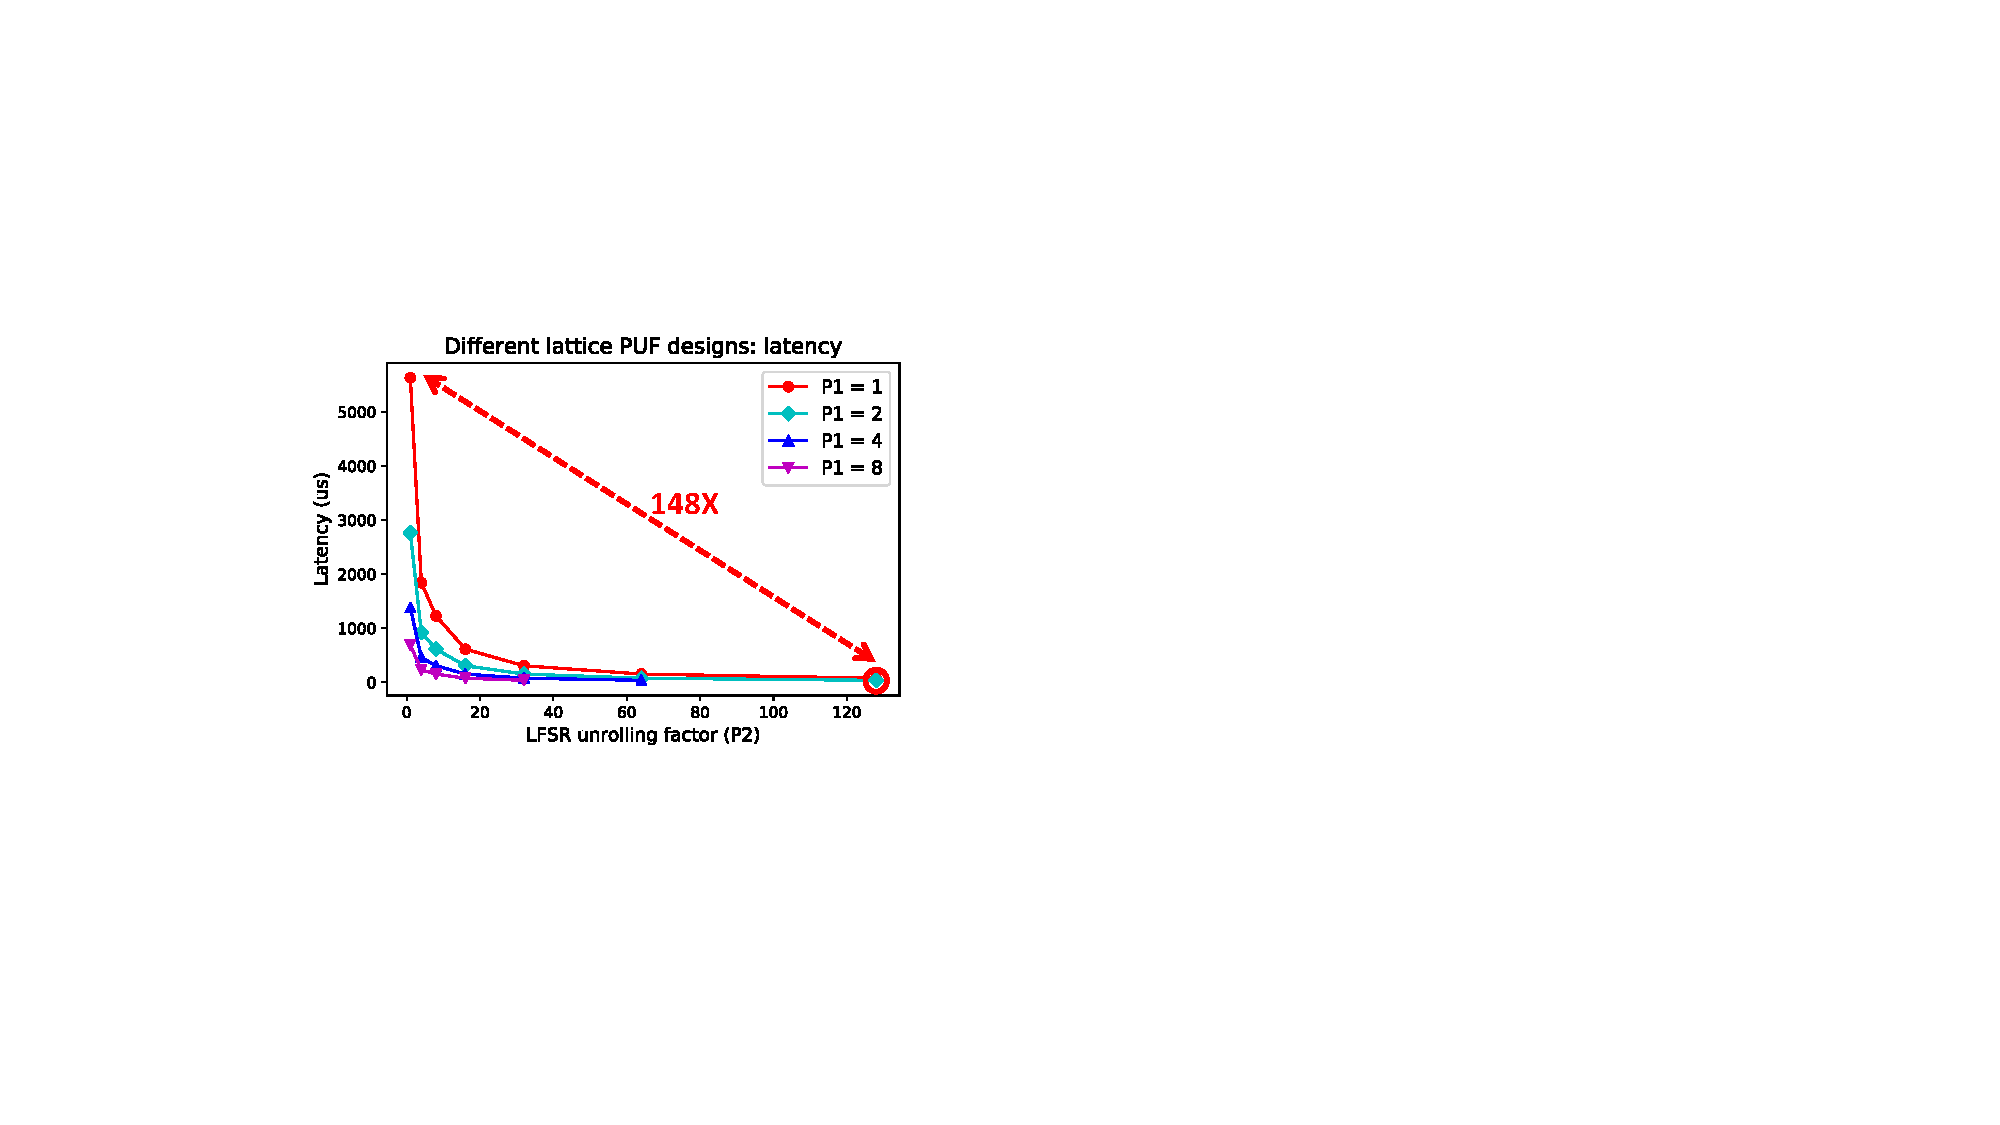
\includegraphics[width = 0.78\linewidth]{./figs/design_space_latency_annotated.pdf}
\caption{Increasing $P_1$ and $P_2$ leads to steady reduction in latency.}
\label{fig:design_space_latency}
\end{figure}

\begin{figure}[t!]
\centering
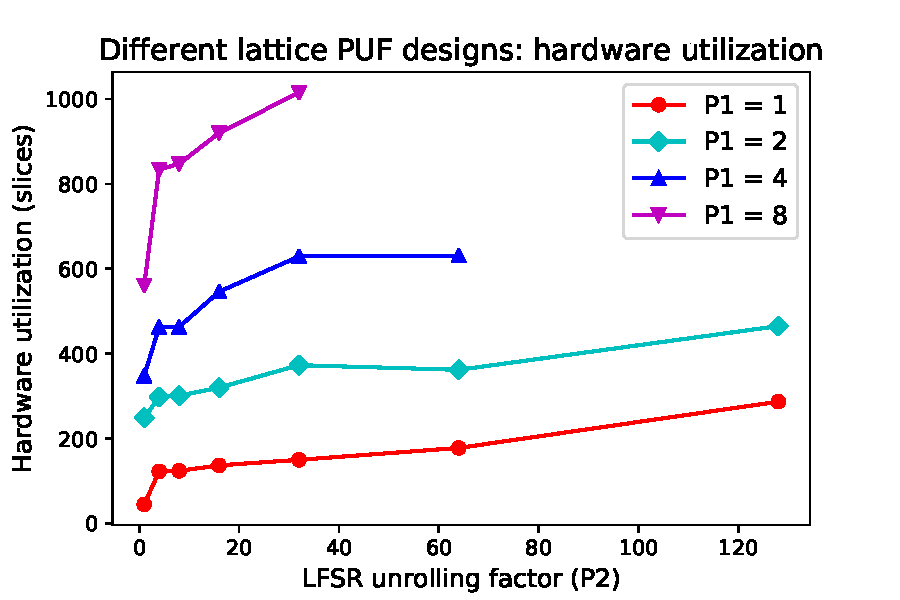
\includegraphics[width = 0.8\linewidth]{./figs/design_space_hw.pdf}
\caption{Increasing $P_2$ is more hardware efficient than increasing $P_1$, but maximum $P_2$ is limited by the LFSR generator polynomial. The optimal strategy is to increase $P_2$ first to achieve latency goal. If $P_2$ reaches the limit and more aggressive latency reduction is required, increase $P_1$.}
\label{fig:design_space_hw}
\end{figure}
\section{Conclusion}
\label{sec:conclusion}

We propose a novel strong PUF with theoretically proven security against ML attacks conducted by both classical and quantum computers. Its security is guaranteed by the cryptographic hardness to learn decryption functions of public key cryptosystems. Our PUF is constructed from the LWE decryption function block. A series of designs are implemented on a Xilinx Spartan-6 FPGA. A compact design uses a highly serialized LFSR and LWE decryption function, while a latency-optimized design uses an unrolled LFSR and a parallel datapath. The lattice PUF designs have a CRP space of $2^{136}$, with $6,360$ POK bits and $128$-bit concrete ML resistance. Excellent statistical characteristics are demonstrated.   
\section*{Acknowledgments}
We thank Dr.~Aydin Aysu for his insightful advice on idea presentation, assistance with FPGA implementation of repetition code, and comments that greatly improved the manuscript.

\bibliographystyle{abbrv}
\bibliography{refs/refs.bib}

\begin{IEEEbiography}[{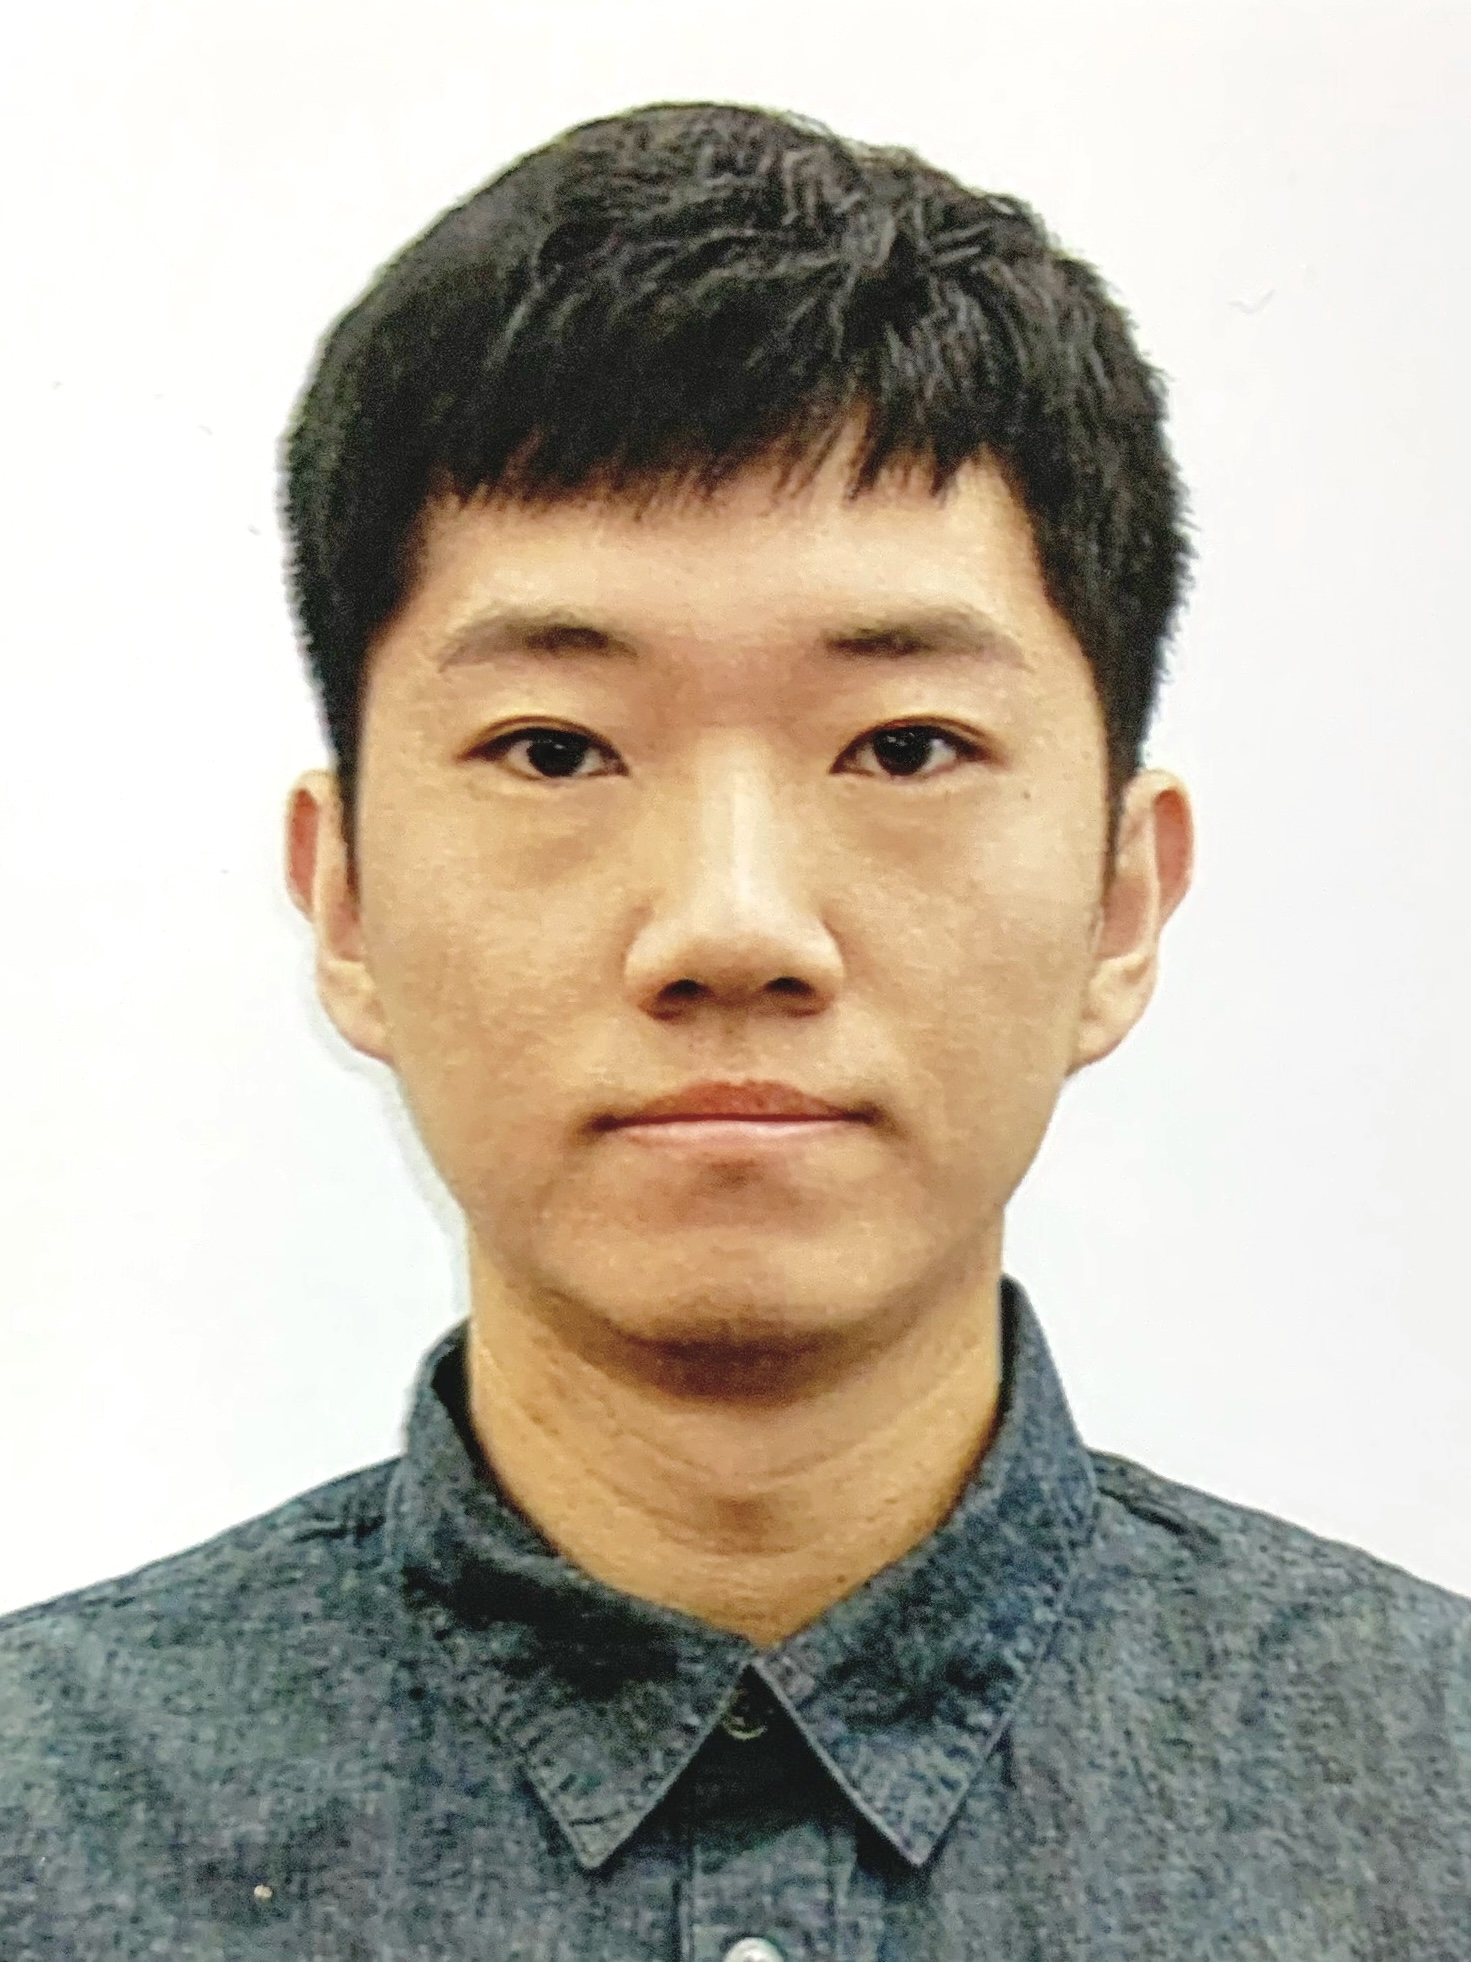
\includegraphics[width=1in,height=1.25in,clip,keepaspectratio]{./profiles/profile_xiaodan.jpg}}]%
{Xiaodan Xi}
received his M.S. and Ph.D. degree in Electrical and Computer Engineering from the University of Texas at Austin, Austin, TX, USA in 2016 and 2019. He received his B.S. degree in Electrical Engineering from Zhejiang University, Hangzhou, China in 2014. He is currently a software engineer at DoorDash, Austin, TX, USA. His research interests include security primitives such as physical unclonable function, side-channel analysis, and machine learning based attacks to security systems.
\end{IEEEbiography}

\begin{IEEEbiography}[{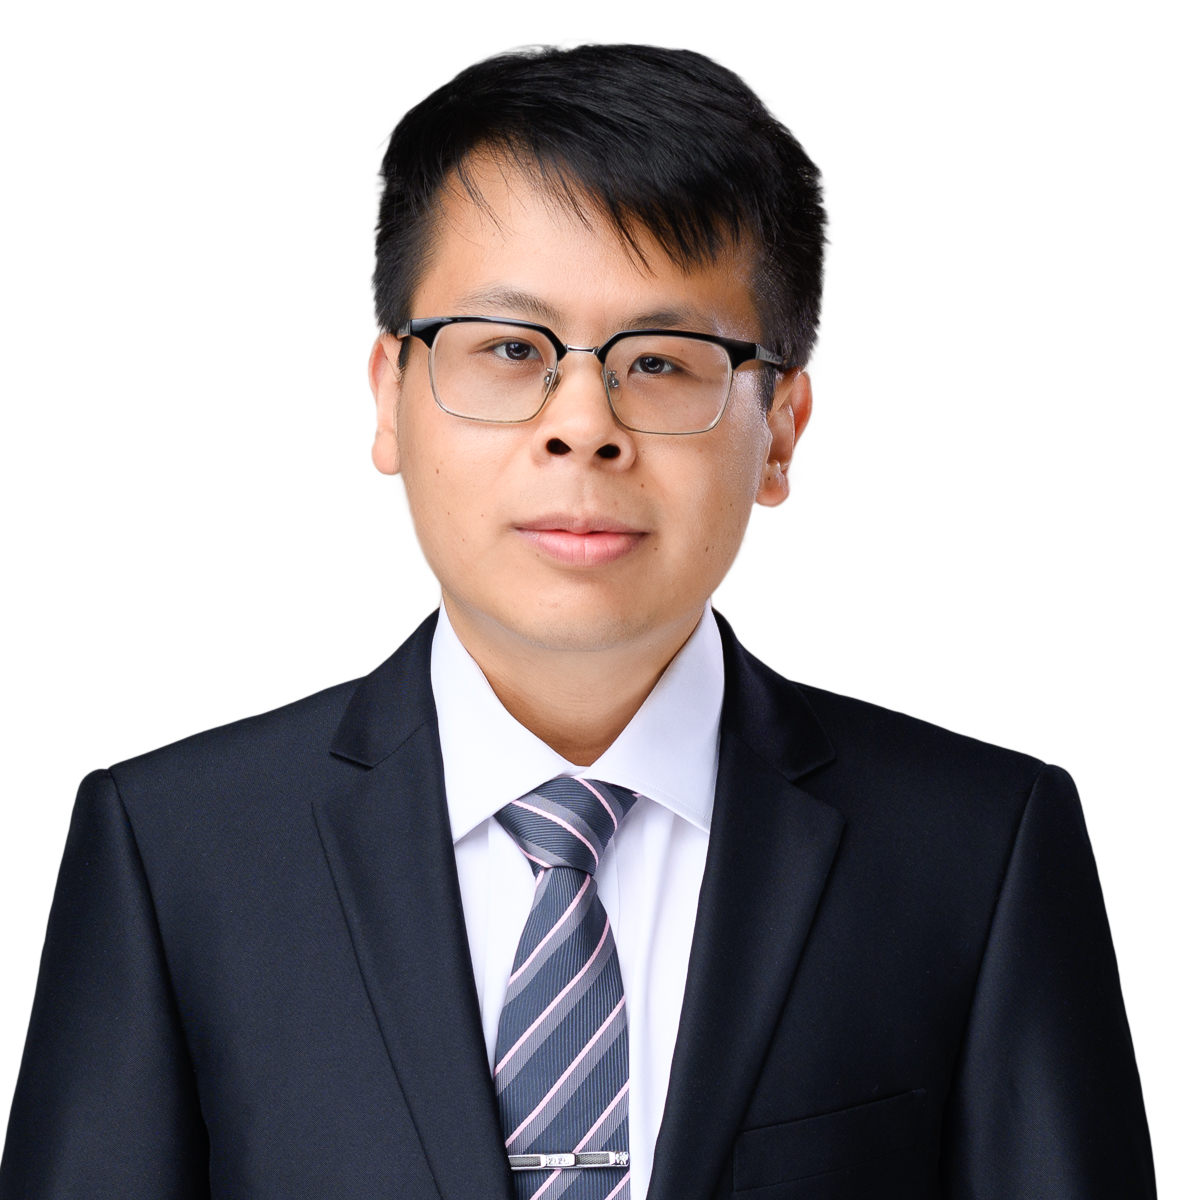
\includegraphics[width=1in,height=1.25in,clip,keepaspectratio]{./profiles/Ge Li.jpg}}]%
{Ge Li}
received his M.S. and Ph.D. degree in Electrical and Computer Engineering from the University of Texas at Austin, Austin, TX, USA in 2021 and 2022. He received his B.S. degree in Electronics Engineering and Computer Science from Peking University, Beijing, China, in 2017. His research interests include side channel analysis, side channel resilient VLSI design, machine learning based malware detection, physical unclonable functions and trustworthy AI.
\end{IEEEbiography}

\begin{IEEEbiography}[{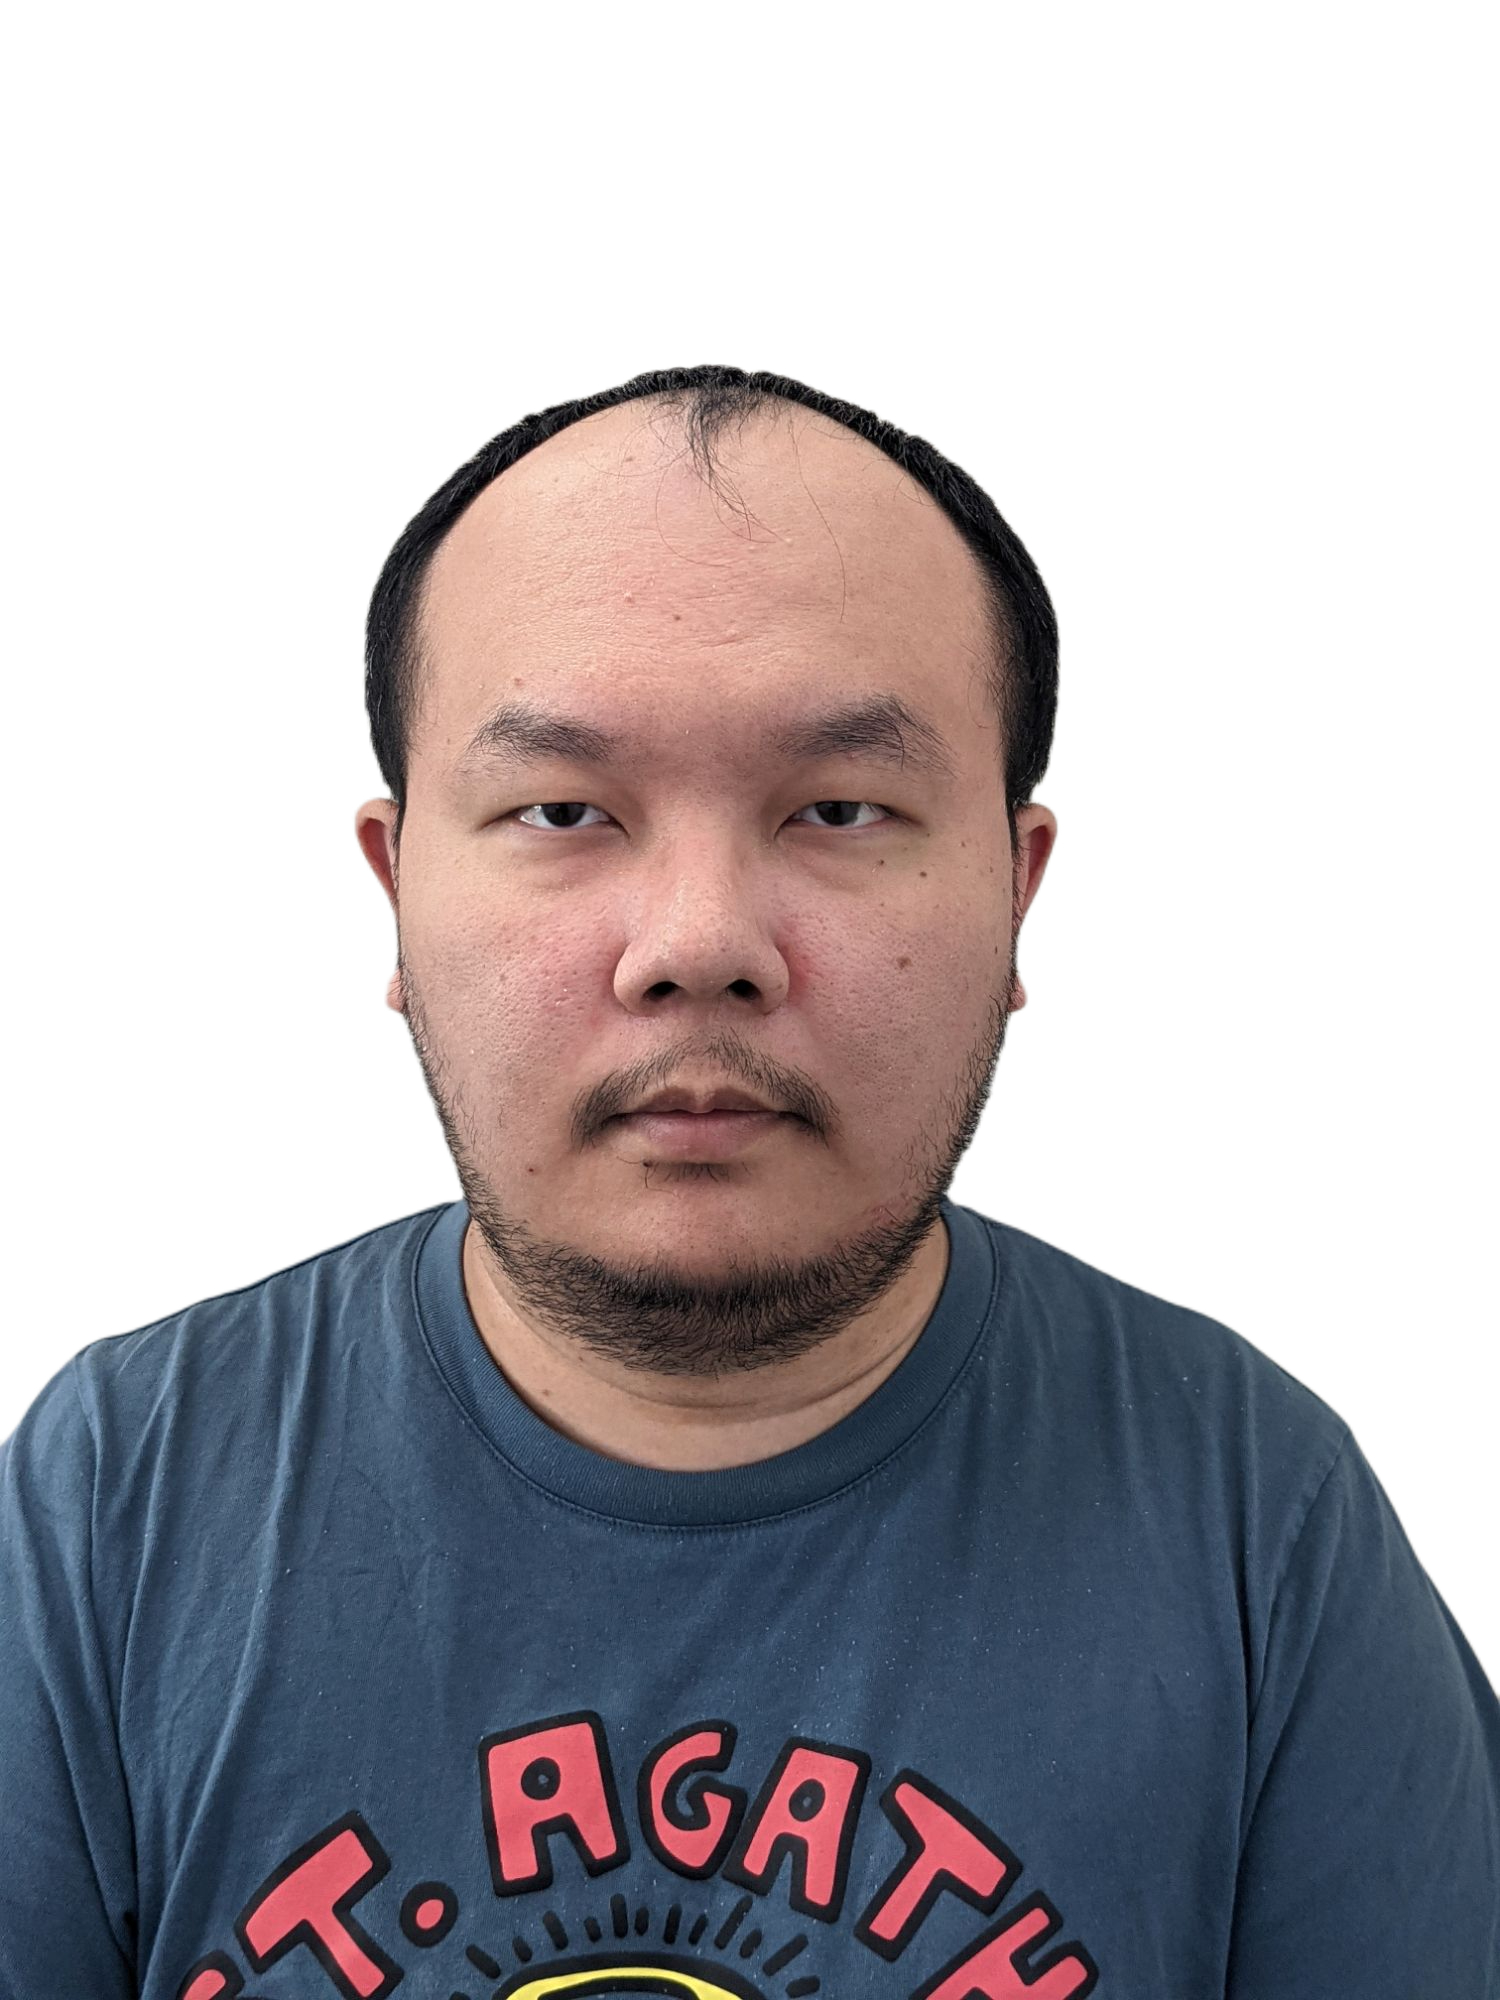
\includegraphics[width=1in,height=1.25in,clip,keepaspectratio]{./profiles/profile_yw.jpg}}]%
{Ye Wang}
received his M.S. and Ph.D. degree in Electrical and Computer Engineering from the University of Texas at Austin, Austin, TX, USA in 2015 and 2018, respectively. 
He received his B.S. degree in Electrical Engineering from Zhejiang University, China in 2012.
He is currently a software engineer at Youtube, Google. 
His research interests include recommendation system, hardware security, and numerical linear algebra.
\end{IEEEbiography}

\begin{IEEEbiography}[{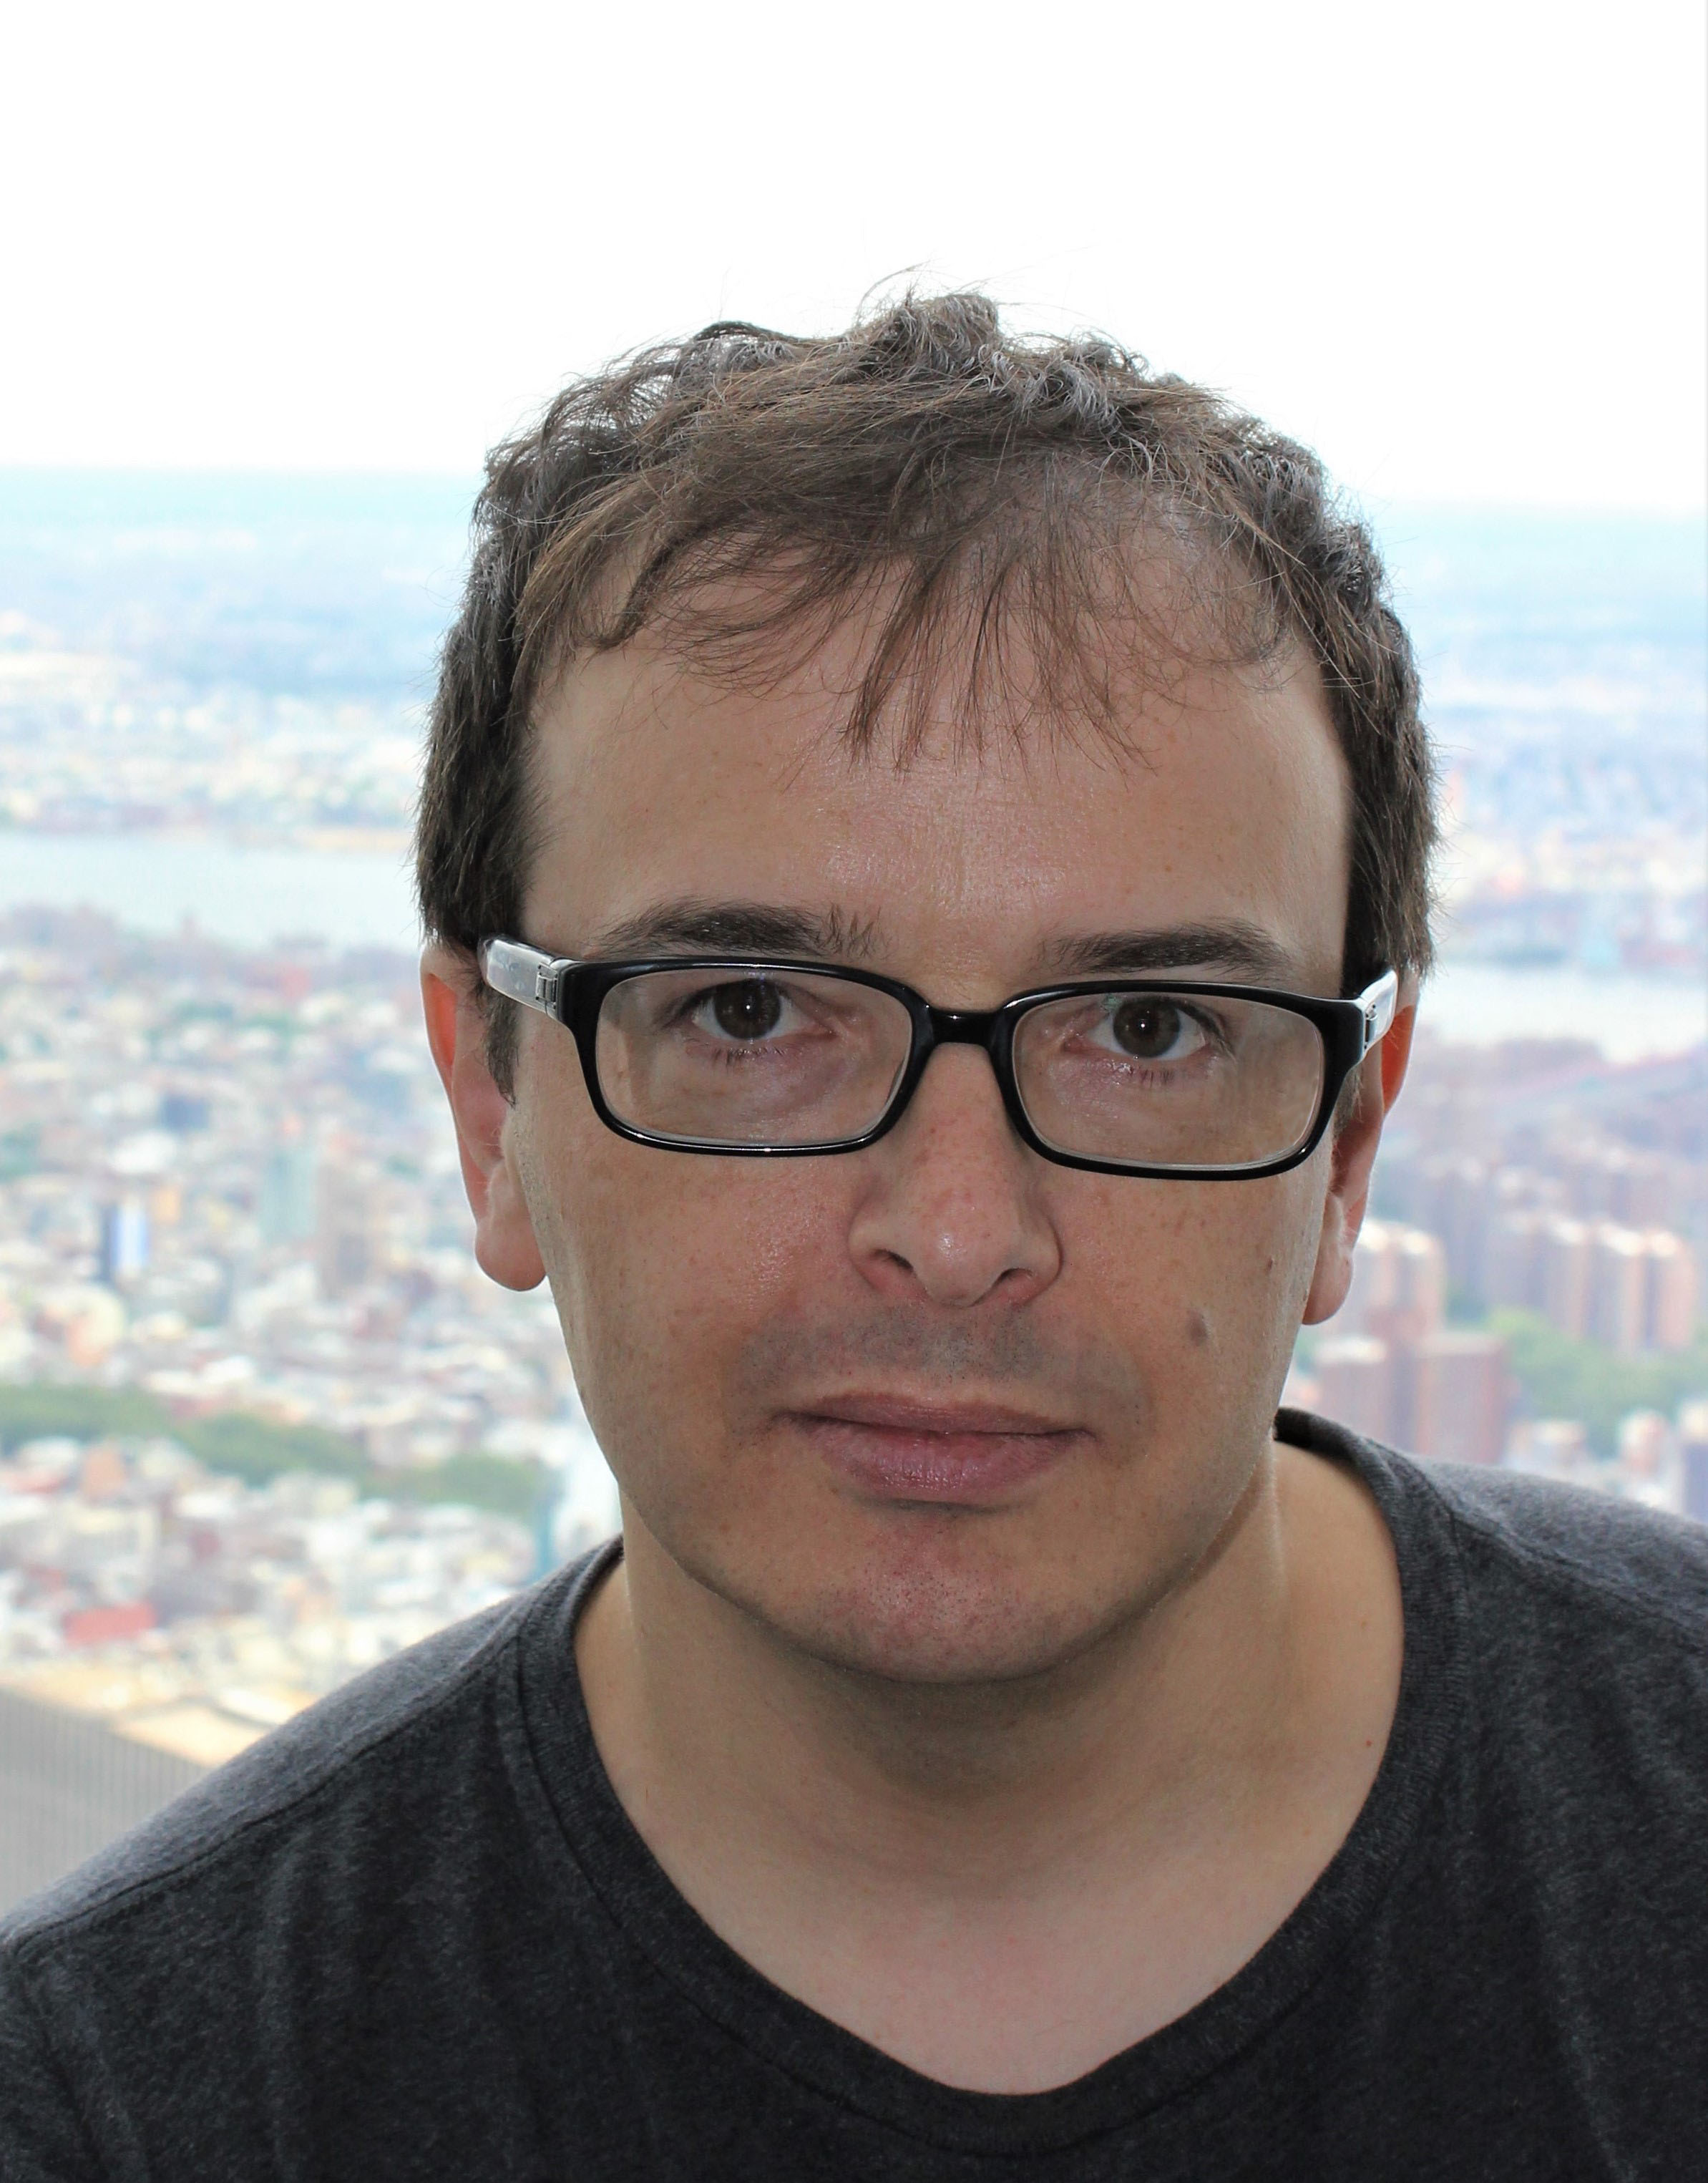
\includegraphics[width=1in,height=1.25in,clip,keepaspectratio]{./profiles/Orshansky.JPG}}]%
{Michael Orshansky} is a Professor of Electrical and Computer Engineering at the University of Texas at Austin and holds the John E. Kasch Endowed Faculty Fellowship in Engineering. He has published over a hundred technical articles and holds several U.S. patents. He is the author of the book “Design for Manufacturability and Statistical Design.” He has served as an Associate Editor for the IEEE Transactions on Computer-Aided Design of Integrated Circuits and Systems and IEEE Transactions on VLSI. His research interests are in hardware security, design for manufacturability, approximate computing, and HW accelerators of machine learning applications. He is the recipient of a number of awards for his research contributions and professional services. He is a Fellow of IEEE.
\end{IEEEbiography}


\end{document}
